%------------------------------------------------------------
% Pakete
%------------------------------------------------------------
\documentclass[12pt, parskip=half]{scrartcl}% Schriftgröße 12pt, Abstand zwischen Absätzen
\usepackage[utf8x]{inputenc}			%Wird für die direkte Eingabe von Umlauten gebraucht.
\usepackage[ngerman]{babel}				%Eine Sammlung von verschieden Sprachen, und ermöglicht für diese Sprachen die automatische Worttrennung und die ändert die Bezeichnungen in die jeweilige Sprache.
\usepackage[T1]{fontenc}				%westeuropäische Schriftkodierung verwenden
\usepackage{lmodern}					%andere Schriftart
\usepackage[babel=once]{csquotes}%Befleh \enquote für Anführungszeichen
\usepackage{amsmath, amssymb, amstext}	%Mathematische Erweiterungen
\usepackage[breaklinks]{hyperref}
\usepackage{graphicx} 					%Das Standardpaket zum Einbinden von Bildern / Grafiken. Kann auch zum Einbinden von PDF Seiten genutzt werden. 
\usepackage{pdfpages}					%Das Paket zum einbinden von PDF Dateien in ein LaTeX Dokument, wobei bei der Beamer Class das Paket graphicx dafür verwendet werden sollte.
\usepackage{setspace} 					%Damit kann der Zeilenabstand einfach geänderter zum 1.5 facher oder 2 facher Zeilenabstand.
\usepackage{xcolor} 					%Ermöglicht das Nutzen von Farben zum Beispiel farbige Schrift.
\usepackage{tikz} 						%Ist zwar dem Namen nach kein Programm zum Zeichen tikz - "tikz ist kein Zeichenprogramm". Es lassen sich damit dennoch schöne 	Bilder machen. Im Zusammenspiel mit gnuplot lassen sich auch Funktionen plotten.
\usepackage[section]{placeins}			%placeins ist ein Paket, welches verhindert, dass Floats hinter dem Befehl \FloatBarrier erscheint.
										%Der Standard Befehl \section{} wird so verändert, dass er immer einen \FloatBarrier am Anfang mit sich trägt.
\usepackage{geometry}					%Ermöglicht die einfacherer Einstellung der Seitenränder
\usepackage{listings}					%zum einbinden von Quelltext
\usepackage{todonotes}
\usepackage{caption} 					%Zum Ändern der Beschriftung von Tabellen und Bildern.
\usepackage{ulem}
\usepackage{verbatim}					%Zum erstellen von mehrzeiligen Kommentaren
%------------------------------------------------------------
% Dokumenteneinstellung
%------------------------------------------------------------
\geometry{a4paper, top=25mm, left=20mm, right=20mm, bottom=30mm, headsep=10mm, footskip=12mm}
\onehalfspacing							%Zeilenabstand 1.5
%\par\bigskip 
%\parindent=0pt							%verhindert das Einrücken
\lstset
{
	language=C,
	basicstyle=\tiny,
	keywordstyle=\color{blue}\ttfamily,
	stringstyle=\color{red}\ttfamily,
	commentstyle=\color{green}\ttfamily,
	showstringspaces=false,
	morecomment=[l][\color{magenta}]{\#}
}

%------------------------------------------------------------
% Deckblatt und Inhaltsverzeichnis
%------------------------------------------------------------
\begin{document}
	
%\input{./Deckblatt/Deckblatt.tex}
\pagenumbering{gobble}
\begin{titlepage}
	\vspace*{2.5cm}
	\begin{center}
		
		{\LARGE Modellbasierter Entwurf} \\ [1cm]
		\rule{\textwidth}{1pt}\\ [0.5cm]
		\textbf{\Huge {Neuronale Netze}}
		\rule{\textwidth}{1pt}\\[2cm]
		
		\begin{figure}[h]
			\centering
			
\includegraphics[width=0.2\linewidth]{./Bilder/Deckblatt/Beuth-Logo_single}
			\label{fig:Beuth-Logo_single}
		\end{figure}
		
		
		\bigskip 
		{\large BEUTH HOCHSCHULE FÜR TECHNIK BERLIN} \\
		University of Applied Sciences \\ 
		Fachbereich VI \\
		Technische Informatik\\ [5cm]
		
		\vfill	
		\large
		\begin{tabular}{|c|c|} %Teilnehmer
			\hline
			\textbf{Teilnehmer} & \textbf{Matrikelnummer} \\ 
			\hline 
			Bryan Scheffner & 888777 \\ 
			%\hline 
			Toni Reichel & 897991 \\ 
			\hline 
		\end{tabular}
		\normalsize
	\end{center}
\end{titlepage}

\tableofcontents
\newpage
		
%------------------------------------------------------------
% ab hier beginnt das eigentliche Dokument
%------------------------------------------------------------
\newcommand{\faq}[2]{%
	{\scshape Frage:} \normalfont\sffamily\textsf{#1}\par
	\noindent{\scshape Antwort:} #2
}
\pagenumbering{arabic} 
\section{Einleitung}

\subsection{Motivation neuronaler Netze}
Heutzutage findet man in nahezu allen Bereichen des Lebens Programme vor, sei es in Zahnbürsten, Autos oder in Robotern am Fließband. Mithilfe von Programmen sollen also sich wiederholende Aufgaben vereinfacht oder automatisiert werden. Dafür werden die Programme mit prozedurale oder objektorientierte Methoden entwickelt. Bevor mit der Programmierung angefangen werden kann, muss zuerst ein Modell des Problems entworfen werden. Bei einfachen Anwendungen, wie zum Beispiel einer Zahnbürste ist es recht einfach. Möchte man allerdings ein Modell für eine Mustererkennung 

\subsection{Das menschliche Nervensystem}
Das menschliche Gehirn besteht aus etwa 86 Milliarden Nervenzellen, auch Neuronen genannt, die zum Zentralnervensystem miteinander verschaltet sind (im folgendem Nervensystem). Nervenzellen im Gehirn sind hochspezialisierte Zellen, die sich im Gegensatz zu einfacheren Zellen nicht teilbar sind. Das bedeutet, dass sich das Nervensystem nicht über Zellteilung regenerieren kann. Allerdings schafft es das Gehirn durch die Verknüpfung anderer Nervenzellen den Defekt teilweise oder komplett auszugleichen. Jede Nervenzelle kann mit bis zu 10.000 anderen Nervenzellen in Verbindung stehen. 

Jede Nervenzelle ist zwar im Grundaufbau gleich, kann aber unterschiedliche Formen und Größen haben. Das liegt unter anderem daran, dass sich Nervenzellen weiter spezialisieren. So können die einen Nervenzellen eher für motorische und die anderen eher für sensorische Aufgaben bestimmt sein. Dadurch erreichen Nervenzellen unterschiedliche Geschwindigkeiten, wie sie Informationen an andere Nervenzellen weitergeben. Der Informationsfluss ist dabei immer in die gleiche Richtung. In Abbildung \ref{AufbauNeuron} ist der Aufbau einer Nervenzelle dargestellt.

\begin{figure}[hbt]
	\centering
	\includegraphics[width=0.9\linewidth]{./Bilder/Aufbau_Gehirn_gehirnlernen-de}
	\caption{Aufbau Neuron}
	\label{AufbauNeuron}
\end{figure}

Der hier stark vereinfachte Aufbau einer Nervenzelle besteht aus dem Zellkörper, den Dendriten, dem Axon und den Synapsen. Der Zellkörper bildet die zentrale Einheit einer Nervenzelle und erhält seine Informationen über die Dendriten. Die Dendriten sind baumartig verzweigt und mit anderen Nervenzellen über Synapsen verbunden. Der Zellkörper bildet eine Summation über die Signale der vielen verschieden Dendriten. Dabei kann jedes Dendrit eine erregende oder hemmende Wirkung auf den Zellkörper haben. Bei ausreichender Stärke leitet der Zellkörper das Signal weiter. Wenn eine Erregungsweiterleitung stattfindet, wird das Signal über das Axon und Synapsen an die nächste Nervenzelle weitergeleitet. Ein Axon hat einen Durchmesser von 0,002 - 0,01 Millimetern und kann bis zu einem Meter lang sein. Umso dicker ein Axon ist, desto schneller findet auch die Weiterleitung statt. Jede Nervenzelle kann nur über ihre Synapsen mit anderen Nervenzellen kommunizieren. Dafür hat jede Nervenzelle bis zu 10.000, in manchen Extremfälle sogar mehr als 100.000 Synapsen. Synapsen kommunizieren untereinander mit chemischen oder elektrischen Signalen. Wobei elektrische in chemische und chemische in elektrische Signale umgewandelt werden. In der Regel kommunizieren Synapsen über chemische Signale. Der Grund dafür ist, dass Synapsen meisten keinen direkten Kontakt zueinander haben, sondern ein kleiner Abstand von 20 bis 50 Nanometern bleibt. Bei elektrischen Synapsen ist der Abstand so nah, dass über eine kleine Brücke (gap junction) kommuniziert wird. Dabei kann das Signal schneller weitergeleitet werden.

Das Nervensystem ist ein großes Netz aus sehr vielen Nervenzellen, die unterschiedlich stark miteinander verbunden sind und unterschiedlich schnell Signale weiterleiten. Wenn eine Nervenzelle ein Signal auslöst, weil eine gewisse Schwelle überschritten wurde spricht man auch davon, dass das Aktionspotenzial erreicht wurde. Das Aktionspotenzial kann nur erreicht werden, wenn vorher genügend vorgeschaltete Nervenzellen ein Signal gesendet haben. Der Anfang einer Verkettung von Nervenzellen kann zum Beispiel über sehen, schmecken, spüren oder ähnliches stattfinden. Wird ein Aktionspotenzial in den dafür verantwortlichen Nervenzellen erreicht, werden sie wieder Signale an andere Nervenzellen senden. Am Ende kann das Signal bei Nervenzellen ankommen, die für eine Bewegung verantwortlich sind, wie zum Beispiel eine Gehbewegung. Das ist ein sehr stark vereinfachtes Beispiel und soll nur dazu dienen die Mechanismen eines Nervensystems zu verstehen.

Dieser Text Falls im Text in diesem Abschnitt nicht anders angegeben sind über die Quellen \cite{dasgehirn.info} und \cite{gehirnlernen.de} zu finden.
\newpage
\section{Aufbau des neuronalen Netzes}

In diesem Abschnitt wird erklärt, wie unser neuronales Netz aufgebaut ist. Vor allem die Abbildung \ref{AnordungMerkuPix} ist für das bessere Verständnis der Matlab-Skripte wichtig. In den Matlab-Skripten muss immer die Pixelanzahl und die Merkmalanzahl angegeben werden. Dabei handelt es sich immer um einen symmetrischen Aufbau. Ist die Merkmalanzahl gleich 5, dann gibt es 25 Merkmale (5 in x-Richtung und 5 in y-Richtung). Das gleiche gilt für die Pixelanzahl. Bei einer Pixelanzahl von 8 werden für jedes Merkmale 8 mal 8 Pixel angenommen. Bei einer Merkmalanzahl von 5 und einer Pixelanzahl von 8 wird also eine Pixelmatrix von 40 mal 40 Pixel erzeugt.

\begin{figure}[hbt]
	\centering
	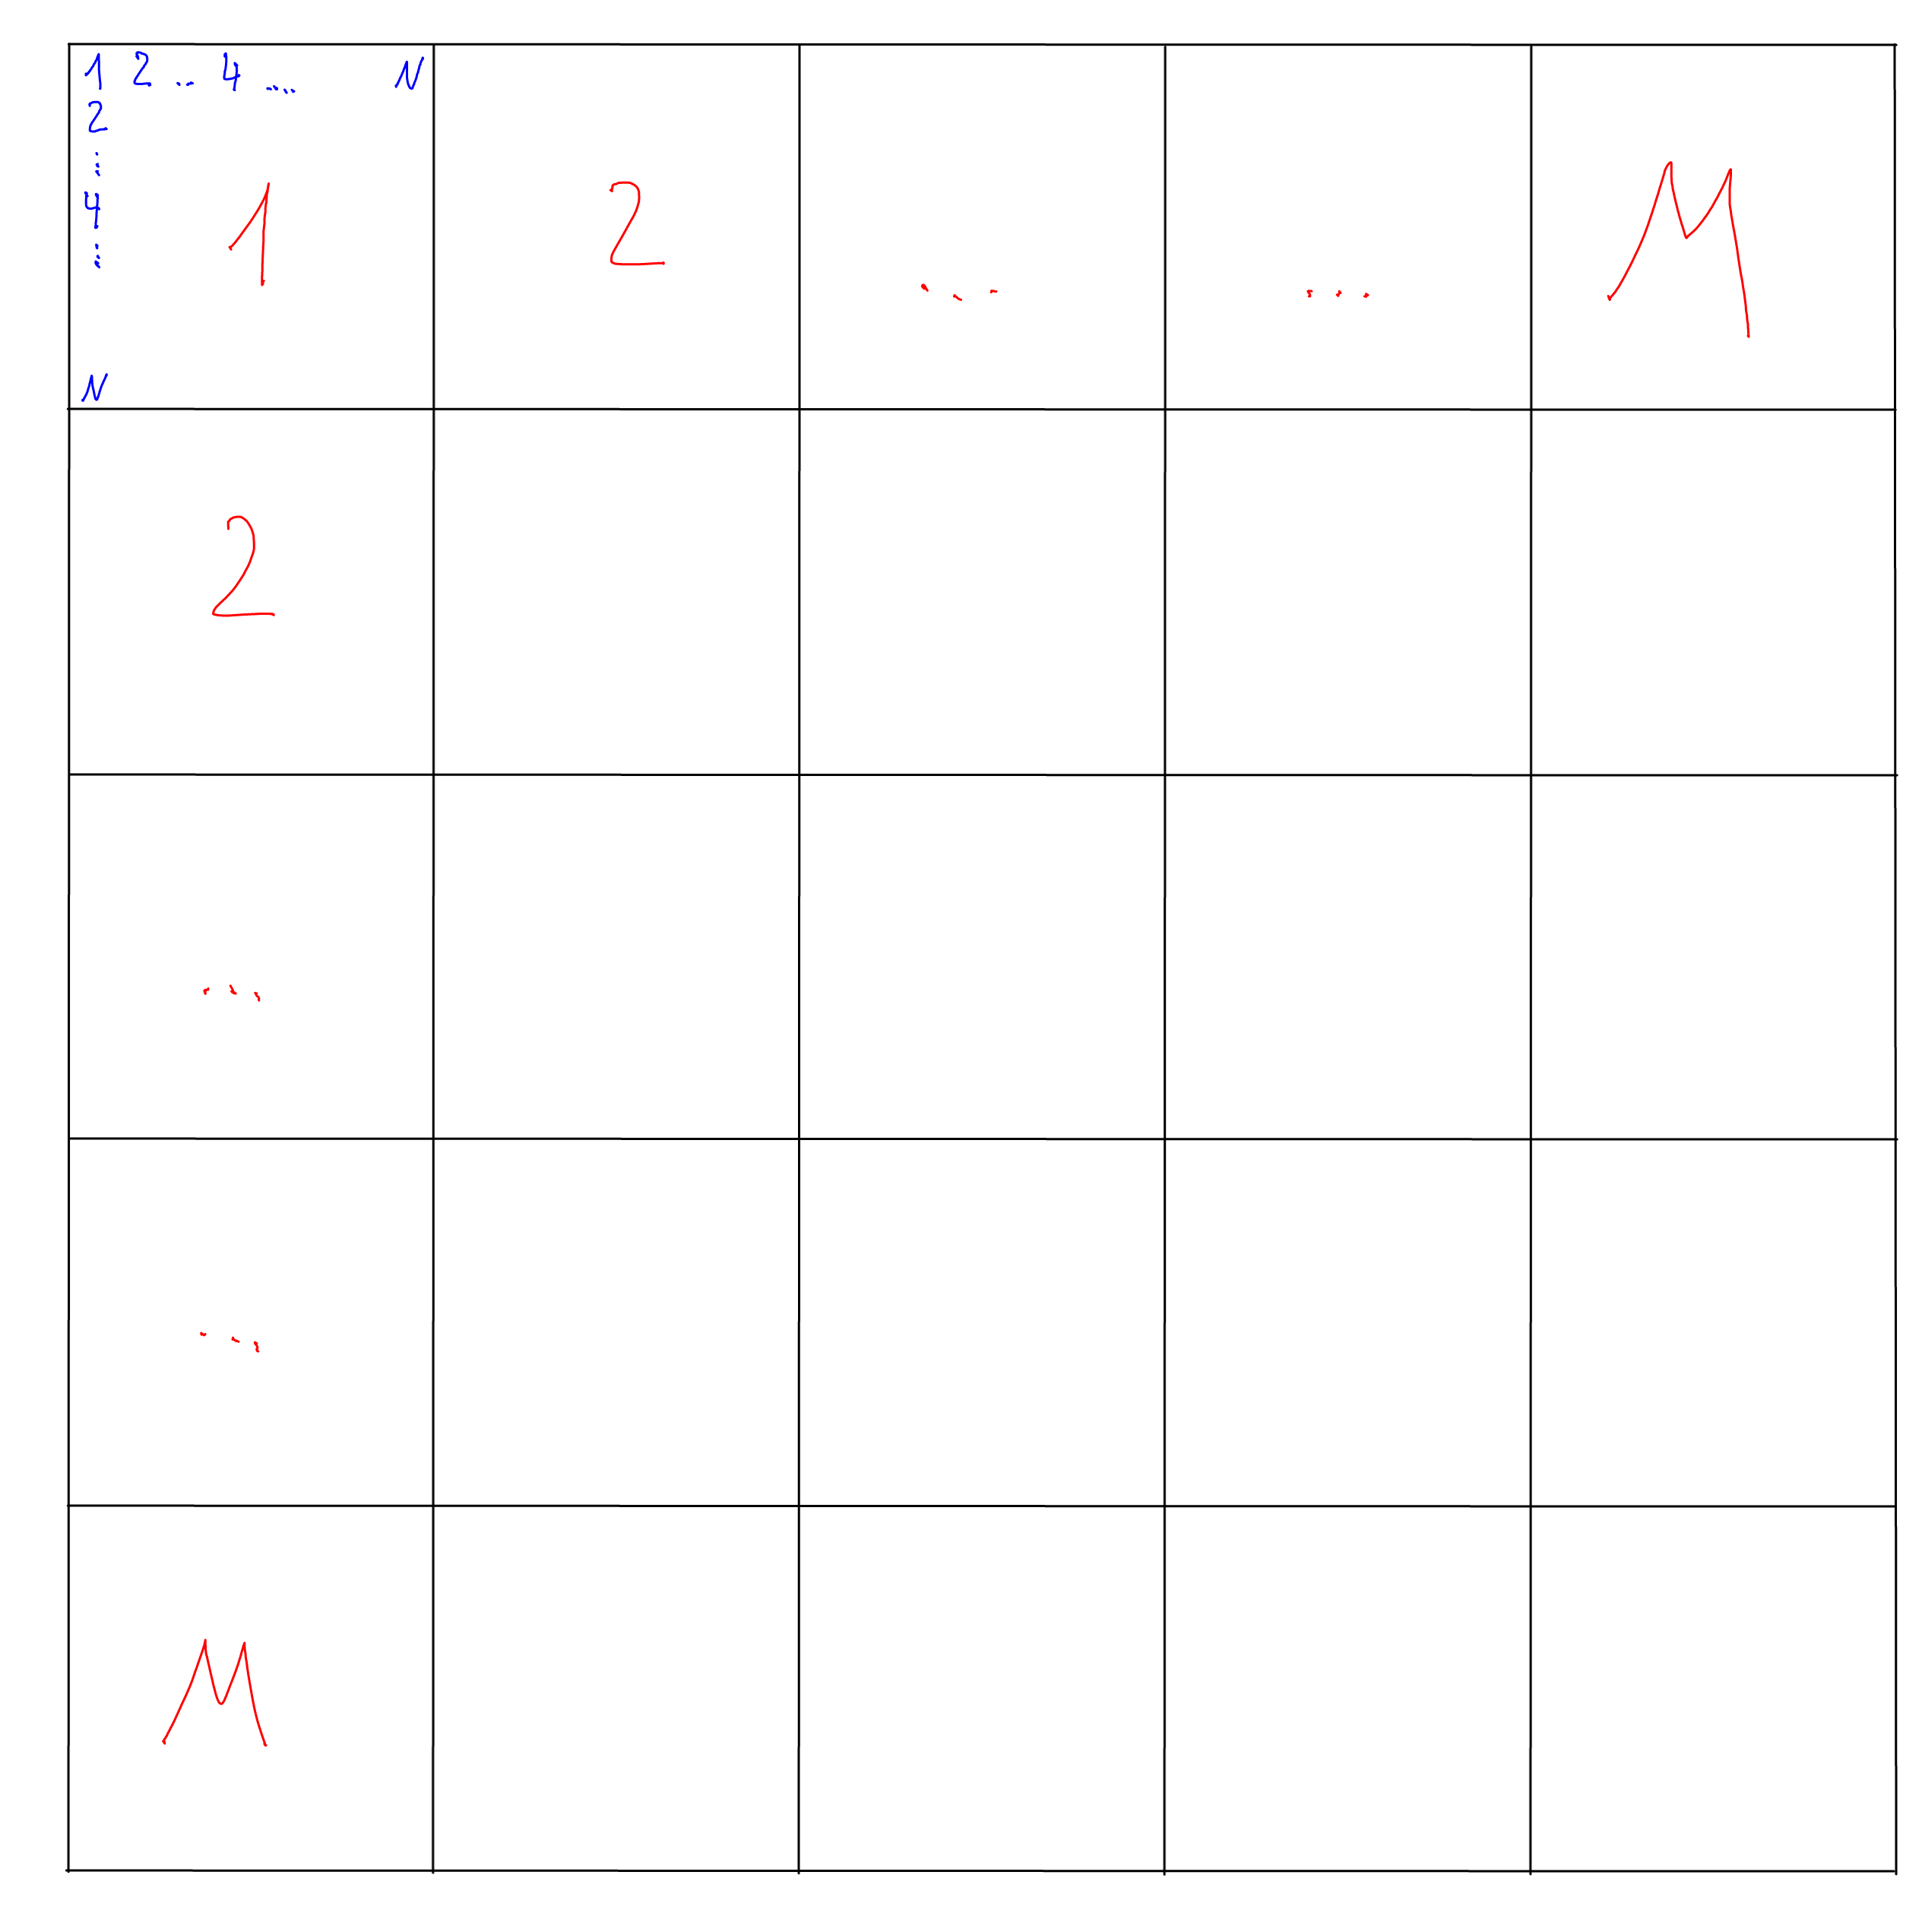
\includegraphics[width=0.5\linewidth]{./Bilder/Auswertung/Aufbau/page4}
	\caption{Anordnung der Merkmale und Pixel}
	\label{AnordungMerkuPix}
\end{figure}

In Abbildung \ref{Neuron1Ebene} ist ein Neuronenbeispiel abgebildet. Dieses Neuron der 1. Ebene fasst ein komplettes Merkmal mit all seinen Pixel zusammen. Dieses Neuron hat also in unserem Beispiel 64 Eingänge und es gibt 25 solcher Neuronen.

\begin{figure}[hbt]
	\centering
	
\includegraphics[width=0.6\linewidth]{./Bilder/Auswertung/Aufbau/page5}
	\caption{Neuron der 1. Ebene}
	\label{Neuron1Ebene}
\end{figure}

Mit einer einzigen Ebene von Neuronen kann sehr viel erreicht werden. Allerdings ist für die Gesamtauswertung eine zweite Ebene von Vorteil, um zum Beispiel bei starkem Rauschen Fehler besser zu detektieren. Bevor wir uns die zweite Ebene der Neuronen angucken, werfen wir einen Blick auf die Abbildung \ref{Erl2Ebene}. Hier sind drei Arten von Merkmalen zu erkennen. Die fünf schwarzen Merkmale detektieren einen horizontalen Balken, die blauen Merkmale einen vertikalen Balken und die roten Merkmale können hohes Rauschen beziehungsweise auch Fehler detektieren. Die roten Merkmale erlauben es, eine bessere Konfiguration des neuronalen Netzes zu finden.

\begin{figure}[hbt]
	\centering
	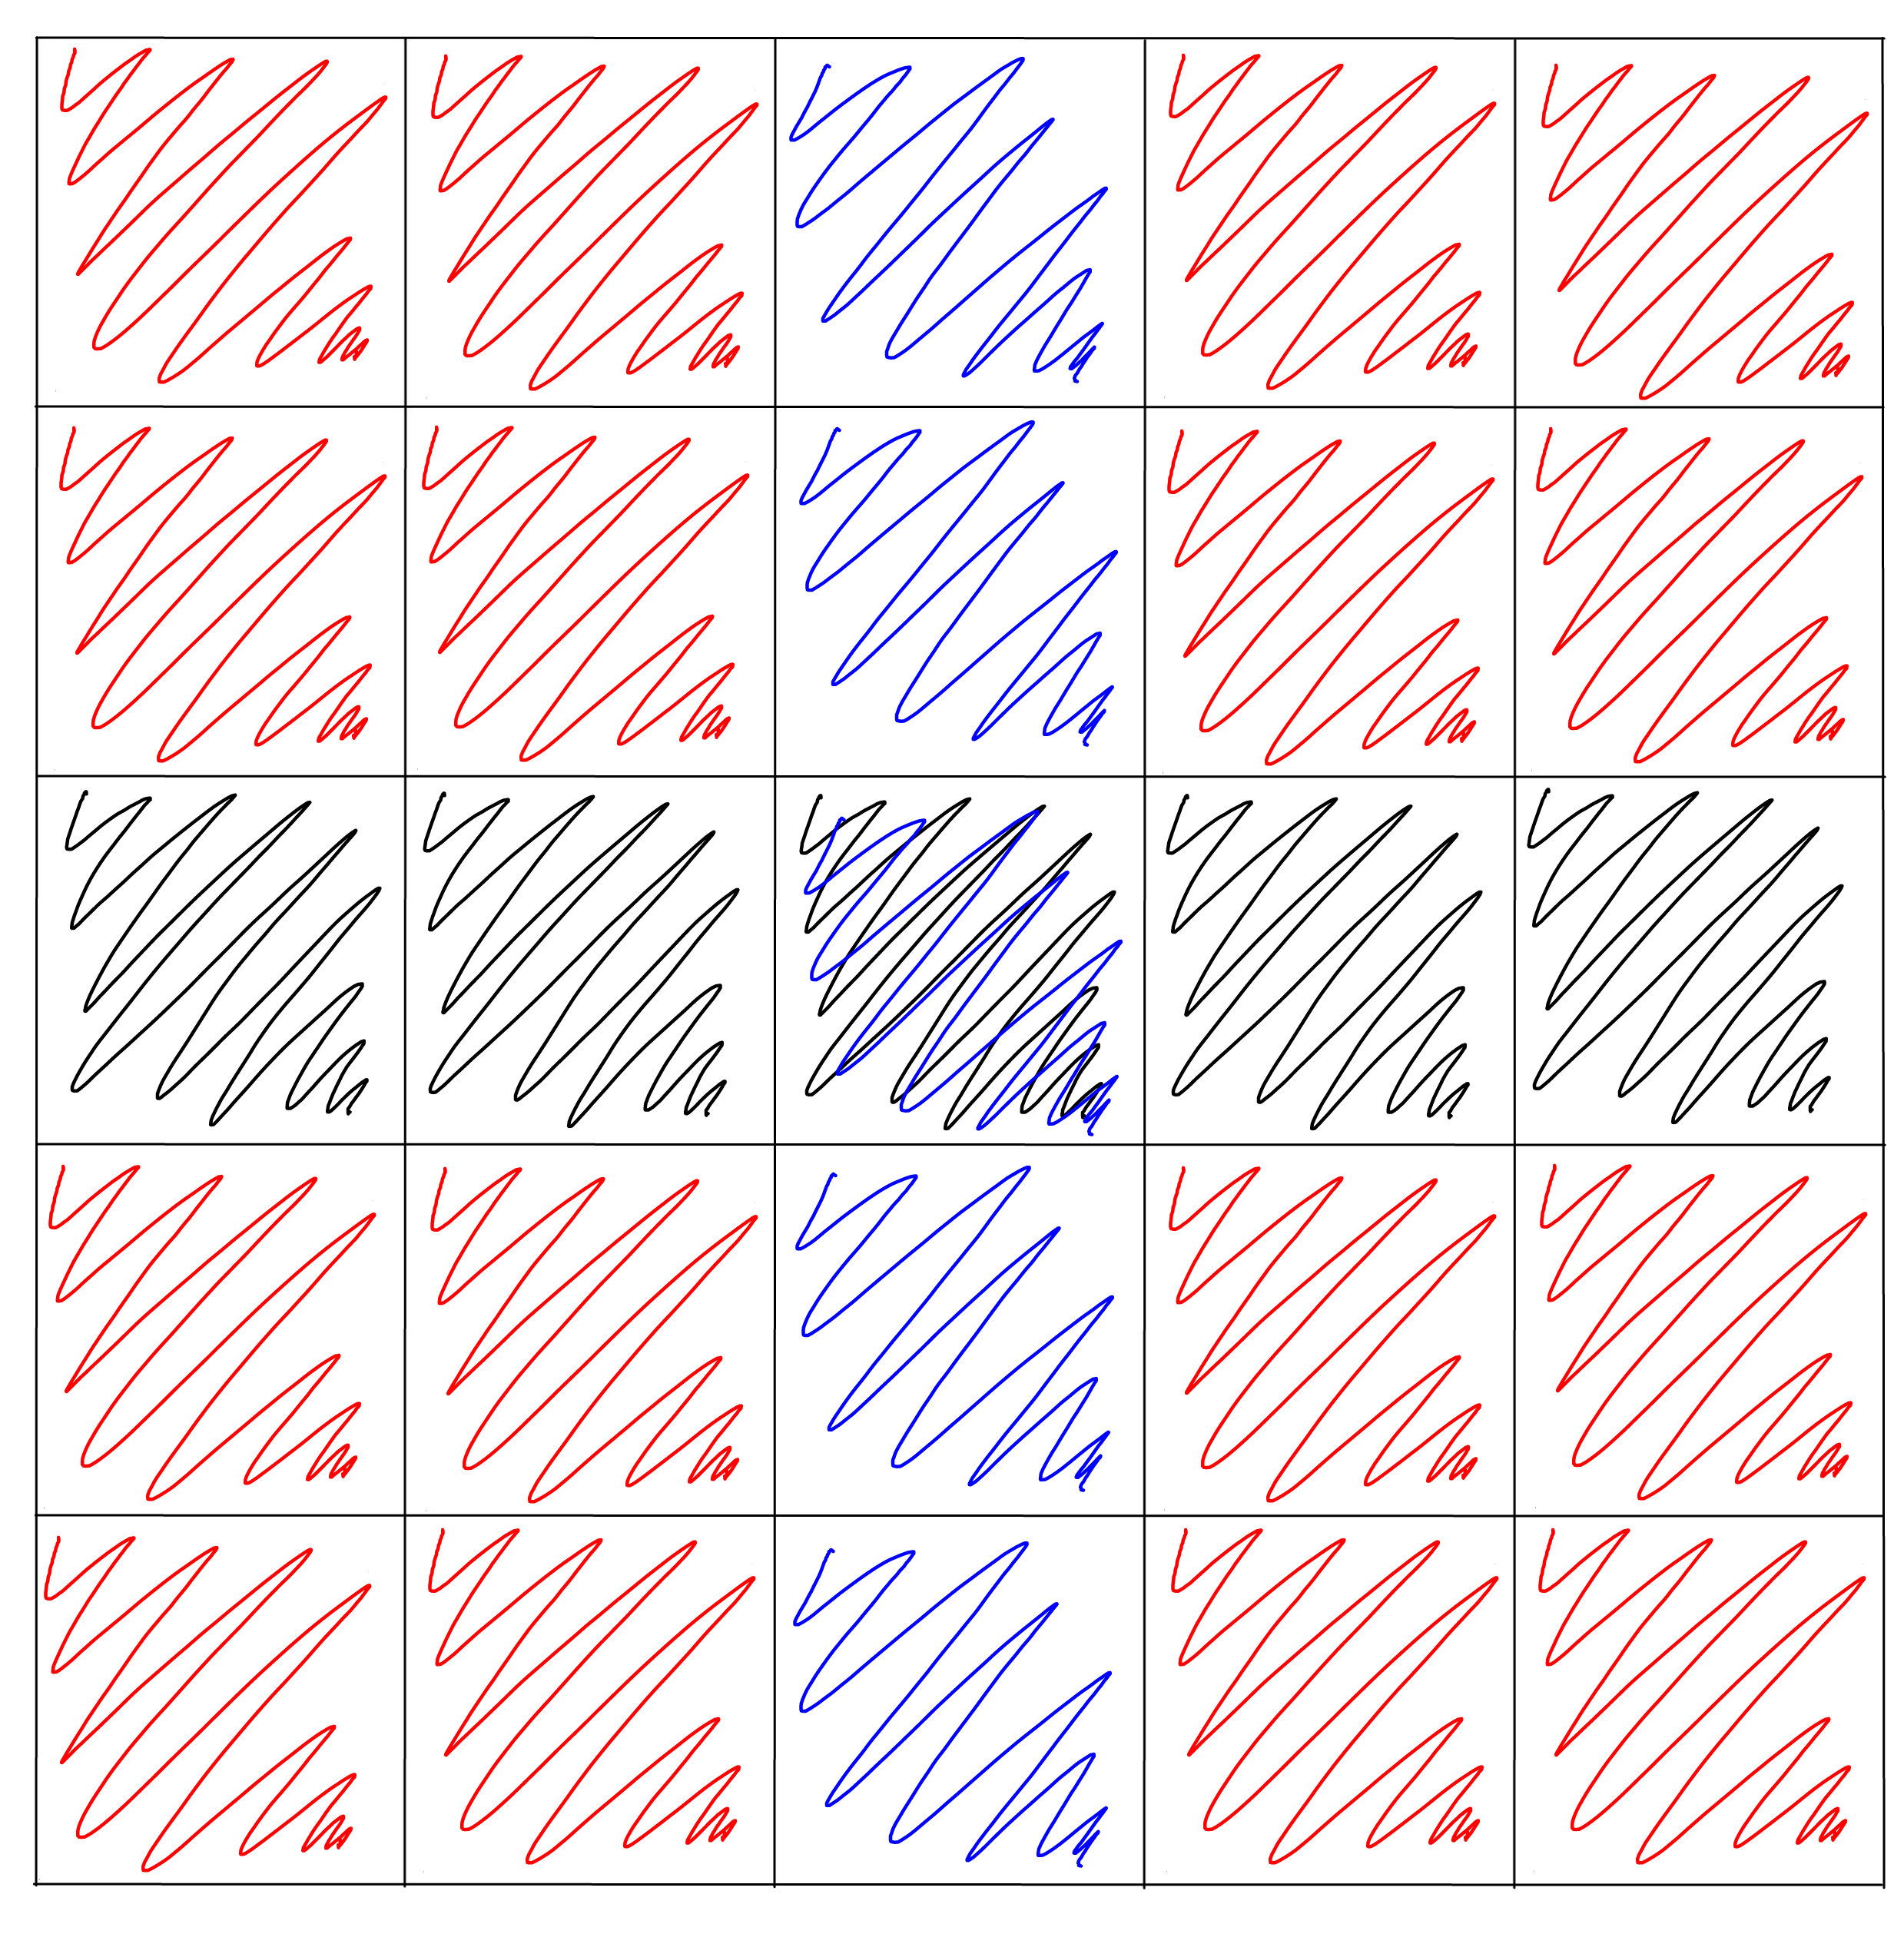
\includegraphics[width=0.6\linewidth]{./Bilder/Auswertung/Aufbau/page6}
	\caption{Erläuterung der Anordnung für die 2. Ebene}
	\label{Erl2Ebene}
\end{figure}

In Abbildung \ref{Neurin2Ebene} ist die komplette zweite Ebene des Neuronalen Netzes dargestellt. Alle drei Merkmale-Typen werden jeweils auf ein Neuron gegeben. In diesem Fall sind alle Gewichte auf eins gesetzt. Es muss nur der Bias eingestellt und somit eine Schwelle zur Detektion festgelegt werden. 

\begin{figure}[hbt]
	\centering
	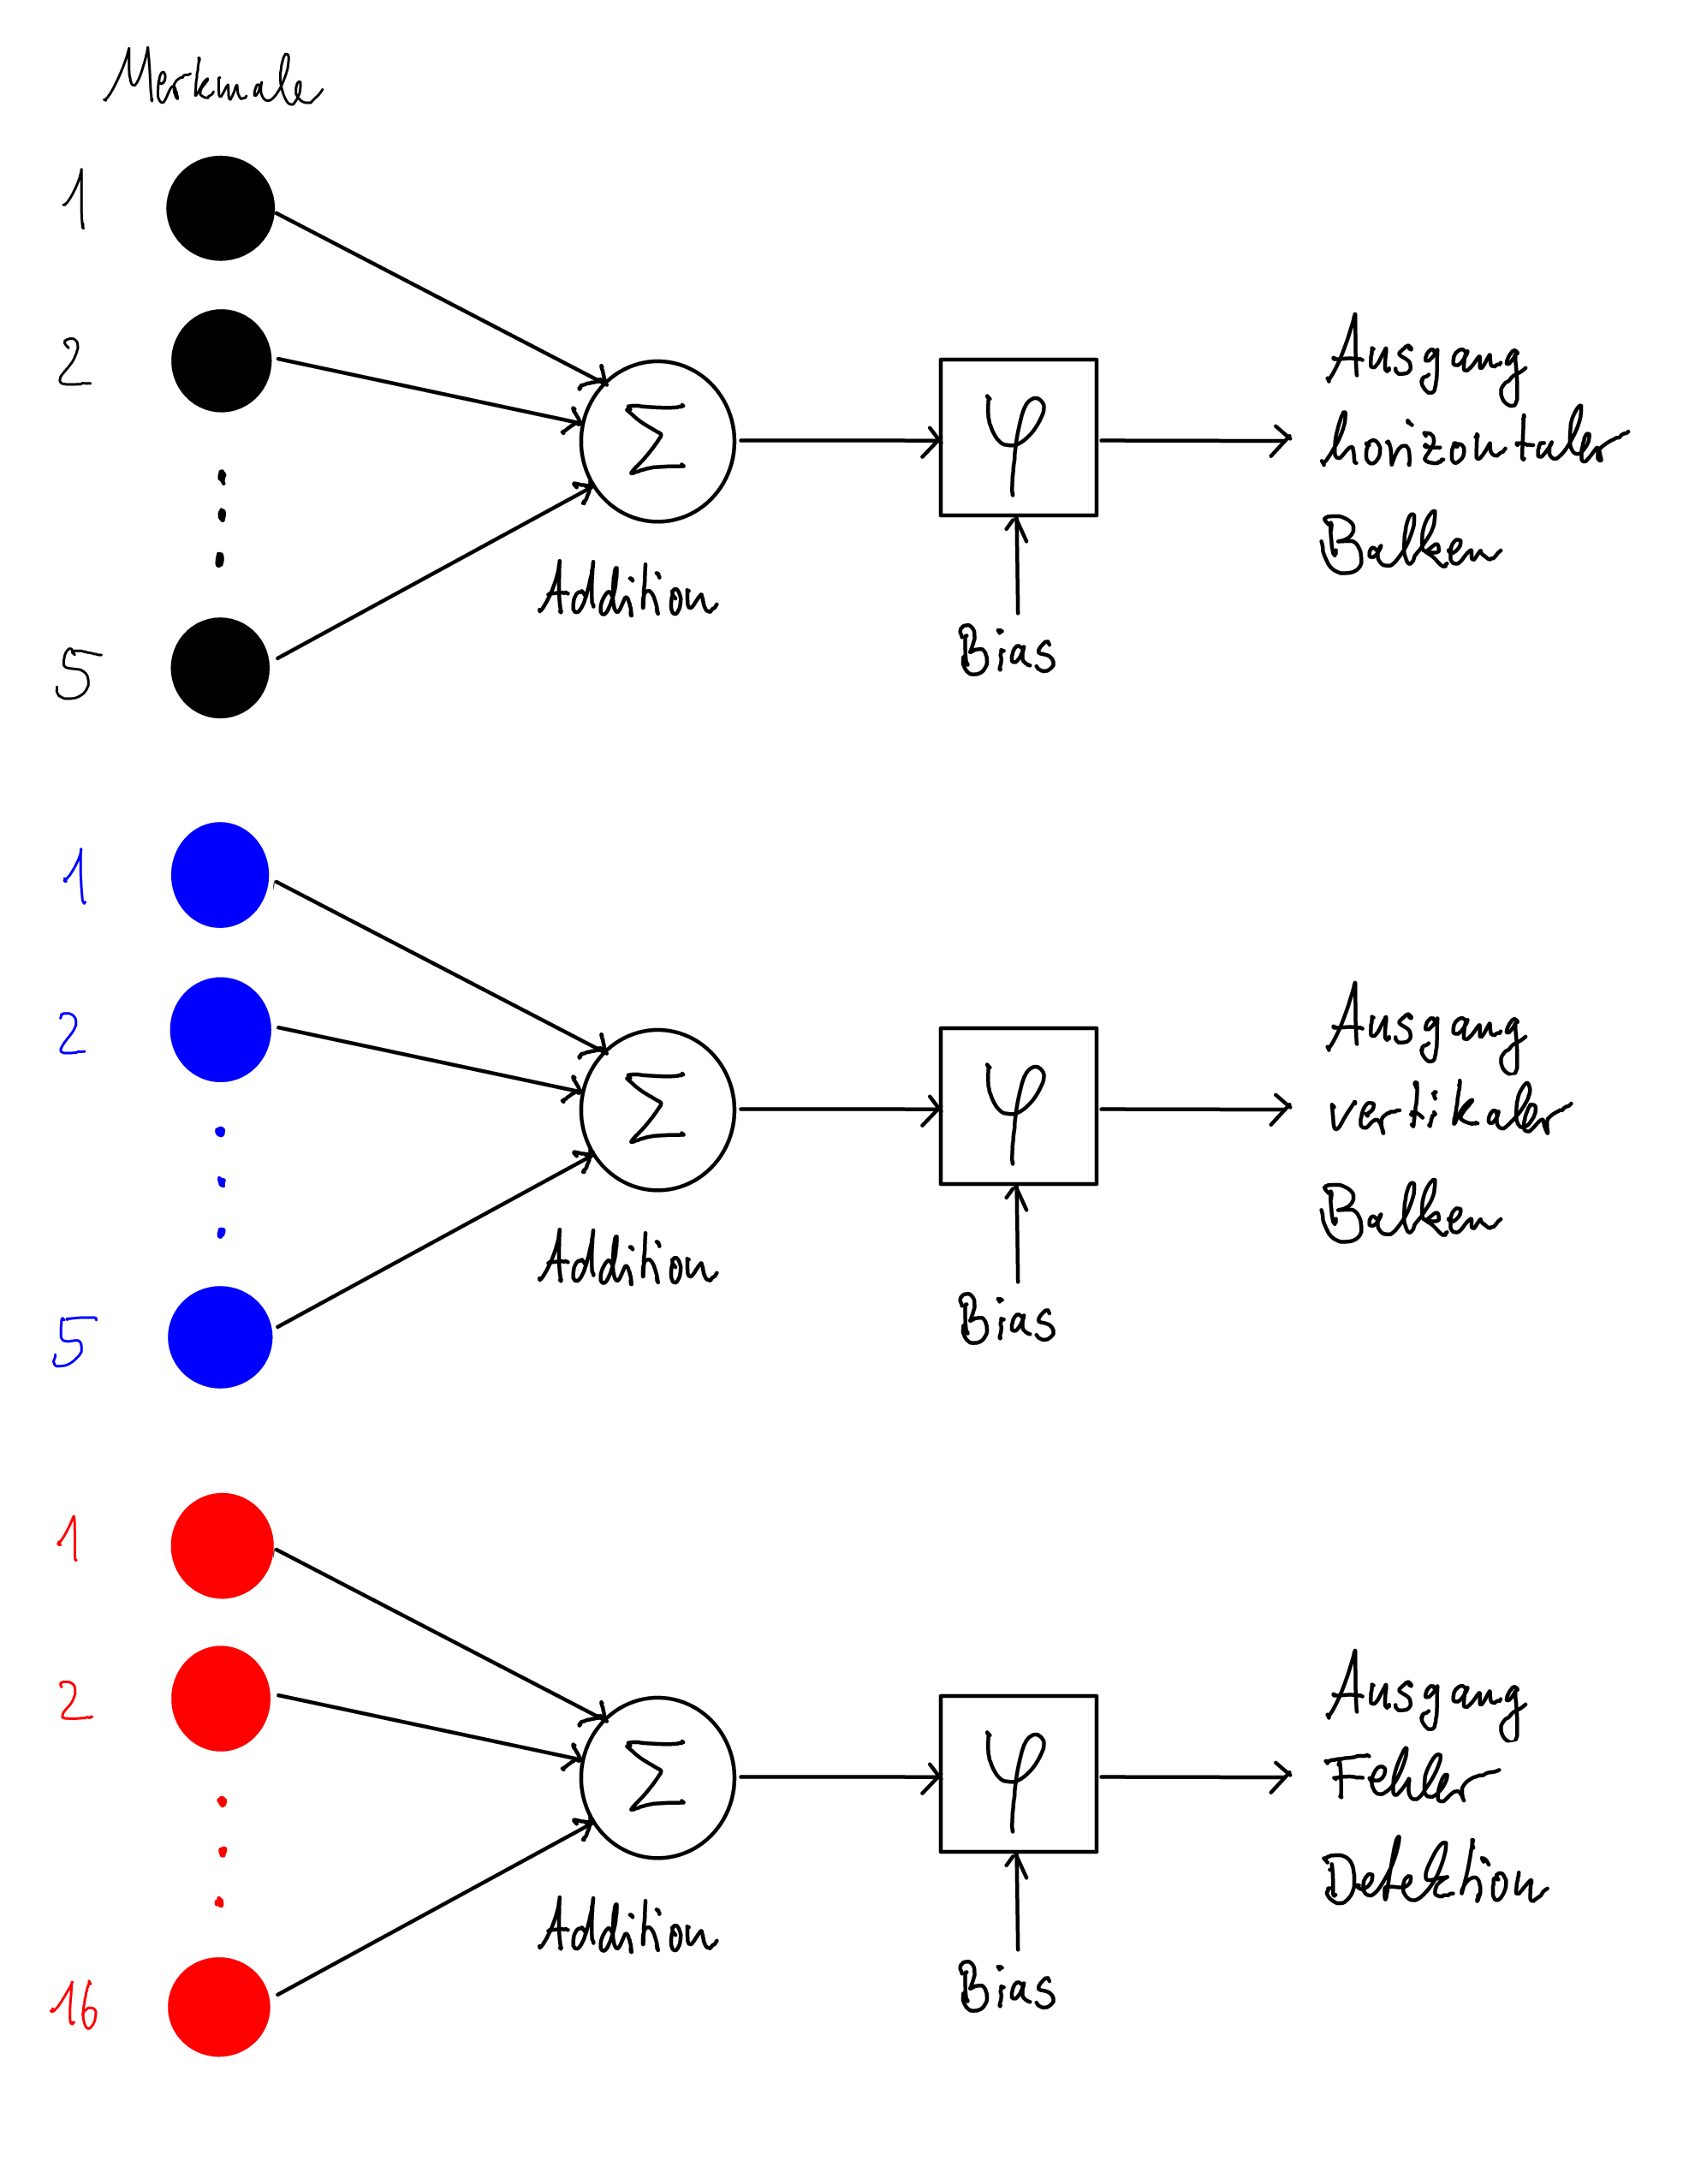
\includegraphics[width=0.8\linewidth]{./Bilder/Auswertung/Aufbau/page7}
	\caption{Neuronen der 2. Ebene}
	\label{Neurin2Ebene}
\end{figure}

Für die Auswertung der Neuronen der erste Ebene nutzen wir eine Sigmoid-Funktion. Für die zweite Ebene werden allerdings nicht die Ergebnisse der Sigmoid-Funktion weitergegeben, sondern die addierten Werte werden ohne eine weiteren Verarbeitung an die zweite Ebene weiter gegeben. Das entspricht einer linearen Aktivierungsfunktion mit dem Anstieg eins.


\section{Erzeugung der Eingangsbilder}

Die Erzeugung von Eingangsbildern für unser neuronales Netz, war eines der ersten Probleme, welches wir gelöst haben. Testbilder zu suchen oder selbst zu erstellen kann sehr zeitaufwendig sein. Aus diesem Grund haben wir zwei Matlab-Skripte geschrieben, die uns dieses Problem zukünftig abnehmen. Die beiden Dateien heißen 'GetPixelFeatureMatrix.m' \ref{GetPixelFeatureMatrix} und 'GetInputFeatureMatrix.m' \ref{GetInputFeatureMatrix}. Die Funktion 'GetPixelFeatureMatrix' erwartet als Eingang eine Merkmale-Matrix, die dann auf eine Pixel-Matrix hochskaliert wird. Darüber hinaus kann auch ein Rauschwert angegeben werden, um das neuronale Netz auf Rauschempfindlichkeit zu testen. Im Anschluss sind ein paar Bilder erzeugt worden. Im Sinne der Lesbarkeit sind im Weiteren alle angebenen Werte für Merkmale, Pixel oder Pixel pro Merkmal lediglich für eine Dimension angegeben, da diese stets symmetrisch sind. Die ersten beiden Abbildungen sollen die Flexibilität der Funktion verdeutlichen und verfügen über 7 Merkmale, 64 Pixel pro Merkmal und einen Rauschanteil von 10\%. Die meisten der nachfolgenden Abbildungen verfügen über fünf Merkmale, 128 Pixel pro Merkmal und somit insgesamt über 640 Pixel und unterscheiden sich neben des dargestellten Musters hauptsächlich in ihrer Rauschintensität. Eine Ausnahme bildet lediglich die Abbildung \ref*{585px9M65pM10} mit 9 Merkmalen, 65 Pixeln pro Merkmal und einem Rauschanteil von 10\%. Somit wird bei den Bildern lediglich die Besonderheiten beziehungsweise der jeweilige Rauschanteil genannt.

\begin{figure}[hbt]
	\begin{minipage}{0.49 \textwidth}
		
\includegraphics[width=\textwidth]{./Bilder/Auswertung/BeispielBilder/Picture_Example4_noise_10_pixelCnt_64_featureCnt_7}
		\caption{Beispielbild 1 mit 10\% Rauschen}
		\label{Toni_Avatar}
	\end{minipage}
	\hfill
	\begin{minipage}{0.49 \textwidth}
		
\includegraphics[width=\textwidth]{./Bilder/Auswertung/BeispielBilder/Picture_Example2_noise_10_pixelCnt_64_featureCnt_7}
		\caption{Beispielbild 2 mit 10\% Rauschen}
		\label{Bryan_Avatar}
	\end{minipage}
\end{figure}

\begin{figure}[hbt]
	\begin{minipage}{0.49 \textwidth}
		
\includegraphics[width=\textwidth]{./Bilder/Auswertung/BeispielBilder/Picture_Crossing_noise_10_pixelCnt_128_featureCnt_5}
		\caption{Kreuz mit 10\% Rauschen}
		% \label{eindeutigerBezeichner}
	\end{minipage}
	\hfill
	\begin{minipage}{0.49 \textwidth}
		
\includegraphics[width=\textwidth]{./Bilder/Auswertung/BeispielBilder/Picture_Crossing_noise_10_pixelCnt_65_featureCnt_9}
		\caption{Kreuz mit 9 Merkmalen und 10\% Rauschen}
		\label{585px9M65pM10}
	\end{minipage}
\end{figure}

\begin{figure}[hbt]
	\begin{minipage}{0.49 \textwidth}
		
\includegraphics[width=\textwidth]{./Bilder/Auswertung/BeispielBilder/Picture_Line1_noise_10_pixelCnt_128_featureCnt_5}
		\caption{Horizontaler Balken mit 10\% Rauschen}
		% \label{eindeutigerBezeichner}
	\end{minipage}
	\hfill
	\begin{minipage}{0.49 \textwidth}
		
\includegraphics[width=\textwidth]{./Bilder/Auswertung/BeispielBilder/Picture_Line2_noise_10_pixelCnt_128_featureCnt_5}
		\caption{Diagonale mit 10\% Rauschen}
		% \label{eindeutigerBezeichner}
	\end{minipage}
\end{figure}

\begin{figure}[hbt]
	\begin{minipage}{0.49 \textwidth}
		
\includegraphics[width=\textwidth]{./Bilder/Auswertung/BeispielBilder/Picture_Crossing_noise_0_pixelCnt_128_featureCnt_5}
		\caption{Kreuz ohne Rauschen}
		% \label{eindeutigerBezeichner}
	\end{minipage}
	\hfill
	\begin{minipage}{0.49 \textwidth}
		
\includegraphics[width=\textwidth]{./Bilder/Auswertung/BeispielBilder/Picture_Crossing_noise_20_pixelCnt_128_featureCnt_5}
		\caption{Kreuz mit 20\% Rauschen}
		% \label{eindeutigerBezeichner}
	\end{minipage}
\end{figure}

\begin{figure}[hbt]
	\begin{minipage}{0.49 \textwidth}
		
\includegraphics[width=\textwidth]{./Bilder/Auswertung/BeispielBilder/Picture_Crossing_noise_30_pixelCnt_128_featureCnt_5}
		\caption{Kreuz mit 30\% Rauschen}
		% \label{eindeutigerBezeichner}
	\end{minipage}
	\hfill
	\begin{minipage}{0.49 \textwidth}
		
\includegraphics[width=\textwidth]{./Bilder/Auswertung/BeispielBilder/Picture_Crossing_noise_40_pixelCnt_128_featureCnt_5}
		\caption{Kreuz mit 40\% Rauschen}
		% \label{eindeutigerBezeichner}
	\end{minipage}
\end{figure}

\begin{figure}[hbt]
	\begin{minipage}{0.49 \textwidth}
		
\includegraphics[width=\textwidth]{./Bilder/Auswertung/BeispielBilder/Picture_Crossing_noise_50_pixelCnt_128_featureCnt_5}
		\caption{Kreuz mit 50\% Rauschen}
		% \label{eindeutigerBezeichner}
	\end{minipage}
	\hfill
	\begin{minipage}{0.49 \textwidth}
		
\includegraphics[width=\textwidth]{./Bilder/Auswertung/BeispielBilder/Picture_Crossing_noise_60_pixelCnt_128_featureCnt_5}
		\caption{Kreuz mit 60\% Rauschen}
		% \label{eindeutigerBezeichner}
	\end{minipage}
\end{figure}

\begin{figure}[hbt]
	\begin{minipage}{0.49 \textwidth}
		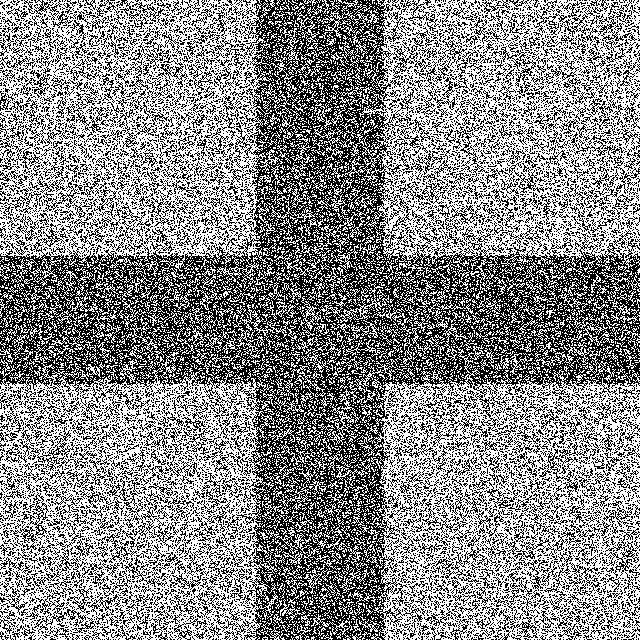
\includegraphics[width=\textwidth]{./Bilder/Auswertung/BeispielBilder/Picture_Crossing_noise_70_pixelCnt_128_featureCnt_5}
		\caption{Kreuz mit 70\% Rauschen}
		% \label{eindeutigerBezeichner}
	\end{minipage}
	\hfill
	\begin{minipage}{0.49 \textwidth}
		
\includegraphics[width=\textwidth]{./Bilder/Auswertung/BeispielBilder/Picture_Crossing_noise_80_pixelCnt_128_featureCnt_5}
		\caption{Kreuz mit 80\% Rauschen}
		% \label{eindeutigerBezeichner}
	\end{minipage}
\end{figure}

\begin{figure}[hbt]
	\begin{minipage}{0.49 \textwidth}
		
\includegraphics[width=\textwidth]{./Bilder/Auswertung/BeispielBilder/Picture_Crossing_noise_90_pixelCnt_128_featureCnt_5}
		\caption{Kreuz mit 90\% Rauschen}
		% \label{eindeutigerBezeichner}
	\end{minipage}
	\hfill
	\begin{minipage}{0.49 \textwidth}
		
\includegraphics[width=\textwidth]{./Bilder/Auswertung/BeispielBilder/Picture_Crossing_noise_100_pixelCnt_128_featureCnt_5}
		\caption{Kreuz mit 100\% Rauschen}
		% \label{eindeutigerBezeichner}
	\end{minipage}
\end{figure}

\begin{figure}[hbt]
	\centering
	
\includegraphics[width=0.7\linewidth]{./Bilder/Auswertung/BeispielBilder/Picture_Example1_noise_10_pixelCnt_128_featureCnt_5}
	\caption{Schachbrettmuster mit 10\% Rauschen}
	% \label{eindeutigerBezeichner}
\end{figure}
\section{Gewichtsmatrizen} \label{gewichtsmatrizenSection}
In diesem Abschnitt werden verschiedene Gewichtsmatrizen vorgestellt und wie wir sie erzeugt haben. Wir haben uns erst einmal auf die Erzeugung mit der Gauß-Funktion konzentriert. Es sind auch andere Funktionen möglich, wie zum Beispiel die Rayleigh-Funktion. Aus zeitlichen Gründen mussten wie darauf leider verzichten.

Zuerst soll gezeigt werden, wie die Gewichtsmatrizen grob erstellt wurden. Dafür werden im Abschnitt \ref{eGew} 3 Beispiele mit jeweils einem Slope von 75 gezeigt. Es soll außerdem verdeutlicht werden, dass es sich immer nur um einen Gauß in x- und y-Richtung handelt. Des Weiteren ist das Endergebnis immer zwischen -1 und 1. So können wir später den Ergebnisbereich besser skalieren.

In den anderen Unter-Abschnitten sind für jede Art der Gewichtsmatrizen verschiedene Slopes eingestellt.

\newpage
\subsection{Erzeugung der Gewichtsmatrizen} \label{eGew}
\begin{figure}[hbt]
	\centering
	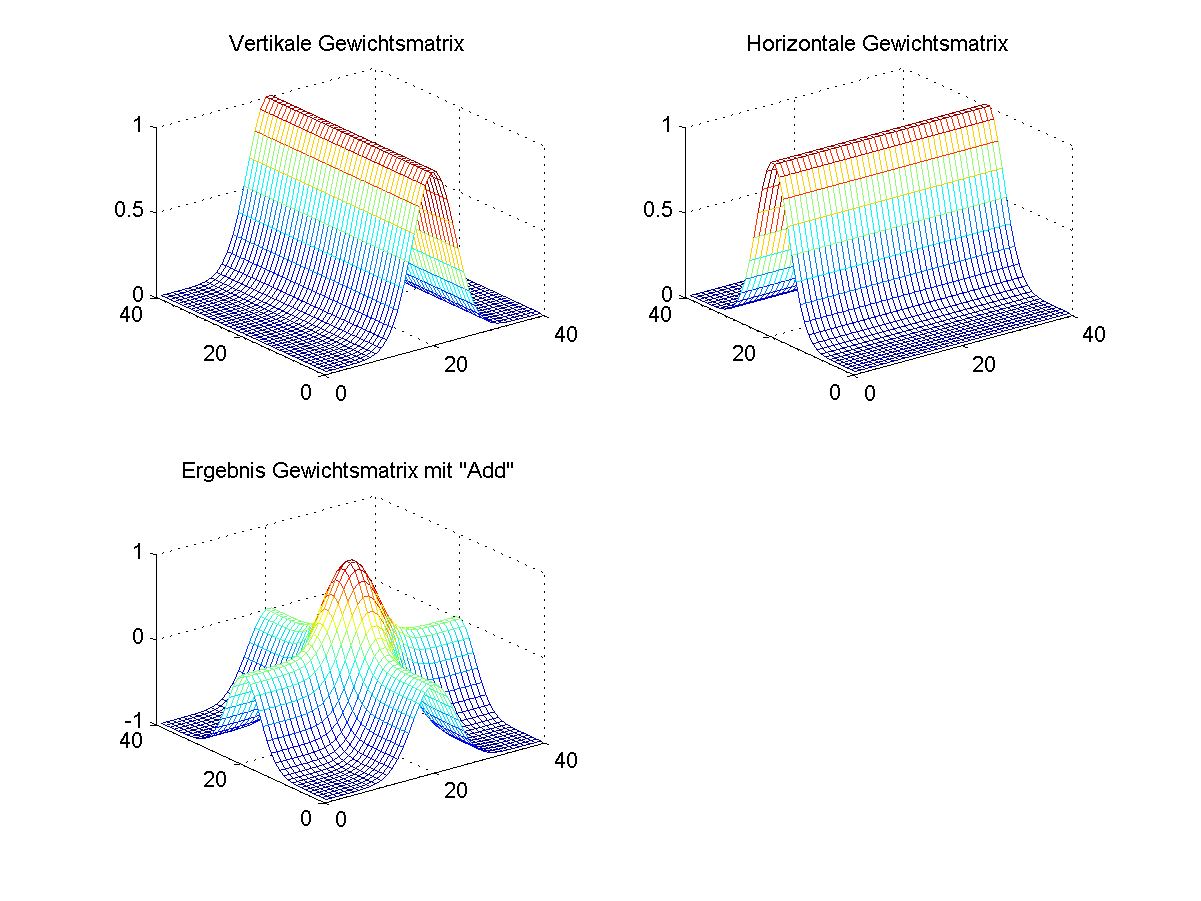
\includegraphics[width=1\linewidth]{./Bilder/Auswertung/GewichtmatrixEinzelschritte/Endergebnis_Gewichtsmatrix_Slope_75_Type_Add}
	\caption{Additive Überlagerung mit Slope von 75}
	\label{Add75}
\end{figure}

\begin{lstlisting}[label=code:Add75, caption=Auszug Matlab-Skript 'GetGaussWeights()']
elseif strcmp(type, 'Add')
	for i = 1:vN
		tempWeightMatrix(1:end, i) = (vWeightMatrix(1:end, i) + (hGauss./max(hGauss))')./2;
		tempWeightMatrix(1:end, i) = tempWeightMatrix(1:end, i) .* 2 - 1;
	end
\end{lstlisting}

In Abbildung \ref{Add75} wurde der 3D-Gauß in x- und y-Richtung additiv Überlagert, mit 2 multipliziert und am Ende um 1 heruntergesetzt. Siehe auch das Listing \ref{code:Add75}.

\newpage
\begin{figure}[hbt]
	\centering
	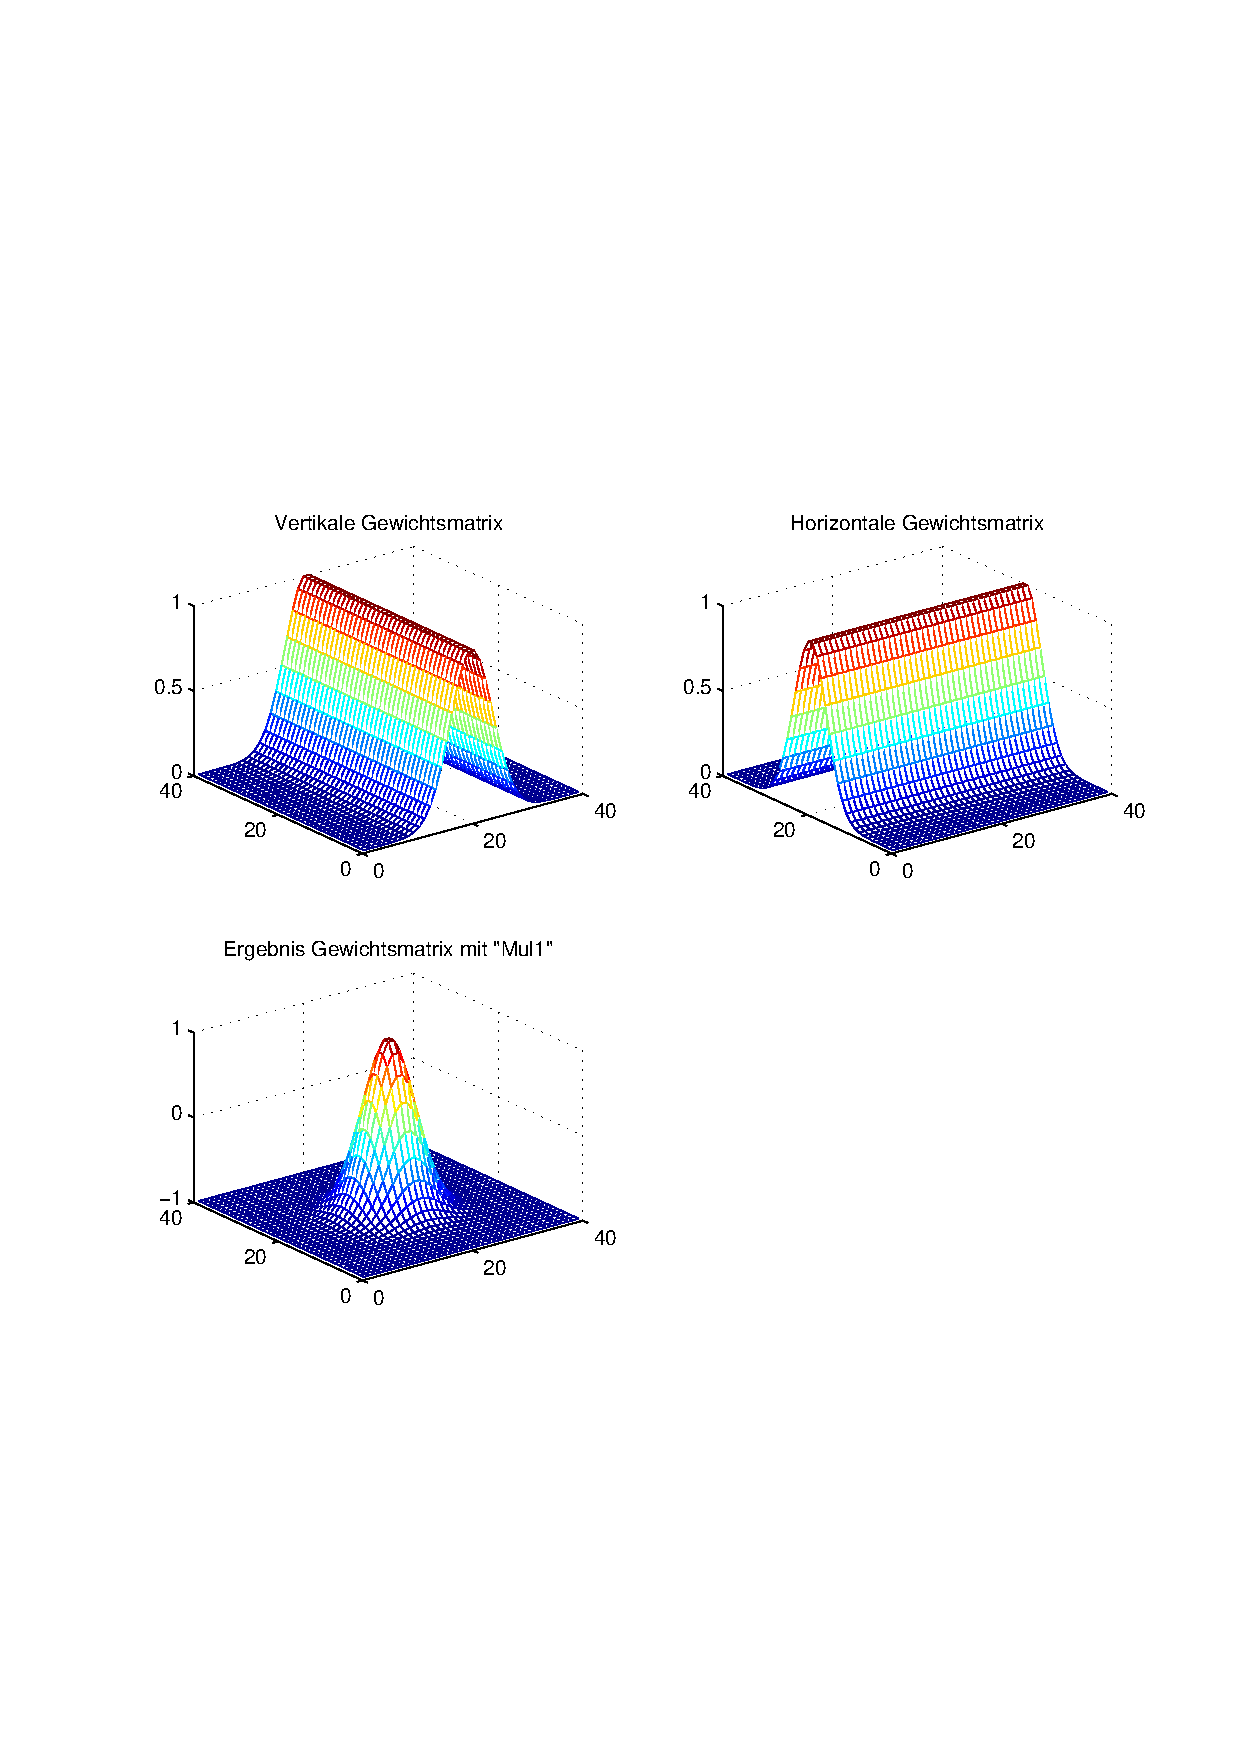
\includegraphics[width=1\linewidth]{./Bilder/Auswertung/GewichtmatrixEinzelschritte/Endergebnis_Gewichtsmatrix_Slope_75_Type_Mul1}
	\caption{Multiplikative Überlagerung Typ 1 mit Slope von 75}
	\label{Mul175}
\end{figure}

\begin{lstlisting}[label=code:Mul175, caption=Auszug Matlab-Skript 'GetGaussWeights()']
if strcmp(type, 'Mul1')
	for i = 1:vN
		tempWeightMatrix(1:end, i) = vWeightMatrix(1:end, i) .* (hGauss./max(hGauss))';
		tempWeightMatrix(1:end, i) = tempWeightMatrix(1:end, i) .* 2 - 1;
	end
\end{lstlisting}

In Abbildung \ref{Mul175} wurde der 3D-Gauß in x- und y-Richtung multiplikativ Überlagert, mit 2 multipliziert und am Ende um 1 heruntergesetzt. Siehe auch das Listing \ref{code:Mul175}.

\newpage
\begin{figure}[hbt]
	\centering
	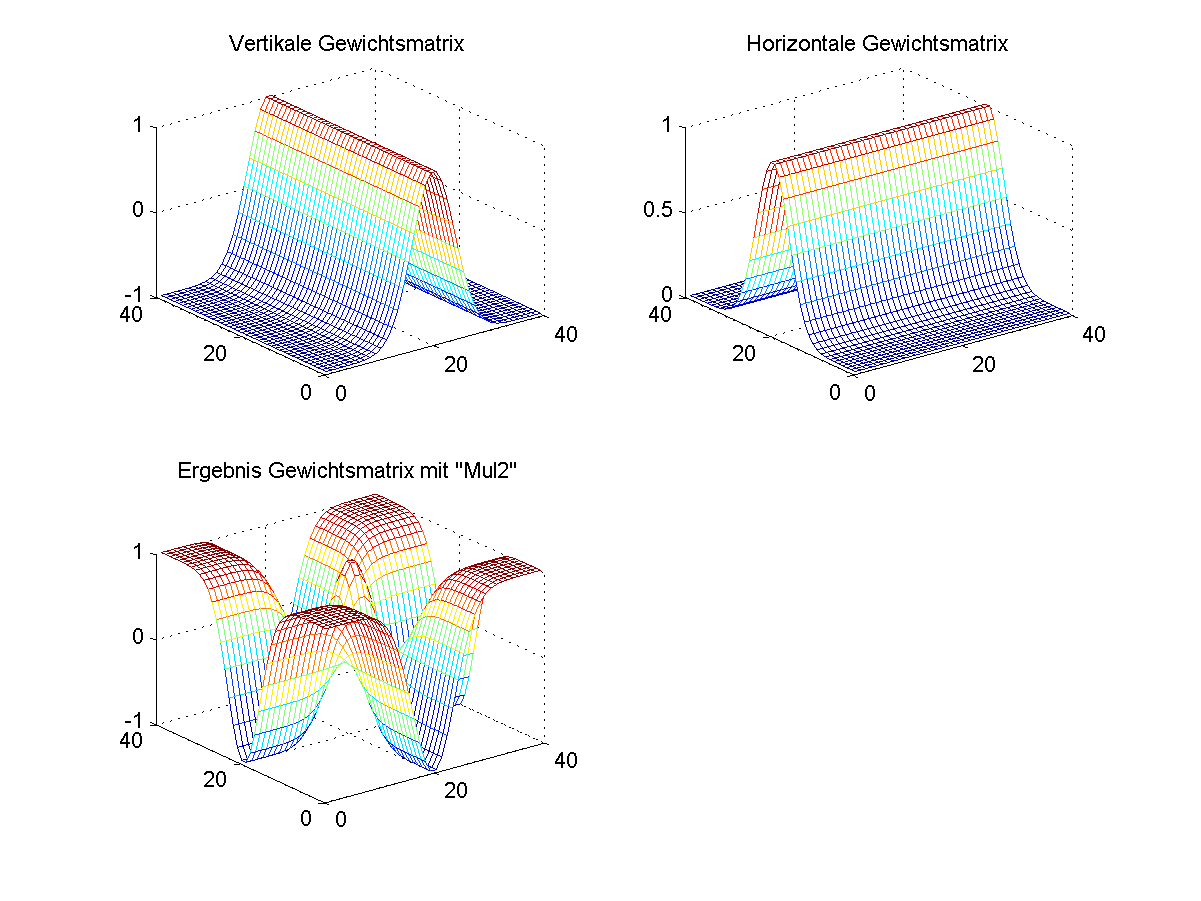
\includegraphics[width=1\linewidth]{./Bilder/Auswertung/GewichtmatrixEinzelschritte/Endergebnis_Gewichtsmatrix_Slope_75_Type_Mul2}
	\caption{Multiplikative Überlagerung Typ 2 mit Slope von 75}
	\label{Mul275}
\end{figure}

\begin{lstlisting}[label=code:Mul275, caption=Auszug Matlab-Skript 'GetGaussWeights()']
elseif strcmp(type, 'Mul2')
	for i = 1:vN
		% skalieren auf -1 bis 1
		vWeightMatrix(1:end, i) = vWeightMatrix(1:end, i) .* 2 - 1;
		% v-Gauss und h-Gauss multiplizieren
		tempWeightMatrix(1:end, i) = vWeightMatrix(1:end, i) .* ((hGauss./max(hGauss)) * 2 - 1)';
	end
\end{lstlisting}

In Abbildung \ref{Mul275} wurde der 3D-Gauß in der einen y-Richtung erst einmal zwischen -1 und 1 skaliert. Anschließend wird der 3D-Gauß in x-Richtung ebenfalls zwischen -1 und 1 skaliert. Am Ende werden beide multiplikativ überlagert. Siehe auch das Listing \ref{code:Mul275}.

\newpage
\subsection{Additive Überlagerung}
\begin{figure}[hbt]
	\begin{minipage}{0.5 \textwidth}
		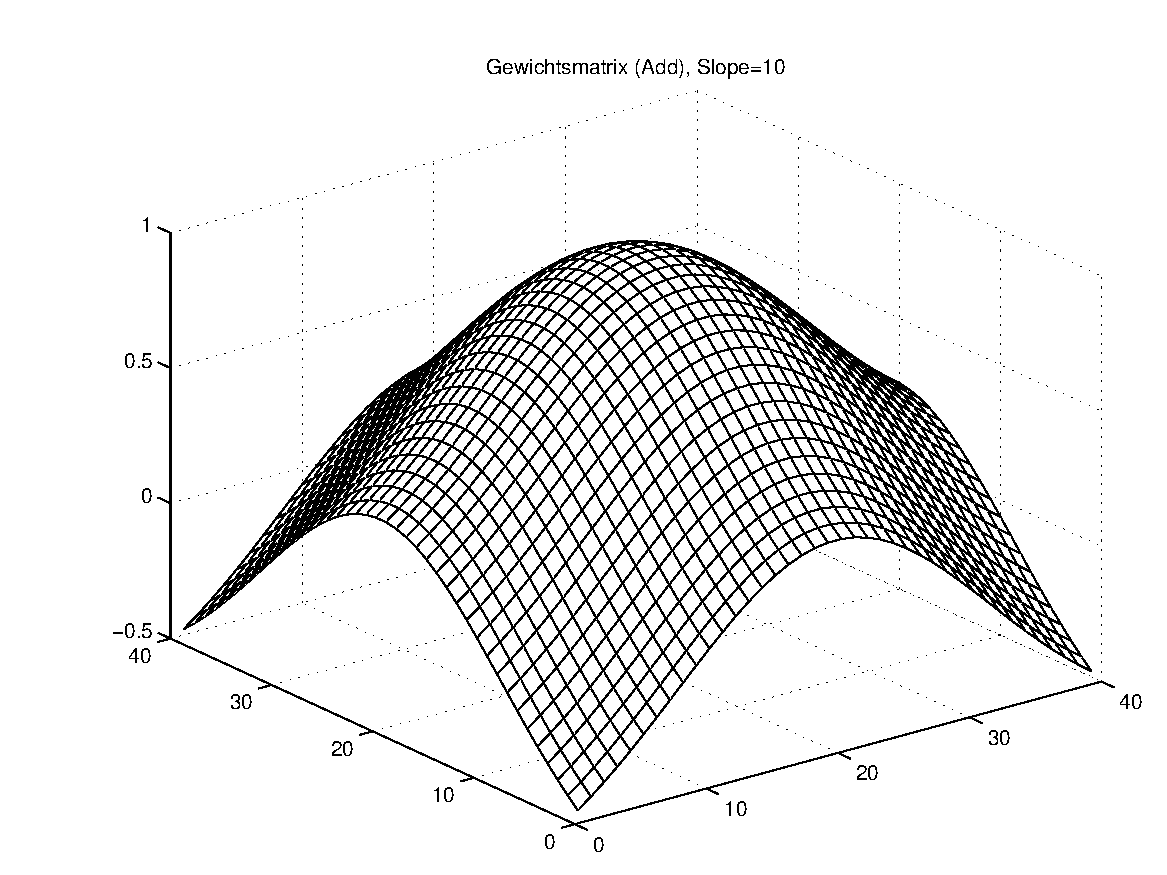
\includegraphics[width=\textwidth]{./Bilder/Auswertung/Gewichtsmatrix/Gewichtsmatrix_Add_Slope_10}
		\caption{Additive Überlagerung mit Slope von 10}
		\label{Add10}
	\end{minipage}
	\hfill
	\begin{minipage}{0.5 \textwidth}
		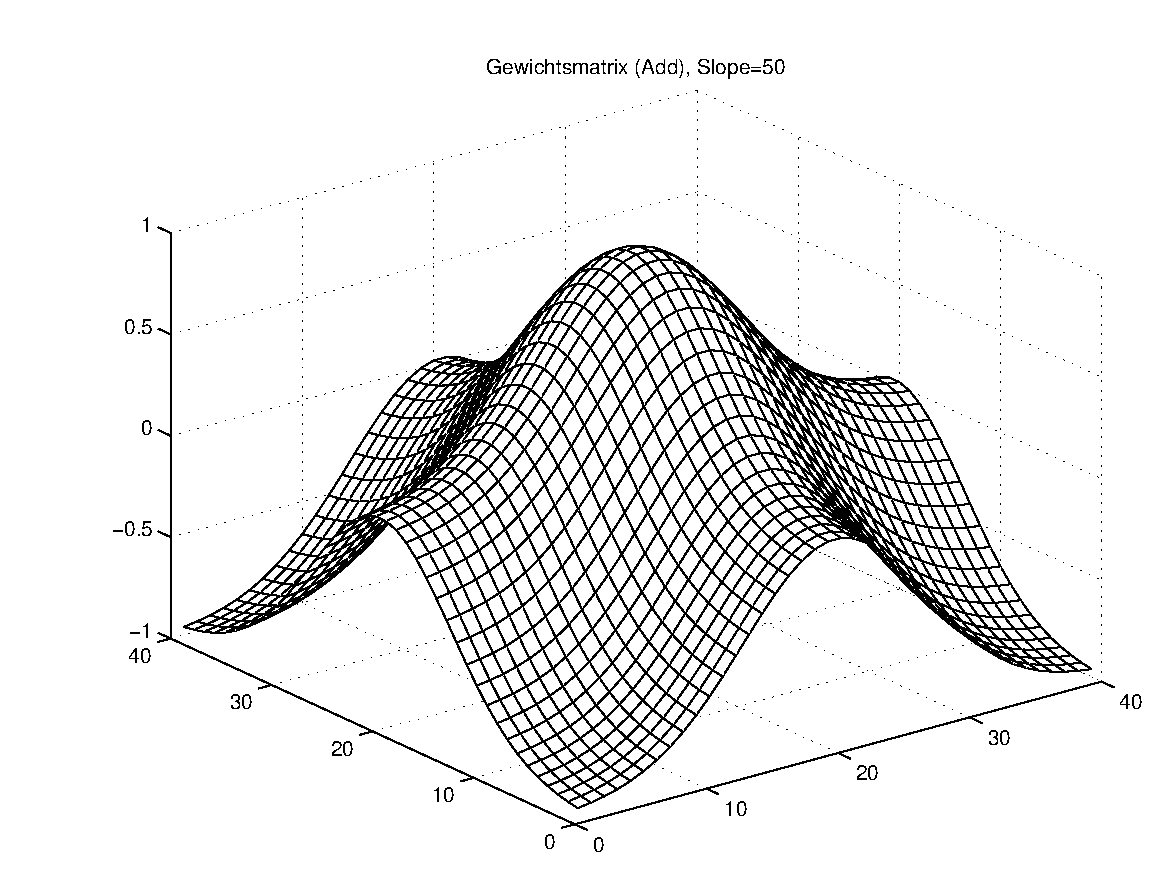
\includegraphics[width=\textwidth]{./Bilder/Auswertung/Gewichtsmatrix/Gewichtsmatrix_Add_Slope_50}
		\caption{Additive Überlagerung mit Slope von 50}
		\label{Add50}
	\end{minipage}
\end{figure}

\begin{figure}[hbt]
	\centering
	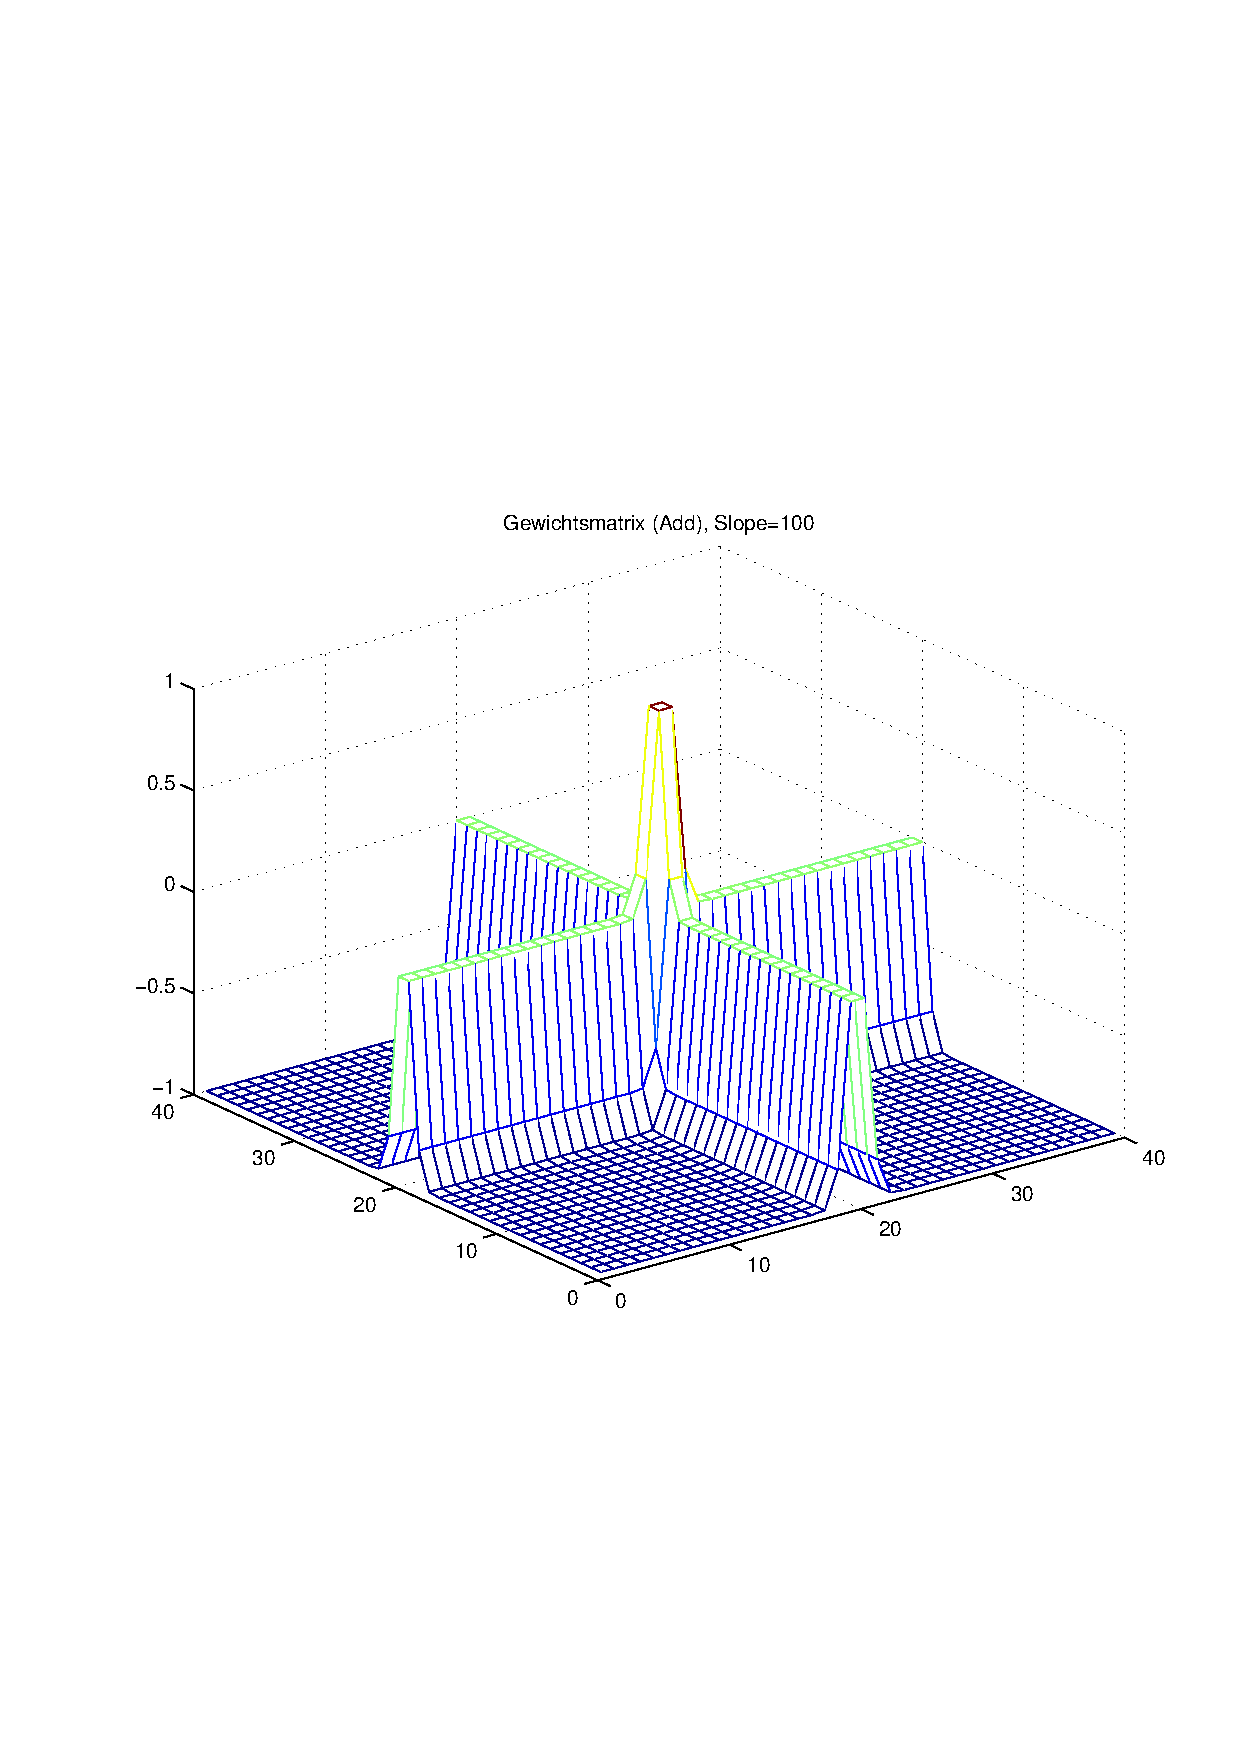
\includegraphics[width=0.6\linewidth]{./Bilder/Auswertung/Gewichtsmatrix/Gewichtsmatrix_Add_Slope_100}
	\caption{Additive Überlagerung mit Slope von 100}
	\label{Add100}
\end{figure}

\newpage
\subsection{Multiplikative Überlagerung Typ 1}
\begin{figure}[hbt]
	\begin{minipage}{0.5 \textwidth}
		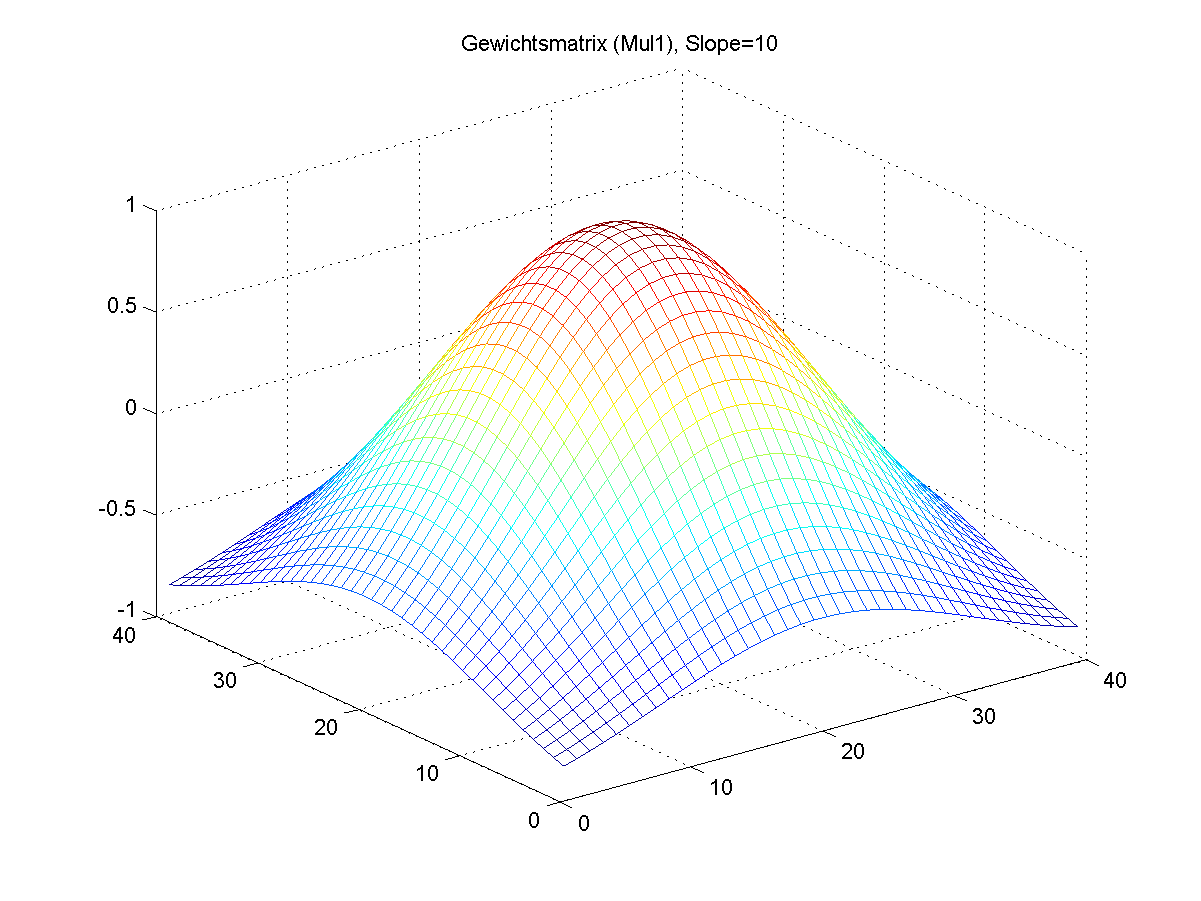
\includegraphics[width=\textwidth]{./Bilder/Auswertung/Gewichtsmatrix/Gewichtsmatrix_Mul1_Slope_10}
		\caption{Multiplikative Überlagerung Typ 1 mit Slope von 10}
		\label{Mul110}
	\end{minipage}
	\hfill
	\begin{minipage}{0.5 \textwidth}
		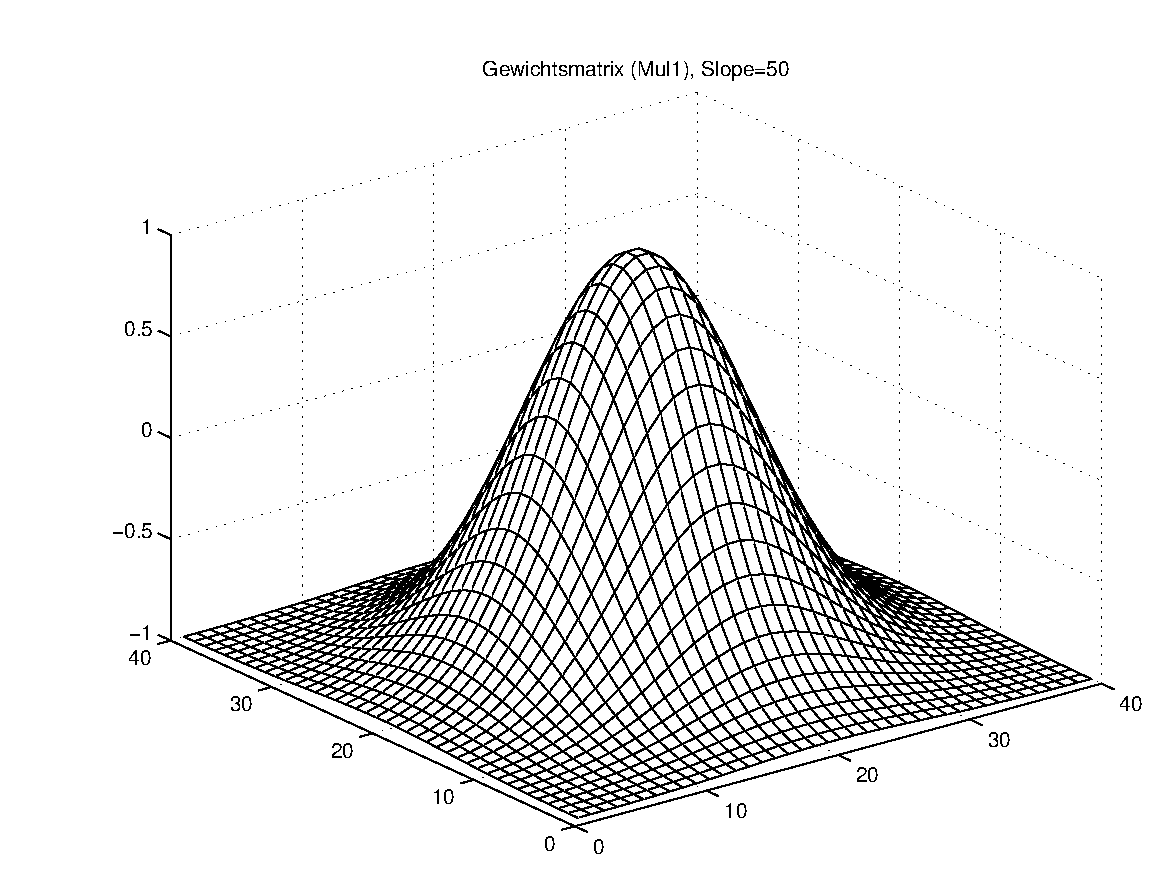
\includegraphics[width=\textwidth]{./Bilder/Auswertung/Gewichtsmatrix/Gewichtsmatrix_Mul1_Slope_50}
		\caption{Multiplikative Überlagerung Typ 1 mit Slope von 50}
		\label{Mul150}
	\end{minipage}
\end{figure}

\begin{figure}[hbt]
	\centering
	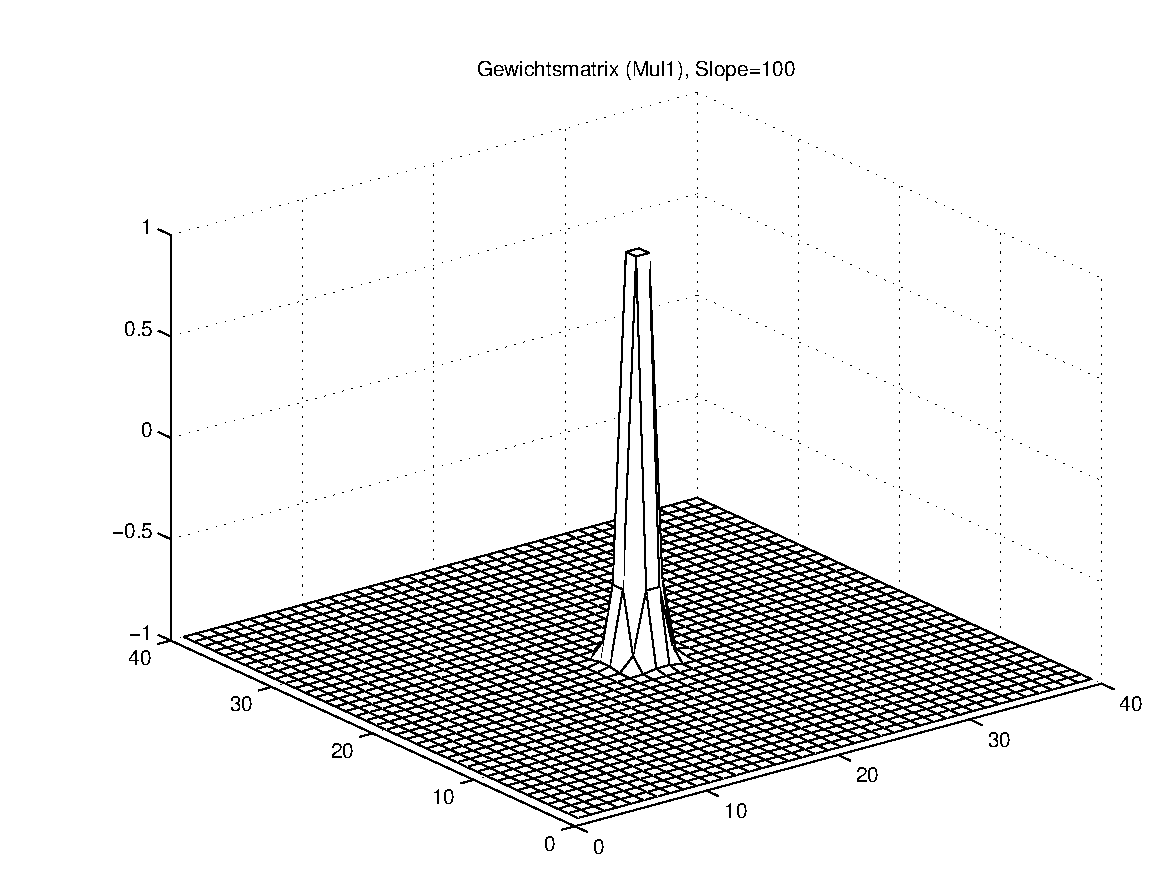
\includegraphics[width=0.6\linewidth]{./Bilder/Auswertung/Gewichtsmatrix/Gewichtsmatrix_Mul1_Slope_100}
	\caption{Multiplikative Überlagerung Typ 1 mit Slope von 100}
	\label{Mul1100}
\end{figure}

\newpage
\subsection{Multiplikative Überlagerung Typ 2}
\begin{figure}[hbt]
	\begin{minipage}{0.5 \textwidth}
		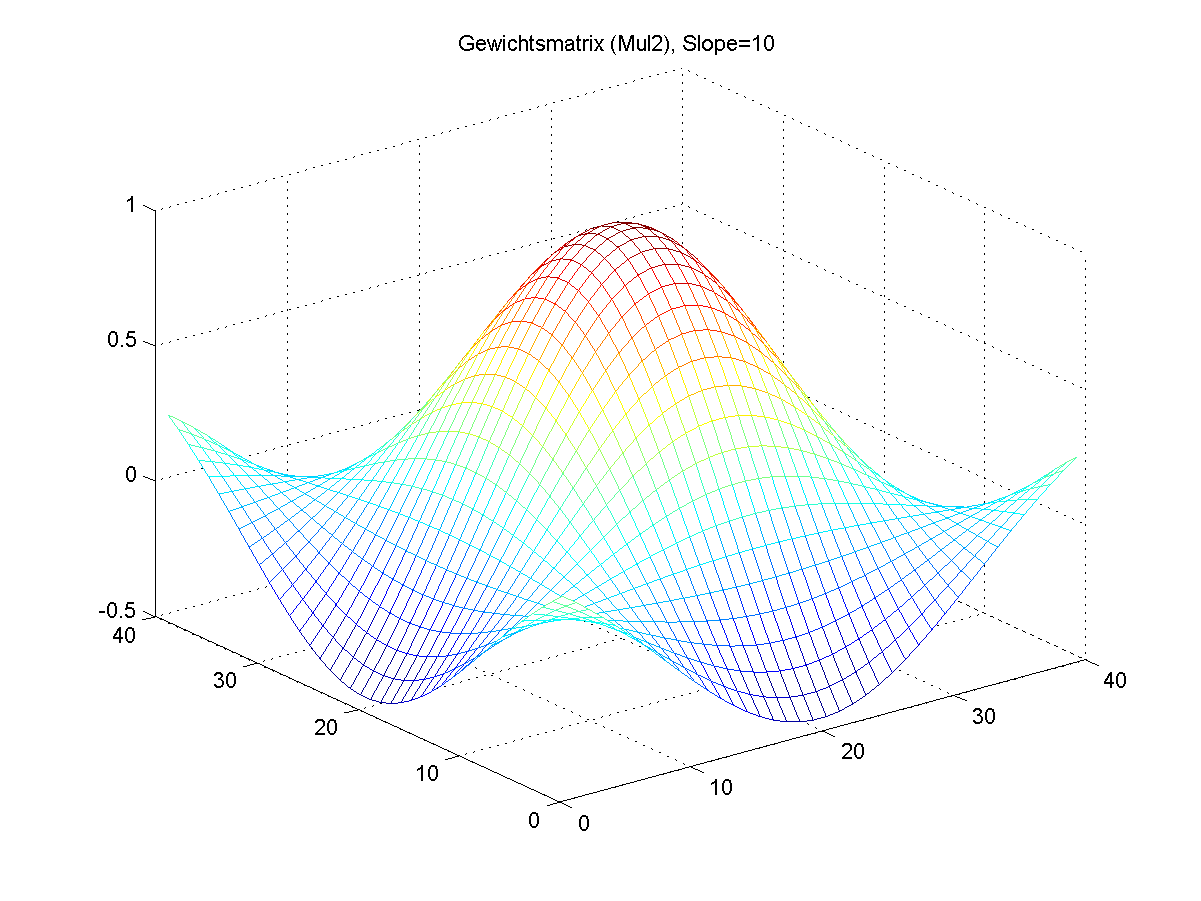
\includegraphics[width=\textwidth]{./Bilder/Auswertung/Gewichtsmatrix/Gewichtsmatrix_Mul2_Slope_10}
		\caption{Multiplikative Überlagerung Typ 2 mit Slope von 10}
		\label{Mul210}
	\end{minipage}
	\hfill
	\begin{minipage}{0.5 \textwidth}
		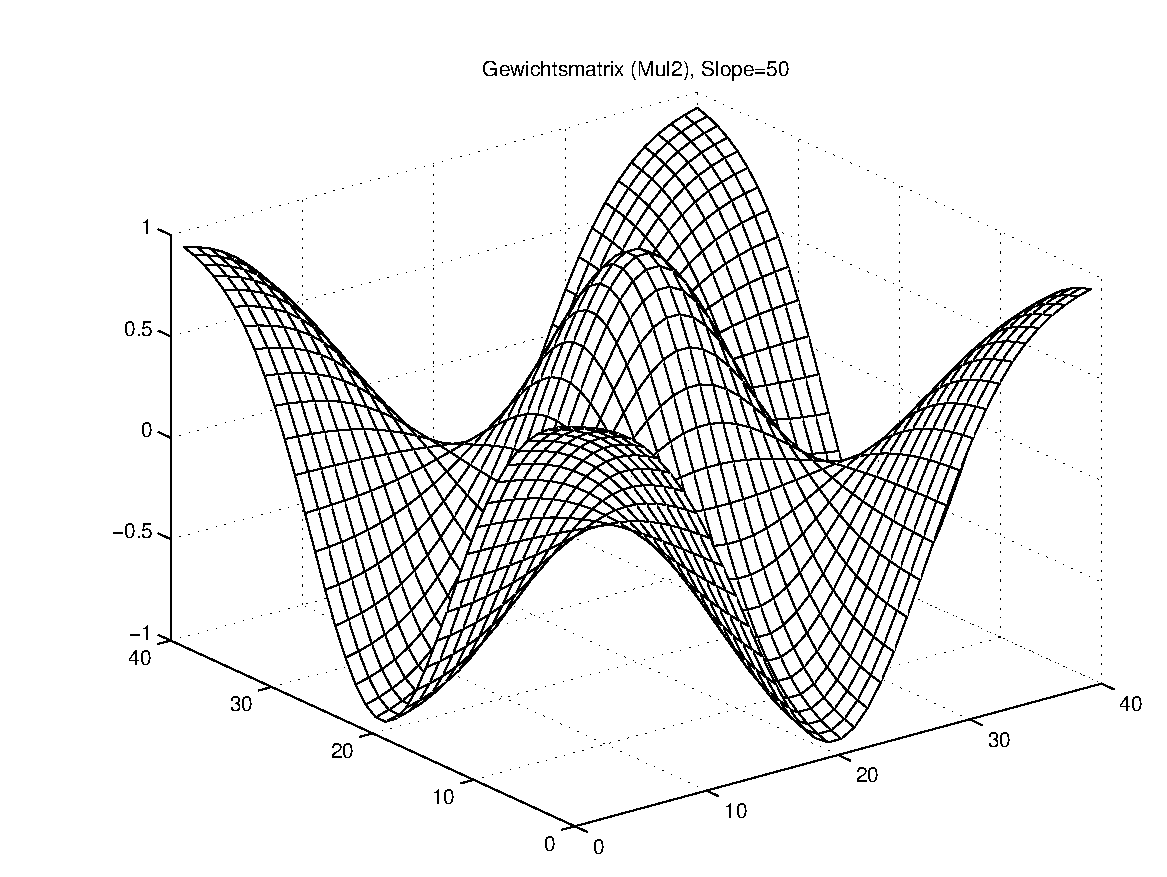
\includegraphics[width=\textwidth]{./Bilder/Auswertung/Gewichtsmatrix/Gewichtsmatrix_Mul2_Slope_50}
		\caption{Multiplikative Überlagerung Typ 2 mit Slope von 50}
		\label{Mul250}
	\end{minipage}
\end{figure}

\begin{figure}[hbt]
	\centering
	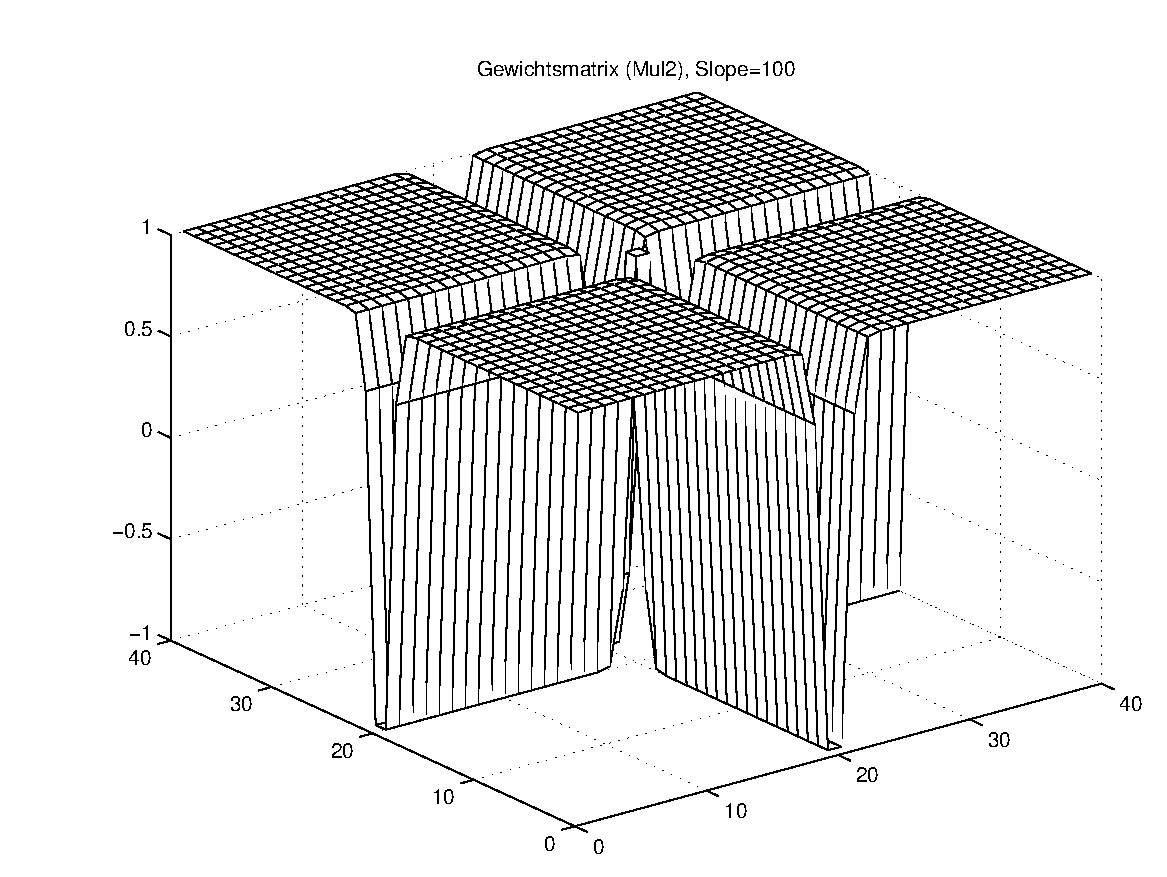
\includegraphics[width=0.6\linewidth]{./Bilder/Auswertung/Gewichtsmatrix/Gewichtsmatrix_Mul2_Slope_100}
	\caption{Multiplikative Überlagerung Typ 2 mit Slope von 100}
	\label{Mul2100}
\end{figure}


\newpage
\subsection{Additive und Multiplikative Überlagerung}
\begin{figure}[hbt]
	\begin{minipage}{0.5 \textwidth}
		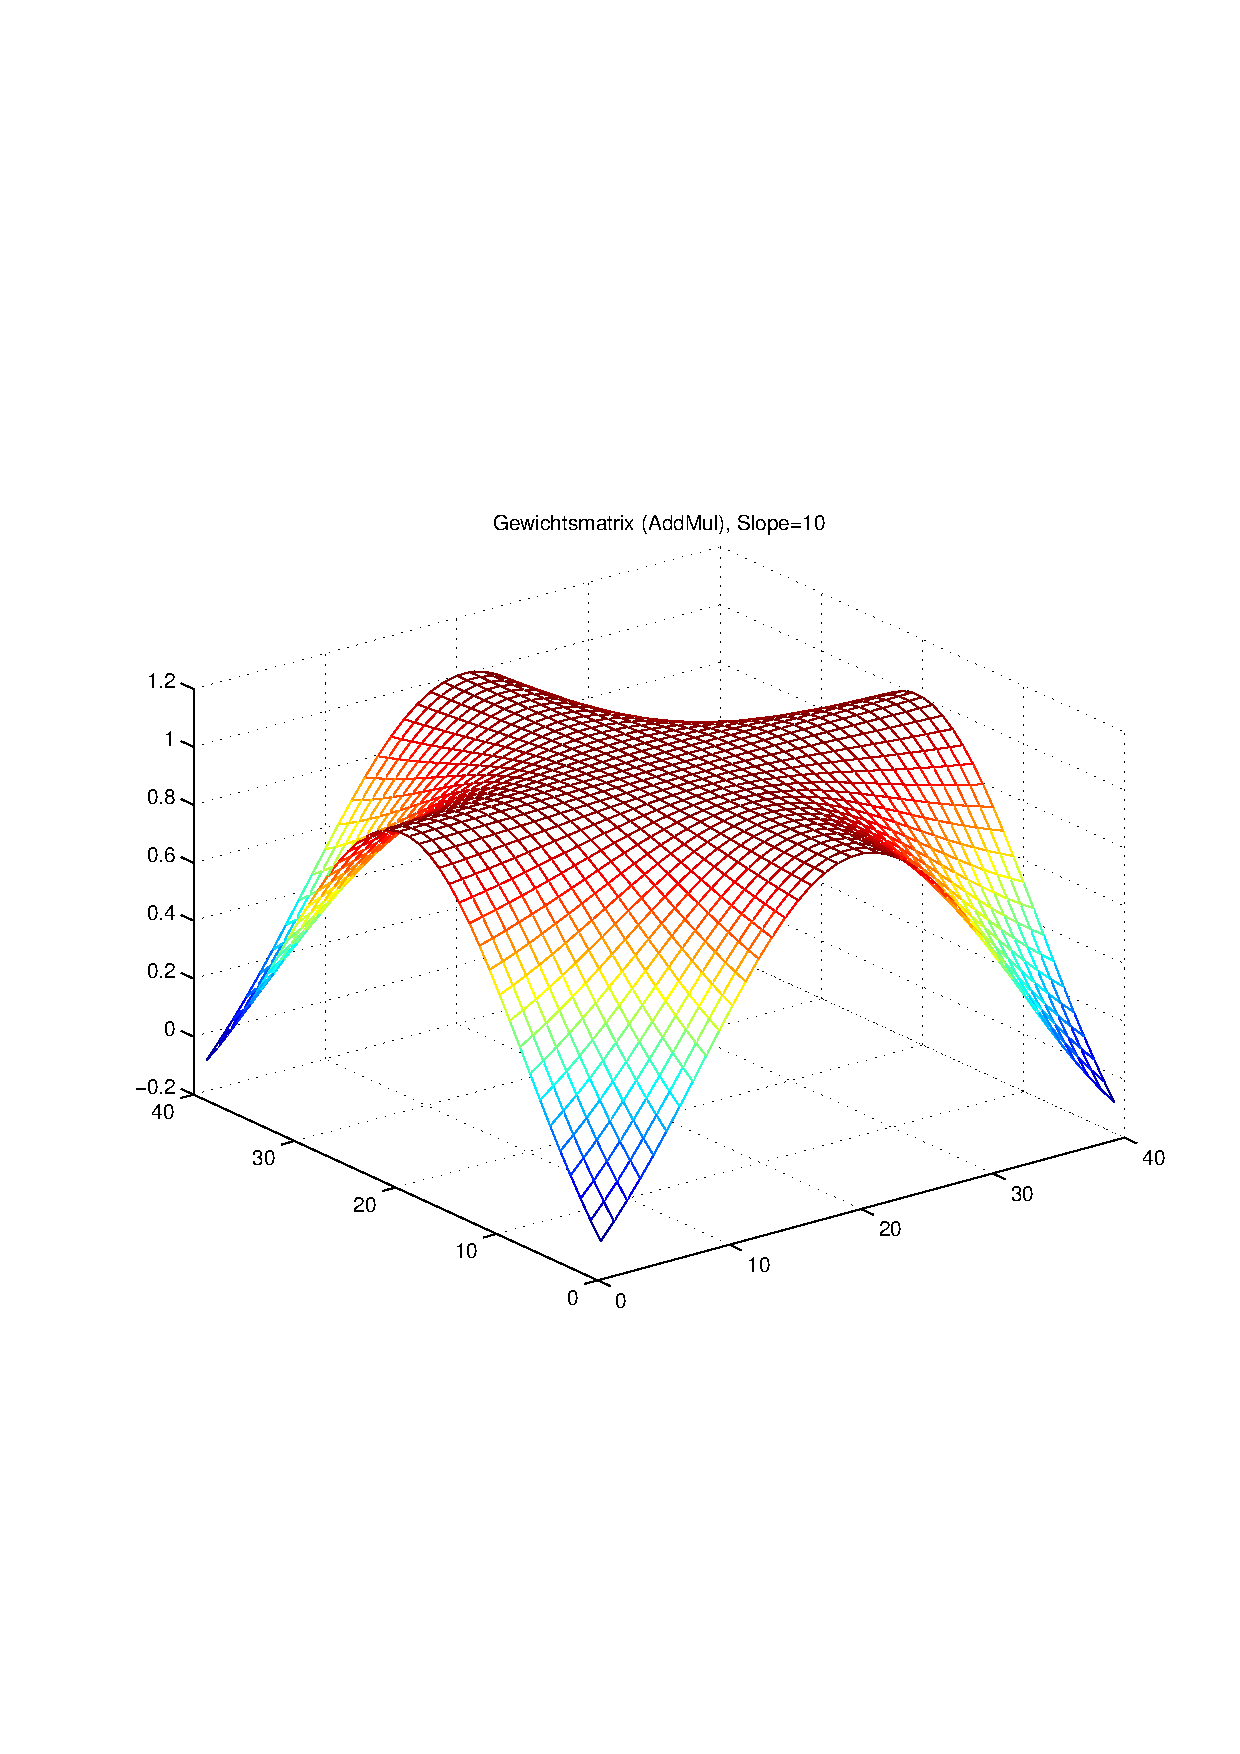
\includegraphics[width=\textwidth]{./Bilder/Auswertung/Gewichtsmatrix/Gewichtsmatrix_AddMul_Slope_10}
		\caption{Additive und Multiplikative Überlagerung mit Slope von 10}
		\label{AddMul210}
	\end{minipage}
	\hfill
	\begin{minipage}{0.5 \textwidth}
		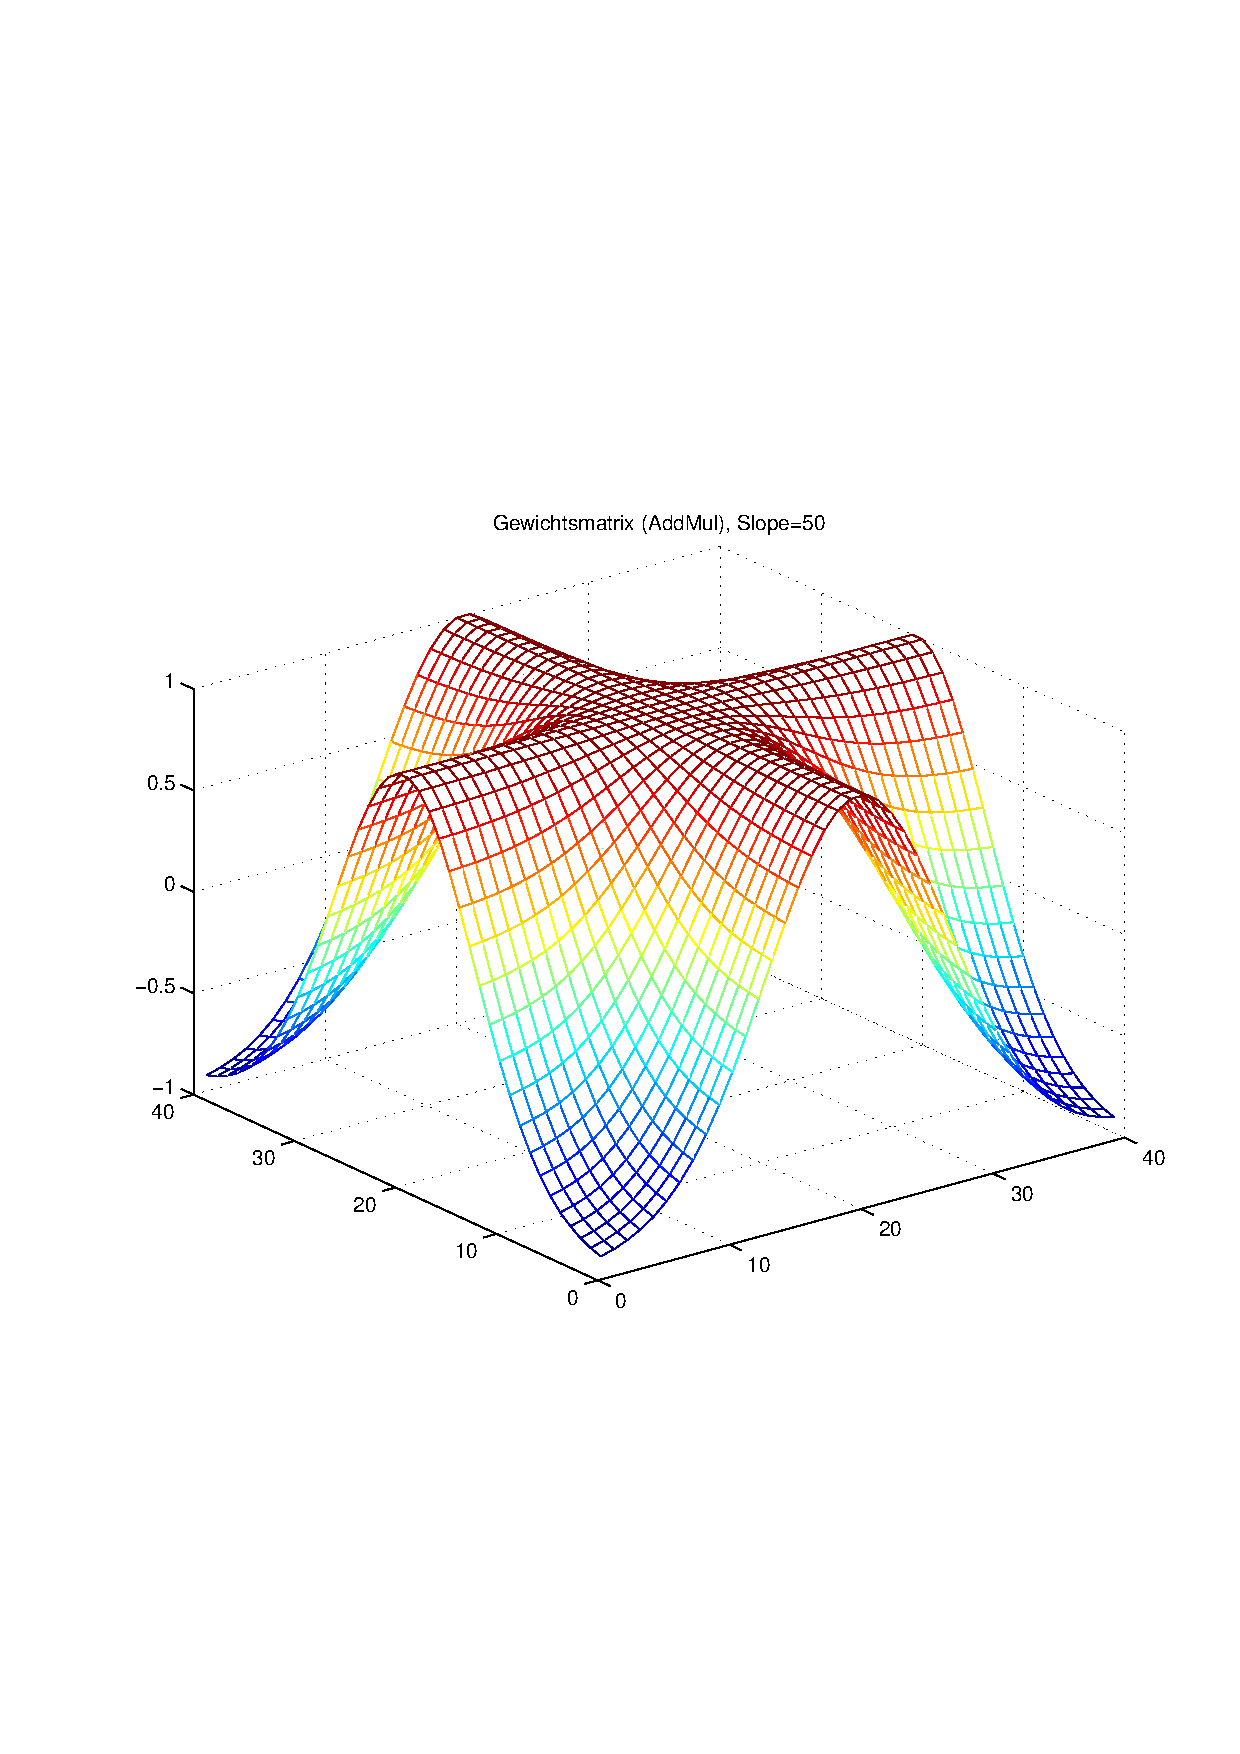
\includegraphics[width=\textwidth]{./Bilder/Auswertung/Gewichtsmatrix/Gewichtsmatrix_AddMul_Slope_50}
		\caption{Additive und Multiplikative Überlagerung mit Slope von 50}
		\label{AddMul50}
	\end{minipage}
\end{figure}

\begin{figure}[hbt]
	\centering
	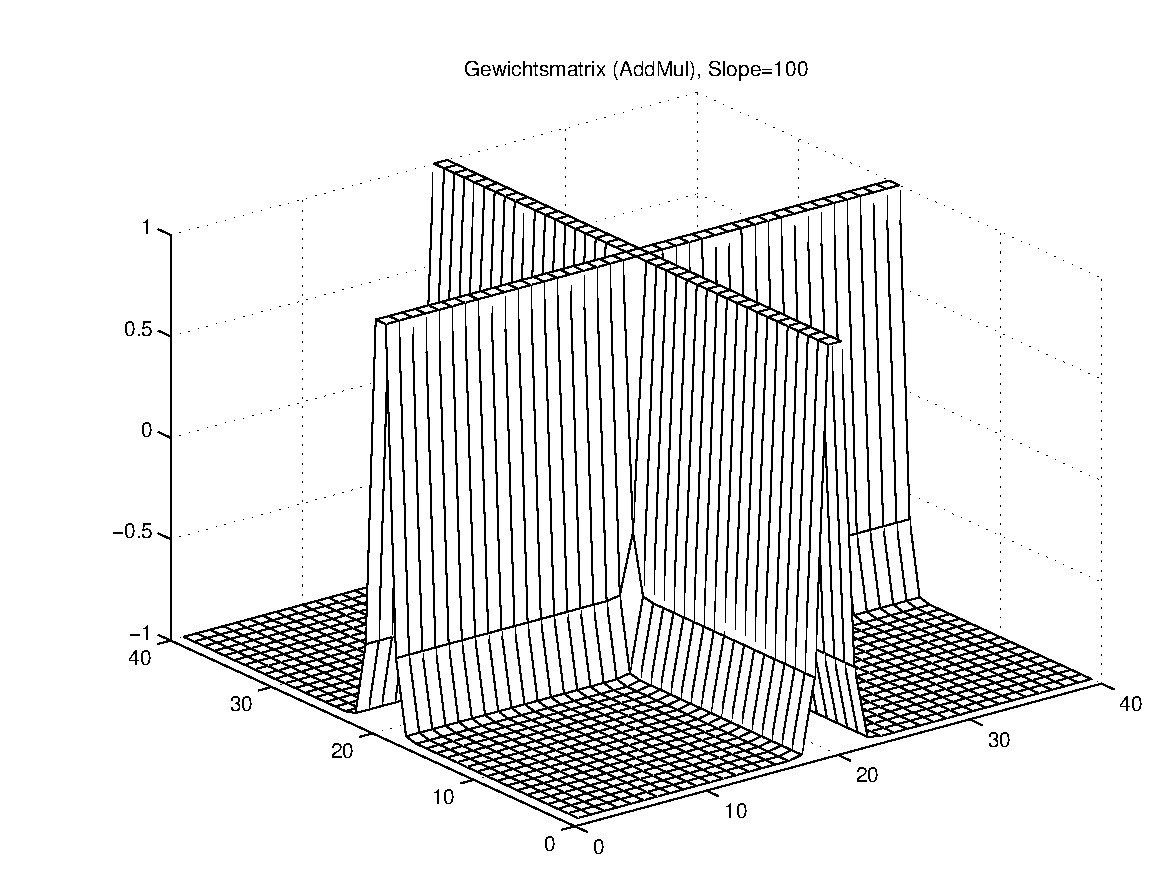
\includegraphics[width=0.6\linewidth]{./Bilder/Auswertung/Gewichtsmatrix/Gewichtsmatrix_AddMul_Slope_100}
	\caption{Additive und Multiplikative Überlagerung mit Slope von 100}
	\label{AddMul100}
\end{figure}

\newpage
\subsection{Spezielle Überlagerung}
\begin{figure}[hbt]
	\begin{minipage}{0.5 \textwidth}
		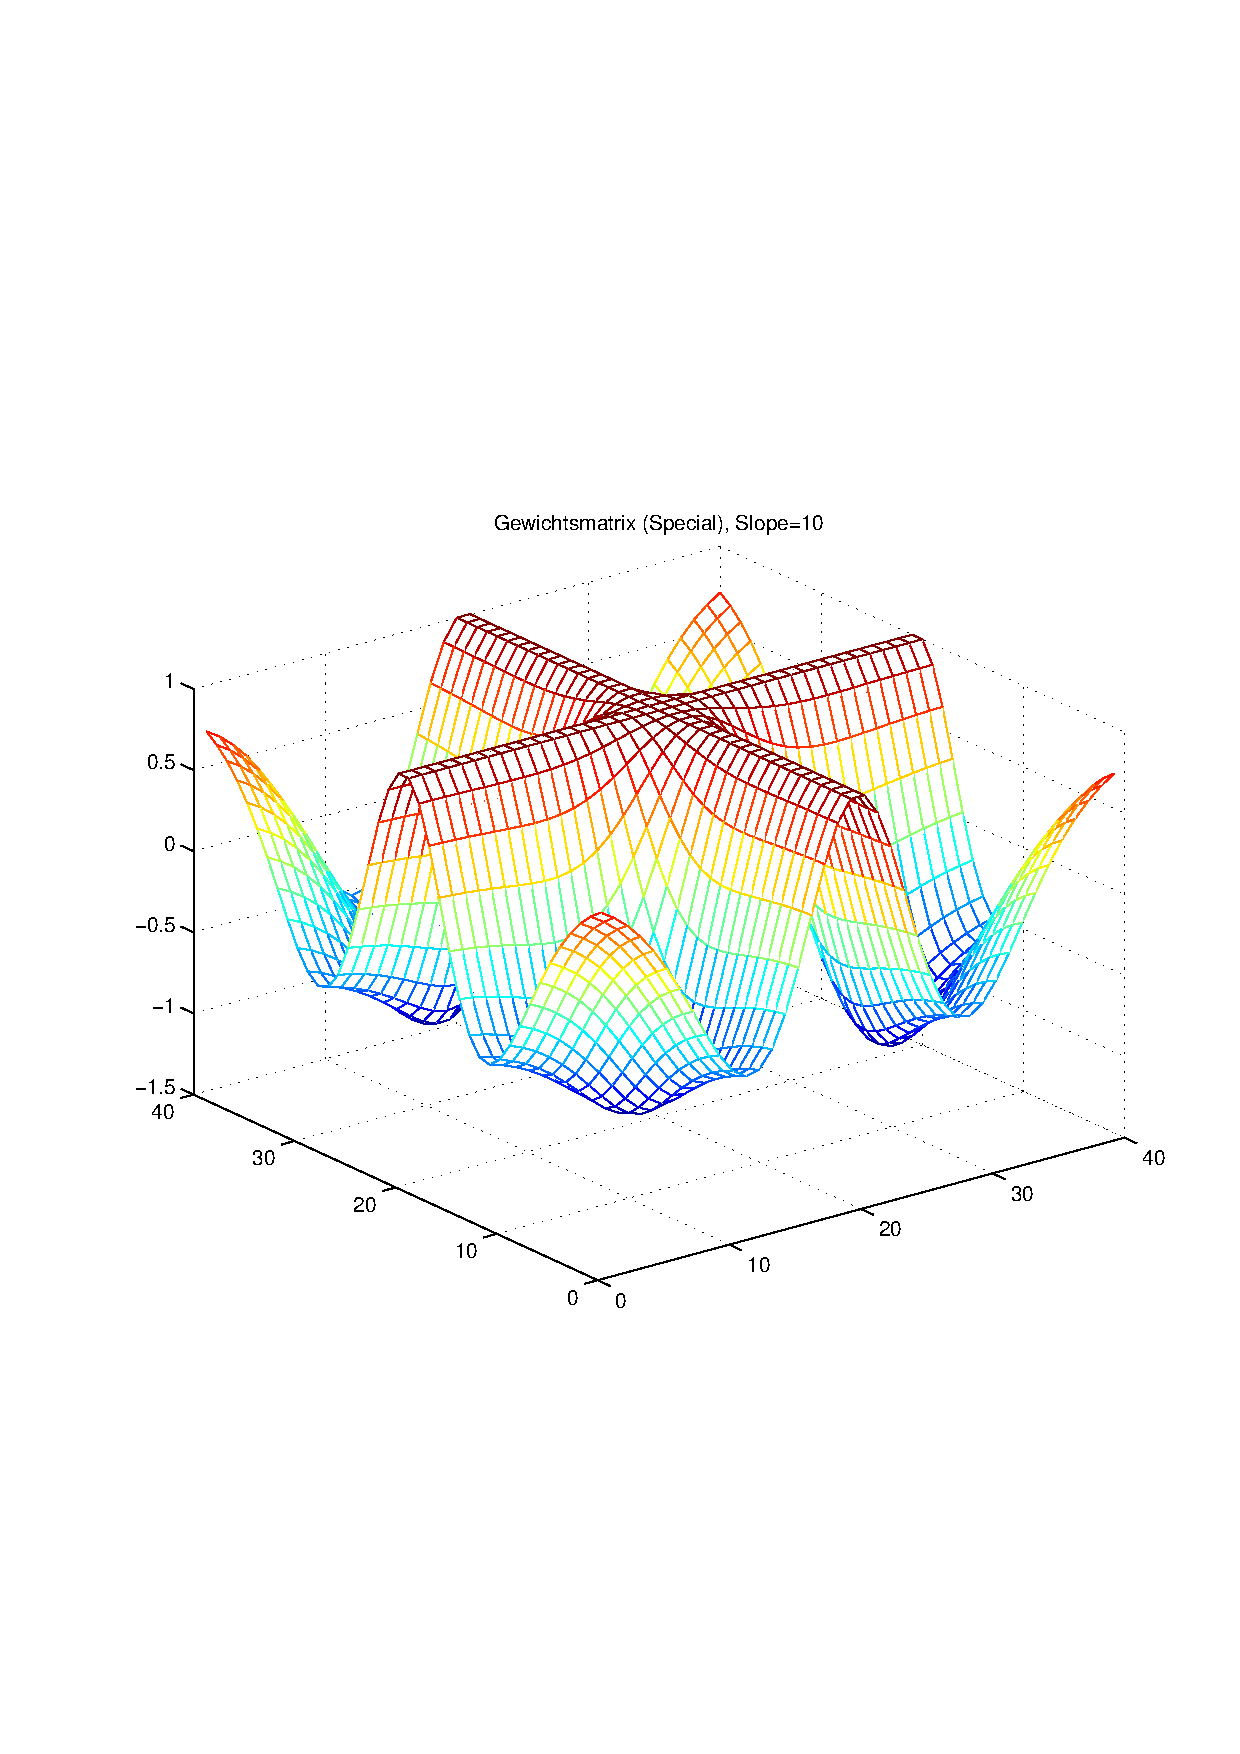
\includegraphics[width=\textwidth]{./Bilder/Auswertung/Gewichtsmatrix/Gewichtsmatrix_Special_Slope_10}
		\caption{Spezielle Überlagerung mit Slope von 10}
		\label{Spez210}
	\end{minipage}
	\hfill
	\begin{minipage}{0.5 \textwidth}
		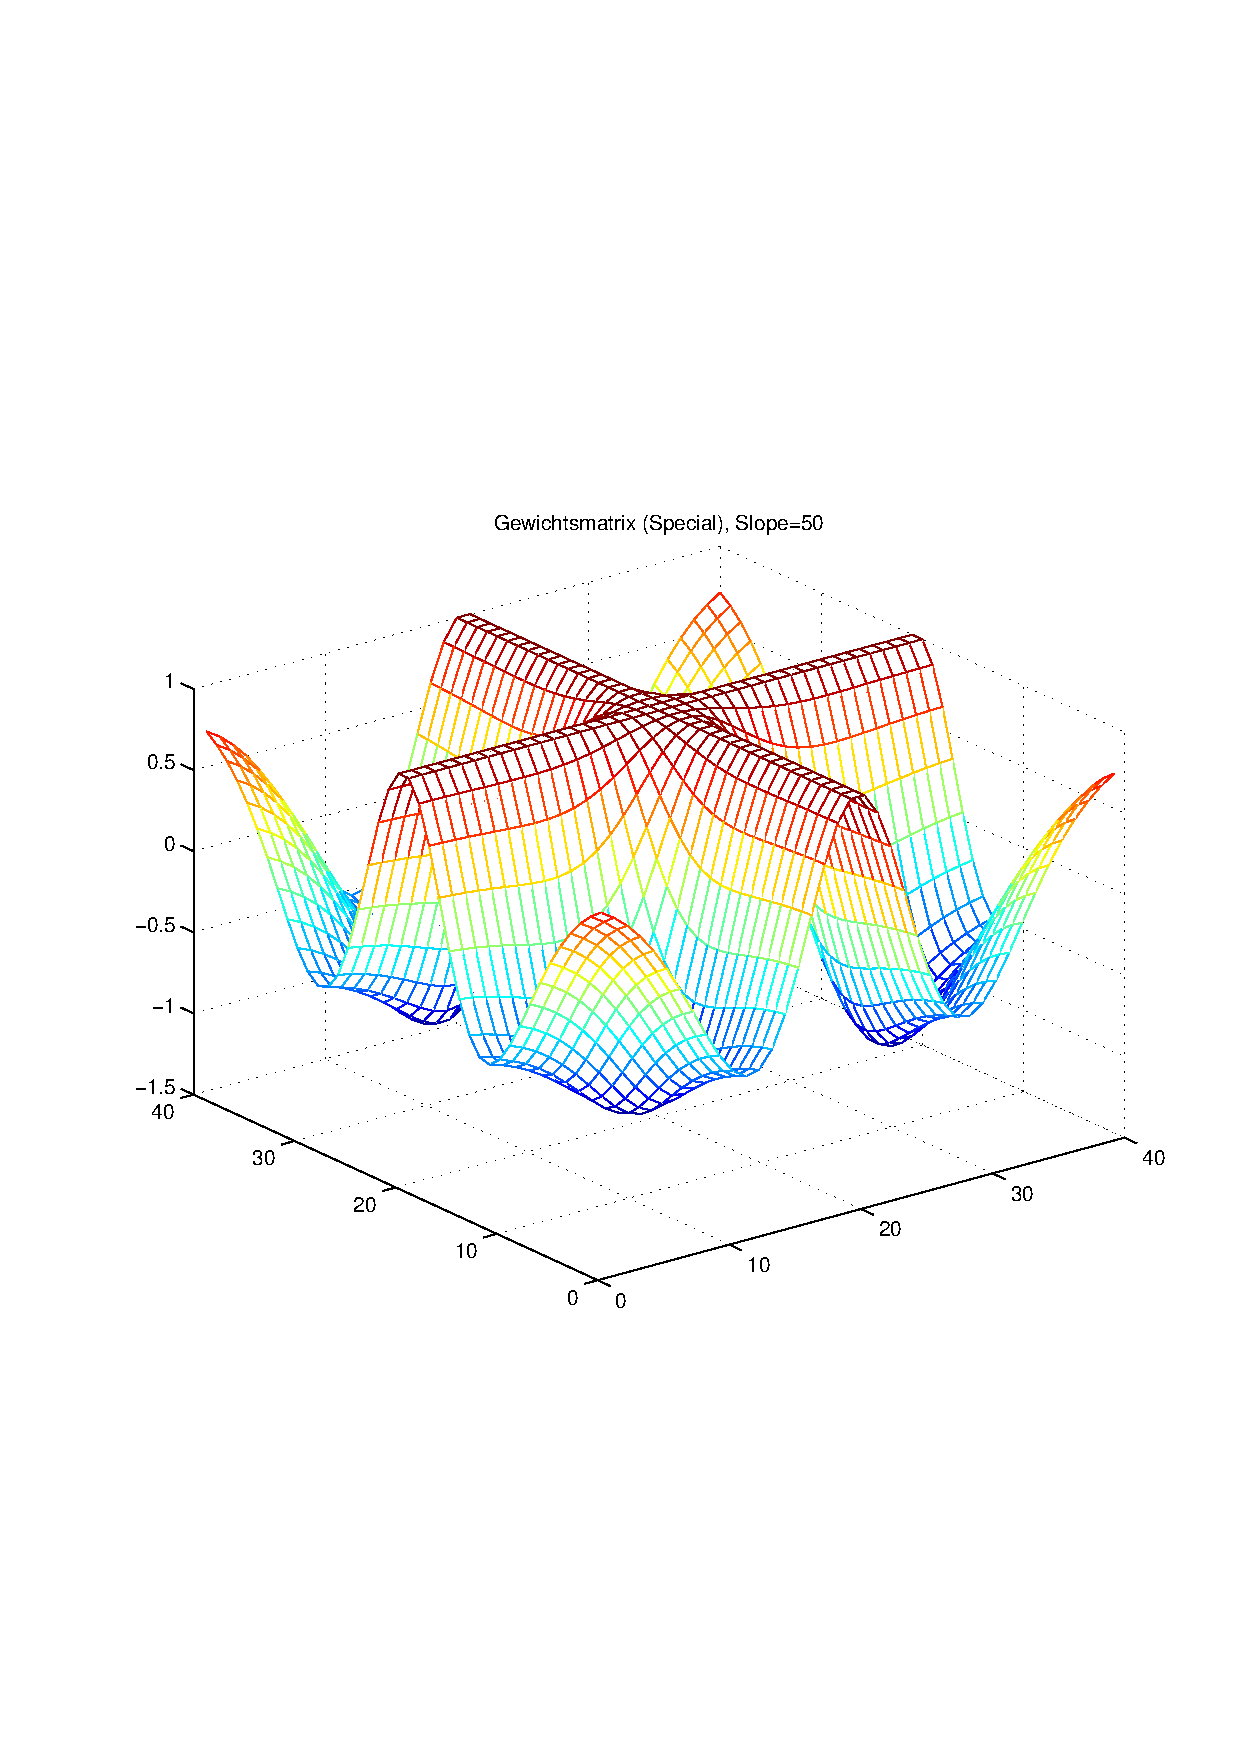
\includegraphics[width=\textwidth]{./Bilder/Auswertung/Gewichtsmatrix/Gewichtsmatrix_Special_Slope_50}
		\caption{Spezielle Überlagerung mit Slope von 50}
		\label{Spezl50}
	\end{minipage}
\end{figure}

\begin{figure}[hbt]
	\centering
	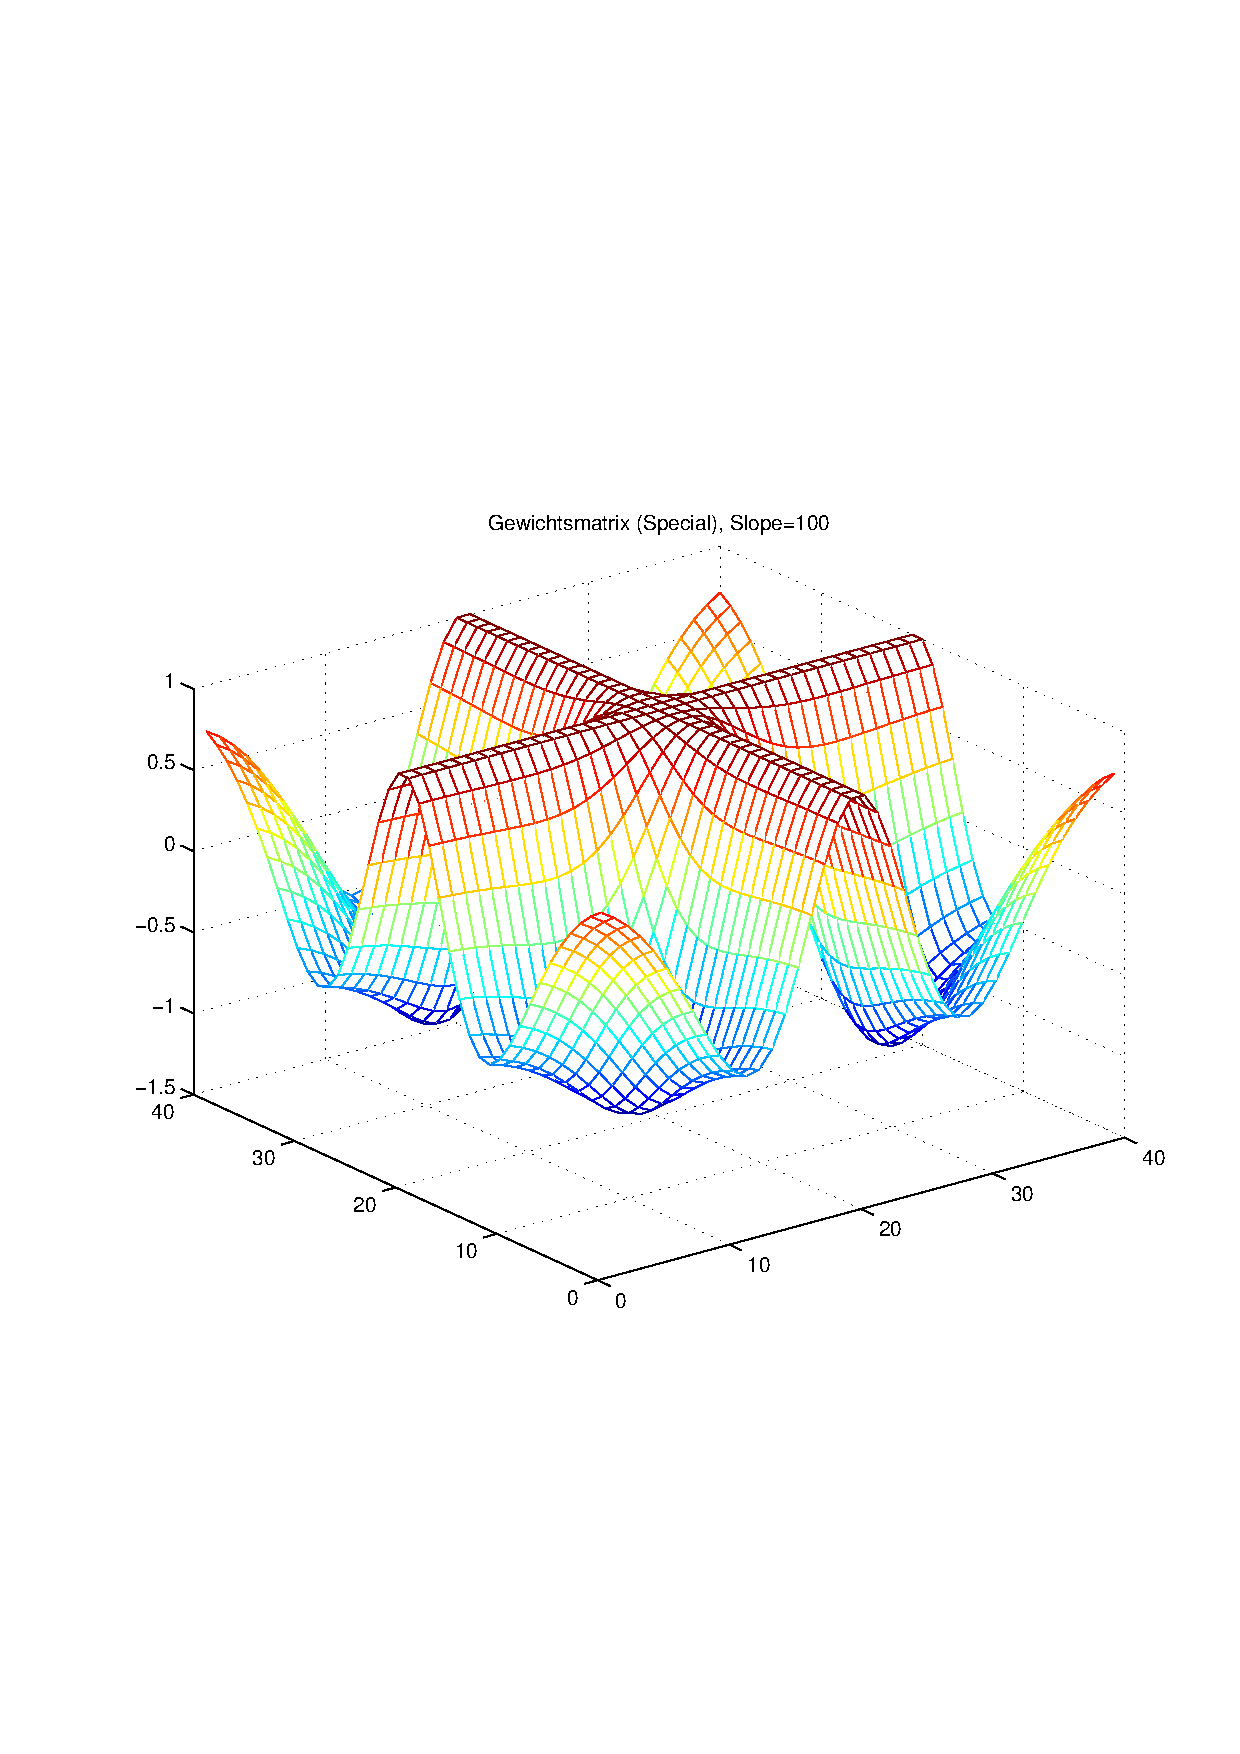
\includegraphics[width=0.6\linewidth]{./Bilder/Auswertung/Gewichtsmatrix/Gewichtsmatrix_Special_Slope_100}
	\caption{Spezielle Überlagerung mit Slope von 100}
	\label{Spez100}
\end{figure}

Bei der Speziellen Gewichtsmatrix hat der Slope keine Auswirkungen. Das war viel mehr ein Versuch, die Auswirkung von erhöhten Gewichten in den Randbereichen zu untersuchen. Aus diesen Grund wurde sie empirisch ermittelt aus den Typen: 'Mul1', 'Mul2' und 'AddMul'.
\newpage
\section{Das Matlab Tool}

Dieser Abschnitt soll dazu dienen, die Matlab-Skripte besser verstehen zu können. Es soll keine komplette Anleitung sein, aber die wichtigsten Zusammenhänge darstellen und Erfahrungswerte darlegen. In diesem Projekt sind viele Zeile Code in Matlab geschrieben worden. Es sollte erreicht werden, dass der Aufbau der einzelnen Dateien möglichst generisch ist. Die Entwicklung hat mithilfe von GitHub stattgefunden. Darüber können auch die Skripte und Dokumentation heruntergeladen werden.


\subsection{Modulübersicht}
Die Matlab-Skripte können in Kategorien eingeteilt werden. Die folgende Übersicht soll darüber Aufschluss geben. 

\begin{itemize}
	\item Ablauf und Einstellungen:
	
	In diesen Dateien werden alle benötigten Module aufgerufen. In 'main.m' ist der komplette Ablauf hinterlegt. Für eine bessere Reproduzierbarkeit haben wir zwei weitere Dateien angelegt, in denen wir Grundeinstellungen getroffen haben für Gewichtsmatrizen, die wir in der Dokumentation auswerten.
	
	\begin{itemize}
		\item main.m
		\item SettingFileAddMul.m
		Einstellungen für die Gewichts-Matrix 'AddMul'.
		
		\item SettingFileSpecial.m
		Einstellungen für die Gewichts-Matrix 'Special'.
		
	\end{itemize}
	
	\item Module:
	
	In dieser Auflistung werden alle relevanten Module gezeigt, welche für die Grundfunktionen verantwortlich sind.
	
	\begin{itemize}
		\item GetPixelFeatureMatrix.m
		Diesem Modul wird eine Merkmale-Matrix übergeben und das Modul skaliert dann die Merkmale-Matrix auf eine Pixel-Matrix. Außerdem kann dem Modul ein Rauschwert zwischen 0\% und 100\% übergeben werden, um die Bilder mit Rauschen zu versehen. Das Modul gibt die Pixel-Matrix zurück und kann die erzeugten Bilder auch gleich als Datei speichern.
		
		\item GetNeuronOutput.m
		Dieses Modul ist das eigentliche Neuron. Es müssen als Parameter die Eingangszustände und Gewichte übergeben werden. Es berechnet anschließend über die Aktivierungsfunktion das Ergebnis. Es werden darüber hinaus auch Zwischenergebnisse zurückgegeben.
		
		\item GetInputFeatureMatrix.m
		Dieses Modul gibt vordefinierte Merkmale-Matrizen zurück, die wir häufig verwendet haben.
		
		\item GetGaussWeights.m
		Dieses Modul gibt eine Gewichts-Matrix zurück. Welche hinterlegt sind kann im Abschnitt \ref{gewichtsmatrizenSection} nachgeschaut werden.
		
		\item GetFeatureOfMatrix.m
		Diesem Modul kann eine Pixel-Matrix übergeben werden und gibt eine Merkmale-Matrix zurück.
		
		\item ConvMatrixToColumn.m
		Das Modul konvertiert eine Merkmale-Matrix in einen Spaltenvektor.
		
	\end{itemize}
	
	\item Funktionen:
	
	Diese Funktionen wurden von uns implementiert. Im akutellen Stand wurde allerdings nur die Gauß- und Sigmoid-Funktion verwendet.
	
	\begin{itemize}
		\item GaussNormFunction.m
		\item SigmoidFunction.m
		\item LinearFunction.m
		\item RayleighFunction.m
		\item TangHFunction.m
	\end{itemize}

	\item Hilfsfunktionen:
	
	Die Hilfsfunktionen haben für das eigentliche Tool keine oder kaum Bedeutung. Sie werden nur genutzt, um Module zu testen oder Ausgaben zu generieren.
	
	\begin{itemize}
		\item TestTangHFunction.m
		\item TestSigmoidFunction.m
		\item TestRayleighFunction.m
		\item TestLinearFunction.m
		\item TestGetPixelFeatureMatrix.m
		\item TestGetGaussWeights.m
		\item TestGetFeatureOfMatrix.m
		\item TestGaussNormFunction.m
		\item SummaryWeights.m
		\item SummaryFunctions.m
		\item savePic.m
	\end{itemize}
	
\end{itemize}

\subsection{Erläuterung der Parameter}
In dem Matlab-Skript 'main.n' und die abgeleiteten Skripte 'SettingFileAddMul' und 'SettingFileSpecial' sind viele Parameter enthalten, die eingestellt werden können. Dieser Abschnitt soll einen Überblick geben, was die einzelnen Parameter bewirken.

\begin{table}[hbt]
	\centering
	\begin{tabular}{|c|c|c|}
		
		\hline 
		Zeile & Parameter & Erläuterung \\ 
		\hline 
		5 & pixelCnt & Pixel Anzahl in x- und y-Richtung \\ 
		\hline 
		6 & featureCnt & Merkmal Anzahl in x- und y-Richtung \\ 
		\hline 
		7 & weightType & Typ der Gewichts-Matrix (AddMul, Special, Add, Mul1, Mul2) \\ 
		\hline 
		8 & inFeatureType & voreingestellten Merkmale-Matrizen (Cross, H\_Line, V\_Line) \\ 
		\hline 
		9 & noise & Verrauschungsgrad zwischen 0\% und 100\% \\ 
		\hline 
		10 & slope & Steigung der Aktivierungs-Funktion \\ 
		\hline 
		13 & bias & Verschiebung der Aktivierungsfunktion (negativ nach rechts) \\ 
		\hline 
		14 & threshold & Auswertungsschwelle des Ergebnisses \\ 
		\hline 
		15 & domainOfDefinition & Gueltigkeitsbereich der Neuronenfunktion (+/-) \\ 
		\hline 
		18 & lowerBound & Untere Grenze der Gewichts-Matrix \\ 
		\hline 
		19 & upperBound & Obere Grenze der Gewichts-Matrix \\ 
		\hline 
		125 & domainOfDefinition & 2. Neuronen Ebene, h-Balken \\ 
		\hline
		126 & bias & 2. Neuronen Ebene, h-Balken \\ 
		\hline 
		127 & threshold & 2. Neuronen Ebene, h-Balken \\ 
		\hline 
		151 & domainOfDefinition & 2. Neuronen Ebene, v-Balken \\ 
		\hline
		152 & bias & 2. Neuronen Ebene, v-Balken \\ 
		\hline 
		153 & threshold & 2. Neuronen Ebene, v-Balken \\ 
		\hline 
		177 & domainOfDefinition & 2. Neuronen Ebene, Fehler Detektion \\ 
		\hline
		178 & bias & 2. Neuronen Ebene, Fehler Detektion \\ 
		\hline 
		179 & threshold & 2. Neuronen Ebene, Fehler Detektion \\ 
		\hline 
		
	\end{tabular}
	\caption{Übersicht der Parameter}
	
	\label{ueParameter}
\end{table}

\newpage
\section{Auswertung}
Für die Auswertung haben wir haben zwei von den vorgestellten Gewichtsmatrizen untersucht. Wir haben uns für die Gewichtsmatrizen 'AddMul' und 'Special' entschieden. Um reproduzierbare Ergebnisse liefern zu können, haben wir aus der 'main.m' zwei Dateien abgeleitet in denen die Konfigurationen der nachfolgenden Bilder hinterlegt sind. Die beiden Dateien heißen 'SettingFileAddMul.m' und 'SettingFileSpecial.m'. Beide Systeme wurde empirisch eingestellt und es wurde versucht ab einem Rauschen von 50\% keine vernünftigen Ergebnisse mehr zu liefern. Außerdem wurden die Bias-Werte und Threshold-Werte voreingestellt.

Als nächstes soll für ein Beispiel besprochen werden, wie die Grafiken zu lesen sind. Dafür benutzen wir die Abbildungen \ref{AddMul_H_40_1} und \ref{AddMul_H_40_2} heran. Untersucht wurde die AddMul-Gewichtsmatrix mit horizontalen Balken. Der Rauschwert ist auf 40\% eingestellt. Die Farbe der eingezeichneten Punkte gibt an, ob das jeweilige Merkmal richtig detektiert wurde oder nicht. In Abbildung \ref{AddMul_H_40_1} sehen wir das Ergebnis der ersten Neuronen Ebene. In der Sigmoid-Grafik sind 25 grüne Punkte eingezeichnet. Es sind also alle Merkmale richtig detektiert worden. An dieser Stelle werden die addierten Werte der einzelnen Pixel auf eine Sigmoid-Funktion gegeben und grafisch ausgewertet.

In Abbildung \ref{AddMul_H_40_2} ist die zweite Neuronen-Ebene dargestellt. In jeder Grafik ist jeweils ein Punkt eingezeichnet. In der Grafik der 'h-Balken Detektion' ist ein grüner Punkt eingezeichnet, d.h. es wurde ein 'h-Balken' detektiert. In der Grafik der 'v-Balken Detektion' ist ein roter Punkt eingezeichnet, d.h. es wurde kein 'v-Balken' detektiert. Die letzte Grafik der zweiten Neuronen Ebene ist die 'Fehler Detektion'. In diesem Fall ist der Punkt grün, also wurde keinen Fehler detektiert. Die 'Fehler Detektion' soll angeben, wenn der voreingestellte Rauschwert überschritten wurde. Es ist zu beachten, dass die Werte aus der ersten Ebene nicht mit der Sigmoid-Funktion bearbeitet wurden, sondern lediglich mit einer linearen Aktivierungsfunktion mit dem Anstieg 1, d.h. die addierten Werte der Pixel pro Merkmal werden direkt weitergereicht.  

\newpage
\subsection{AddMul Gewichtsmatrix}
\subsubsection{H-Balken}
\begin{figure}[hbt]
	\centering
	\begin{minipage}[c]{\textwidth}
       	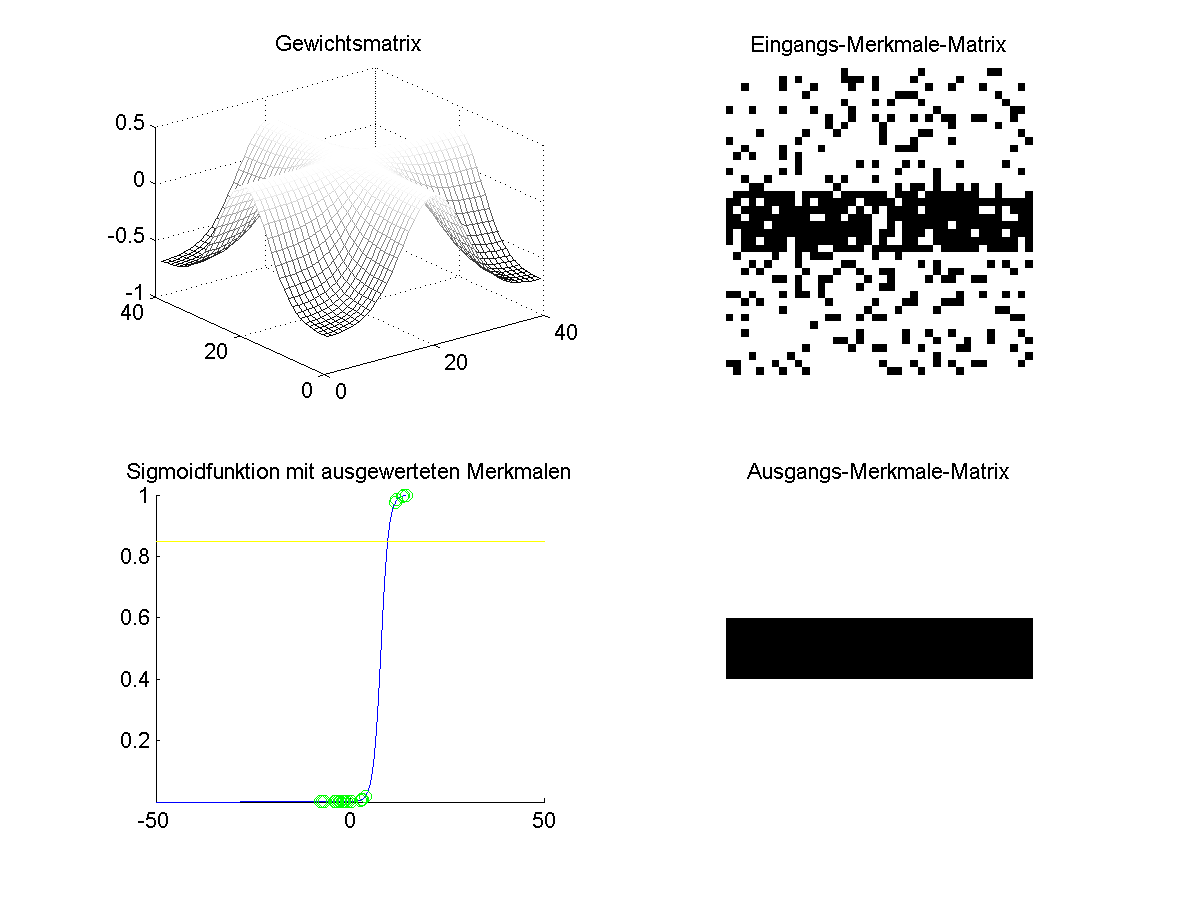
\includegraphics[trim=70 211 42 222, clip, width=0.9\textwidth]{./Bilder/Auswertung/Endergebnis/TypeAddMul_Rauschen40_H_Line_Layer1}
		\caption{AddMul, H-Balken, 40\% Rauschen, 1. Neuronen Ebene}
		\label{AddMul_H_40_1}
		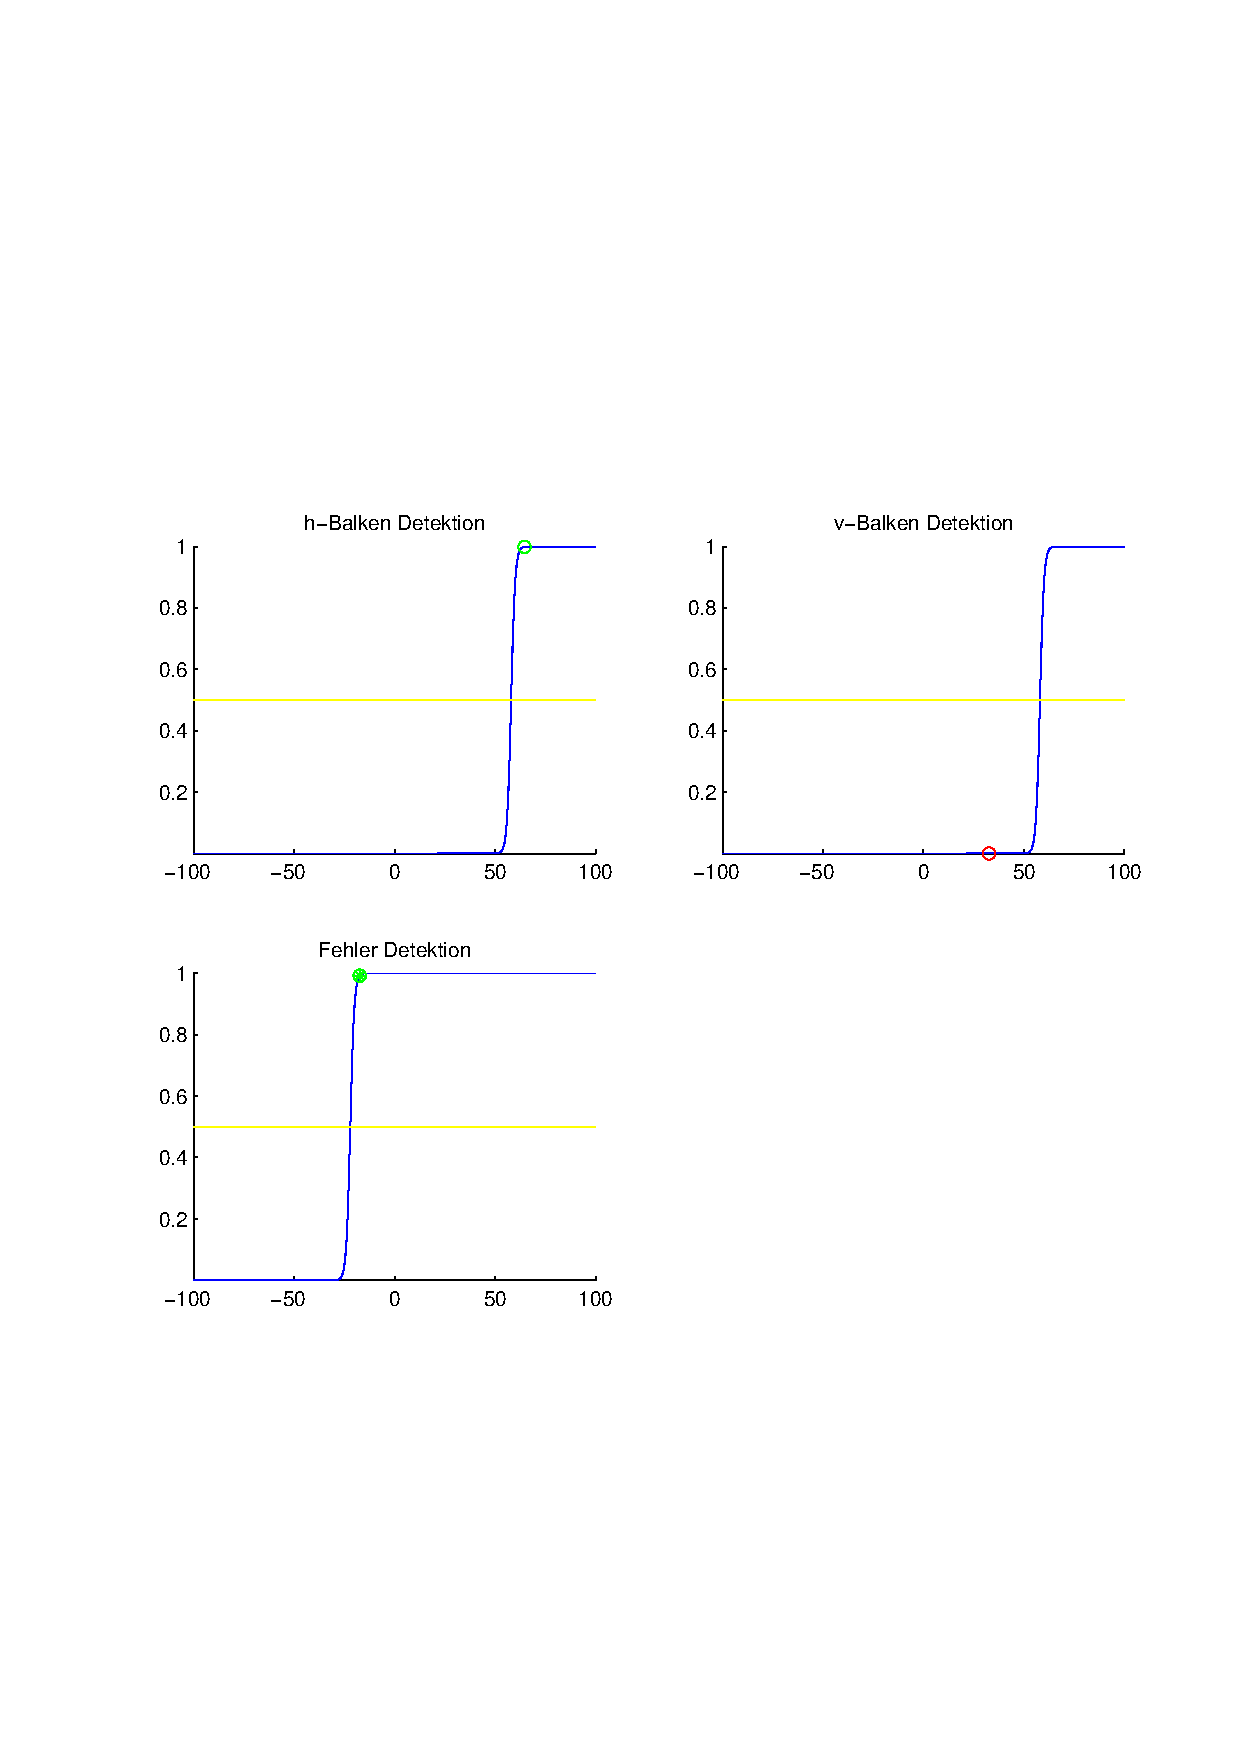
\includegraphics[trim=70 211 42 222, clip, width=0.9\textwidth]{./Bilder/Auswertung/Endergebnis/TypeAddMul_Rauschen40_H_Line_Layer2}
		\caption{AddMul, H-Balken, 40\% Rauschen, 2. Neuronen Ebene}
		\label{AddMul_H_40_2}
	\end{minipage}
\end{figure}

\begin{figure}[hbt]
	\begin{minipage}{0.8 \textwidth}
		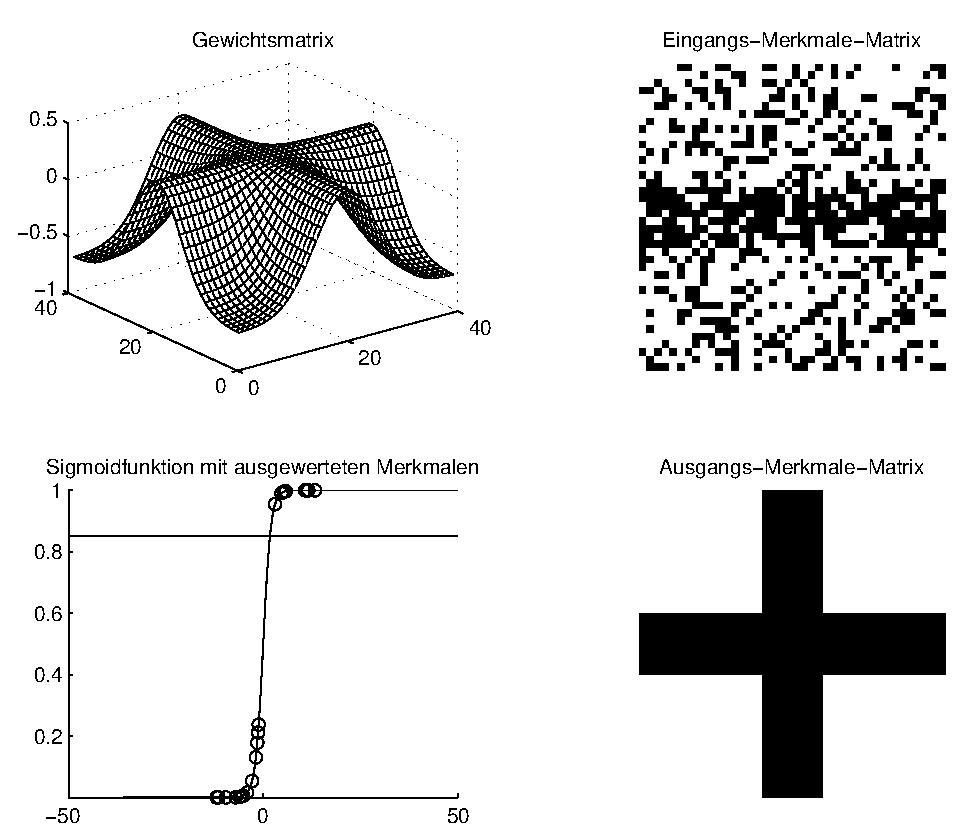
\includegraphics[width=\textwidth]{./Bilder/Auswertung/Endergebnis/TypeAddMul_Rauschen60_H_Line_Layer1}
		\caption{AddMul, H-Balken, 60\% Rauschen, 1. Neuronen Ebene}
		\label{AddMul_H_60_1}
	\end{minipage}
	\vfill
	\begin{minipage}{0.8 \textwidth}
		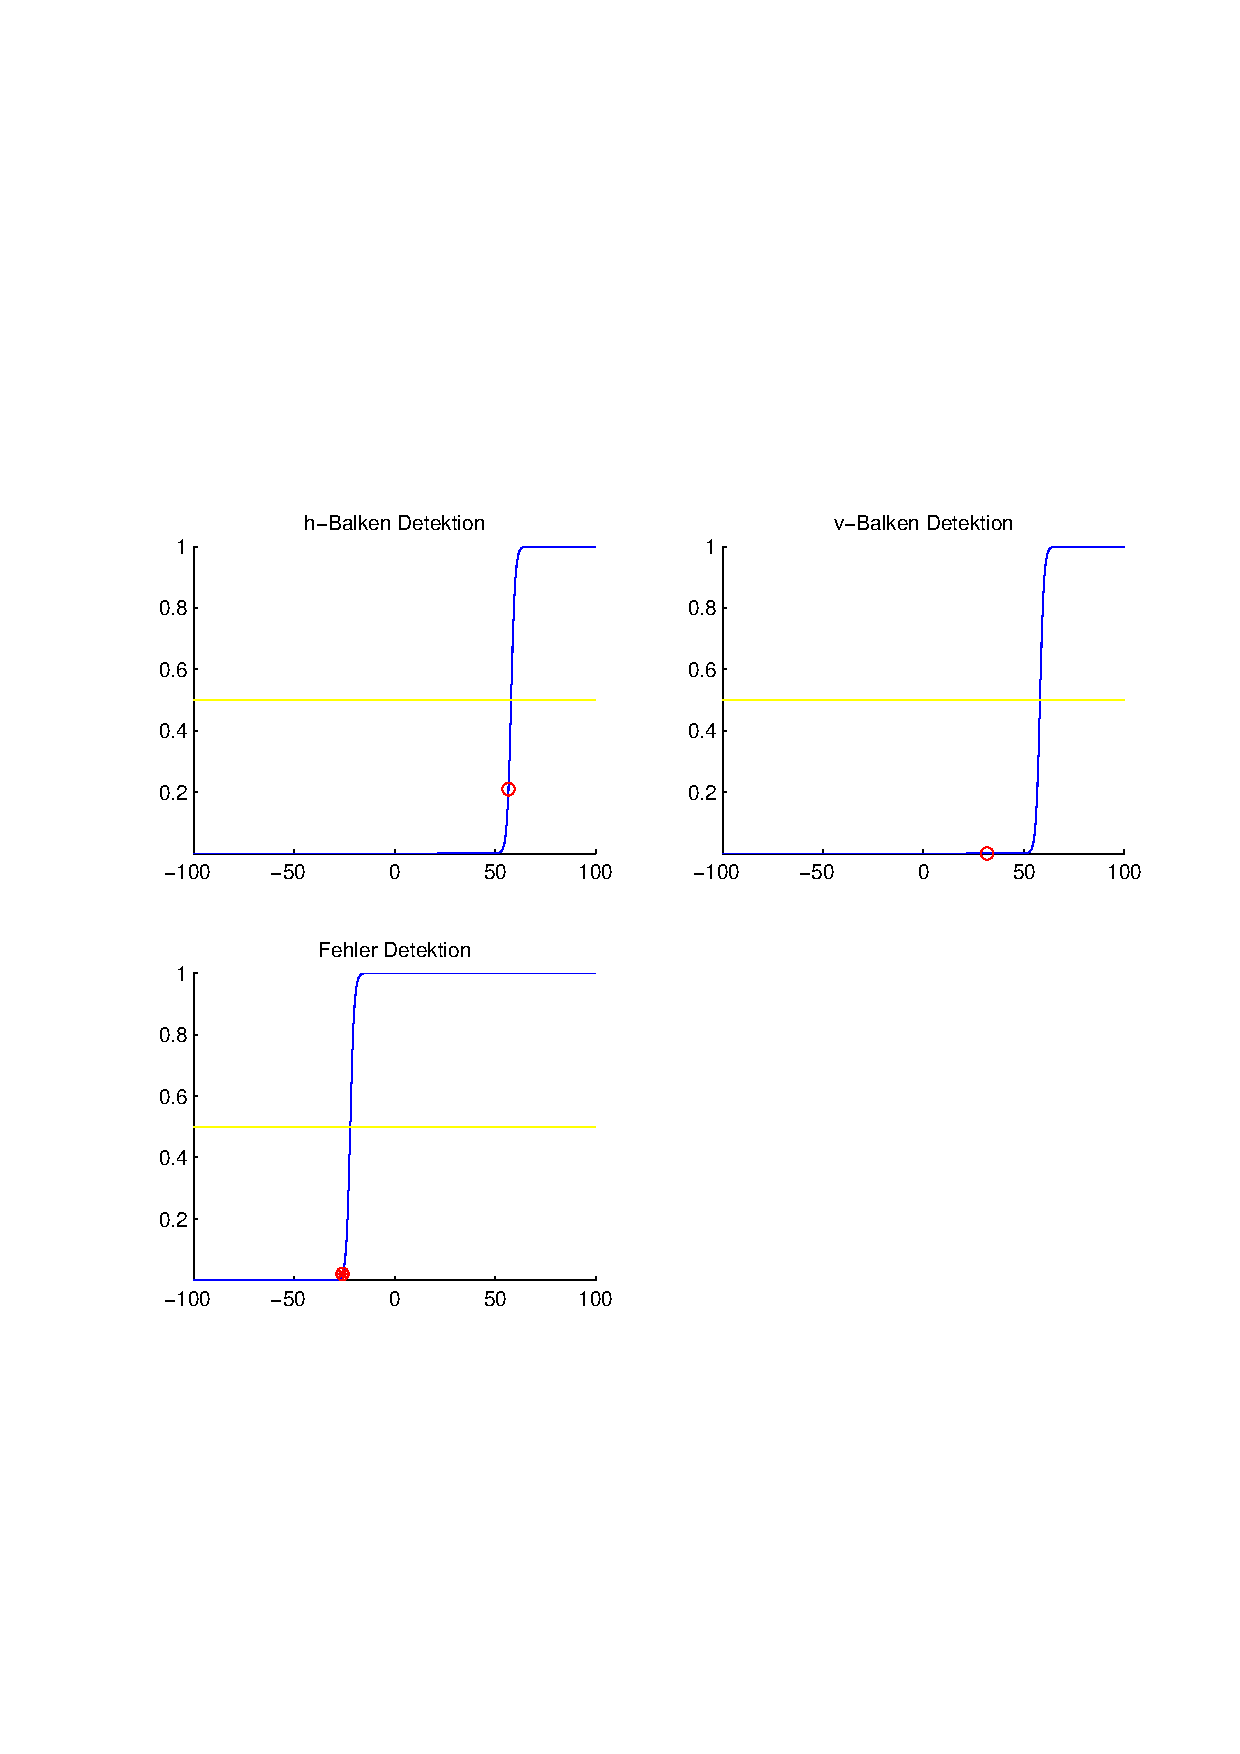
\includegraphics[width=\textwidth]{./Bilder/Auswertung/Endergebnis/TypeAddMul_Rauschen60_H_Line_Layer2}
		\caption{AddMul, H-Balken, 60\% Rauschen, 2. Neuronen Ebene}
		\label{AddMul_H_60_2}
	\end{minipage}
\end{figure}

\begin{figure}[hbt]
	\begin{minipage}{0.8 \textwidth}
		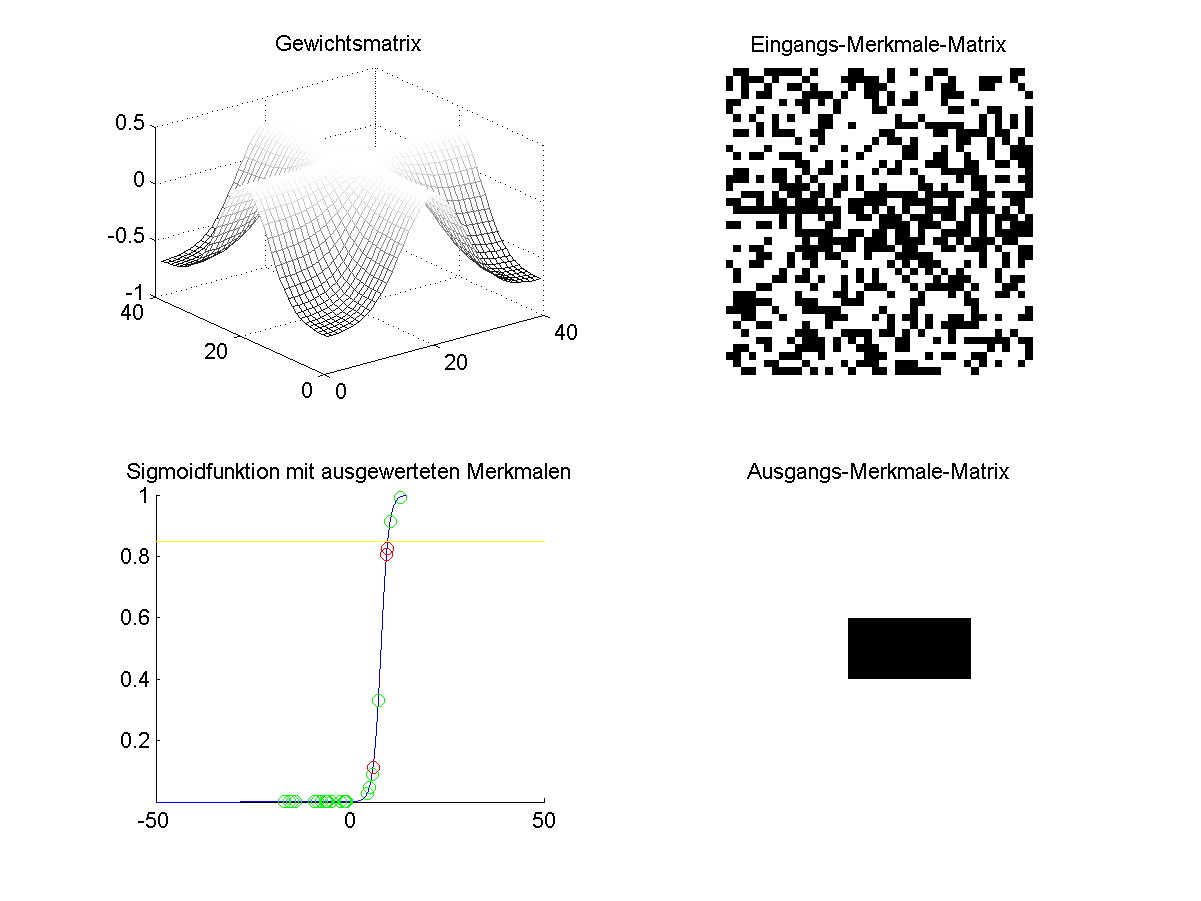
\includegraphics[width=\textwidth]{./Bilder/Auswertung/Endergebnis/TypeAddMul_Rauschen80_H_Line_Layer1}
		\caption{AddMul, H-Balken, 80\% Rauschen, 1. Neuronen Ebene}
		\label{AddMul_H_80_1}
	\end{minipage}
	\vfill
	\begin{minipage}{0.8 \textwidth}
		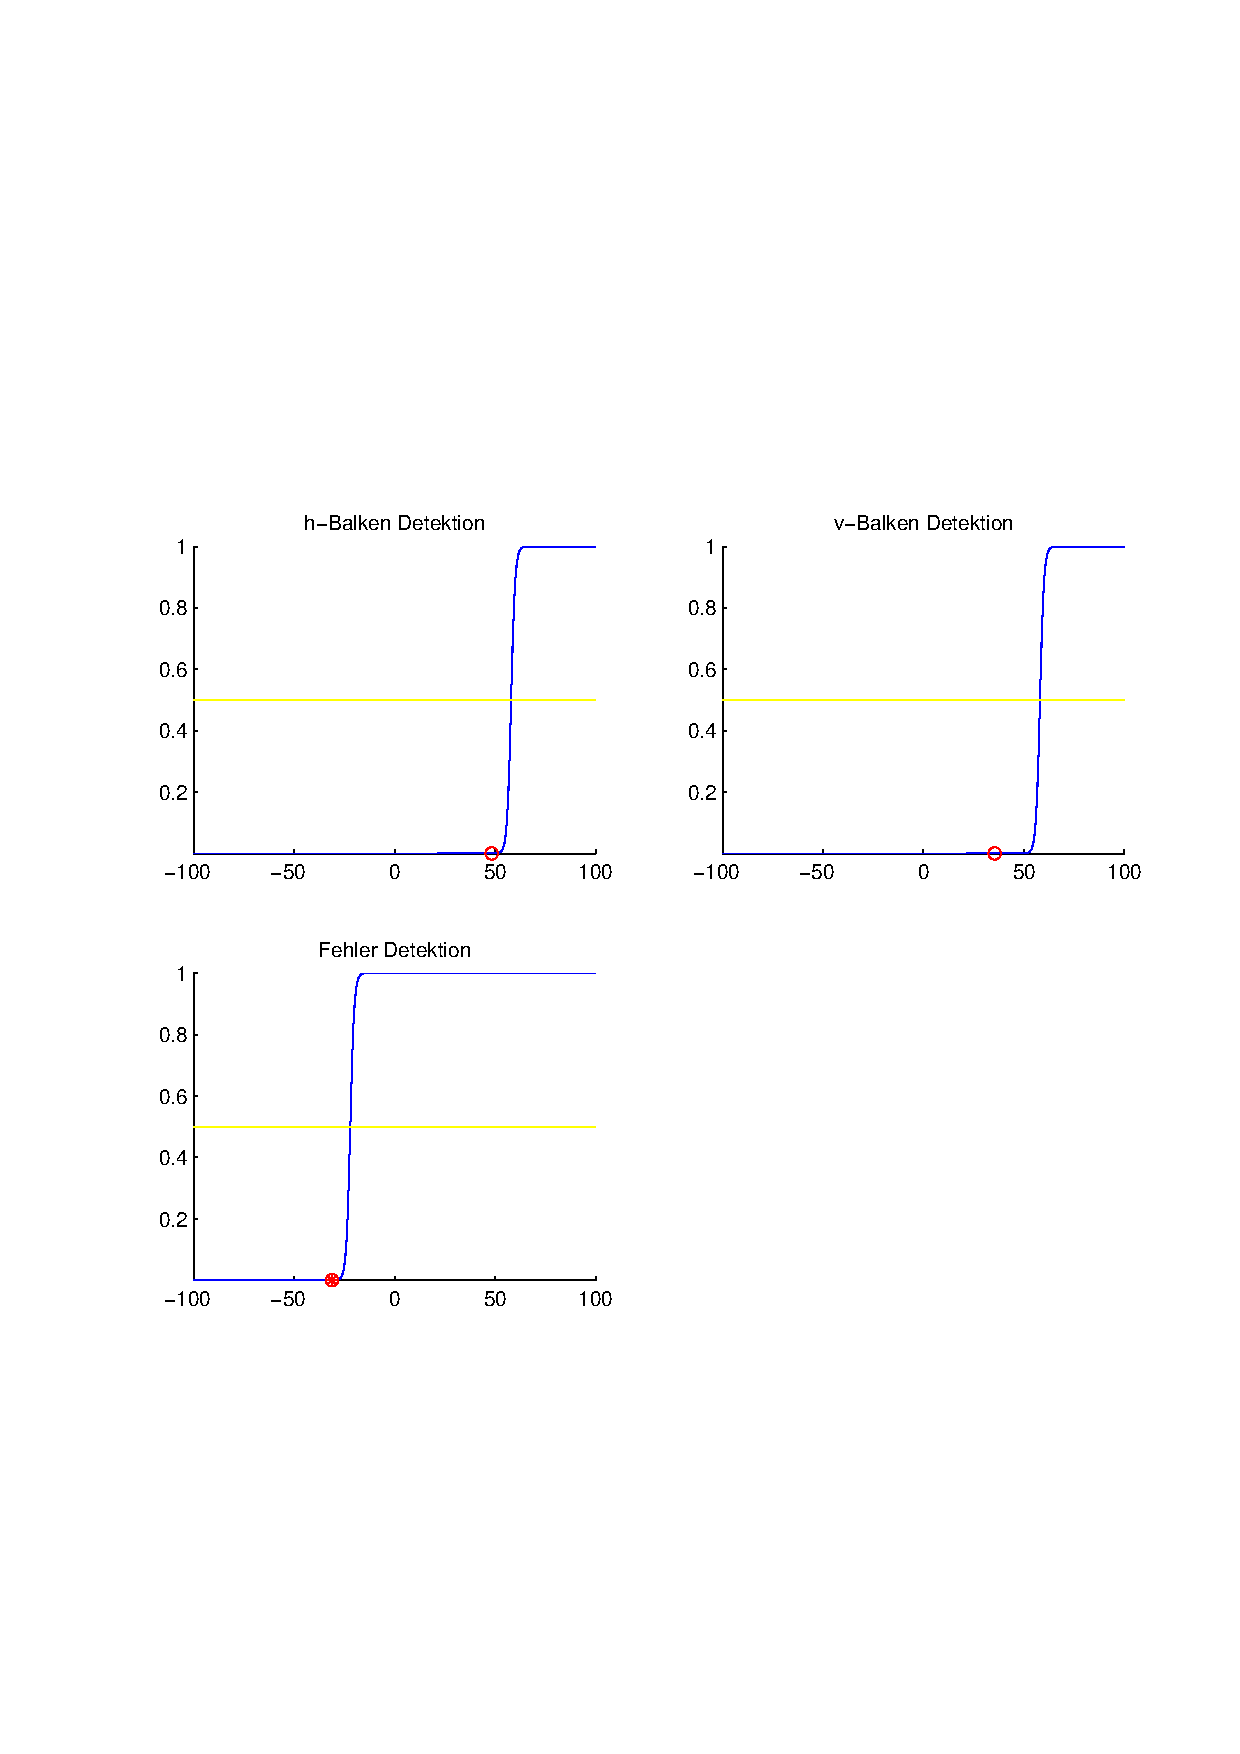
\includegraphics[width=\textwidth]{./Bilder/Auswertung/Endergebnis/TypeAddMul_Rauschen80_H_Line_Layer2}
		\caption{AddMul, H-Balken, 80\% Rauschen, 2. Neuronen Ebene}
		\label{AddMul_H_80_2}
	\end{minipage}
\end{figure}
\clearpage

\subsubsection{V-Balken}
\begin{figure}[hbt]
	\begin{minipage}{0.8 \textwidth}
		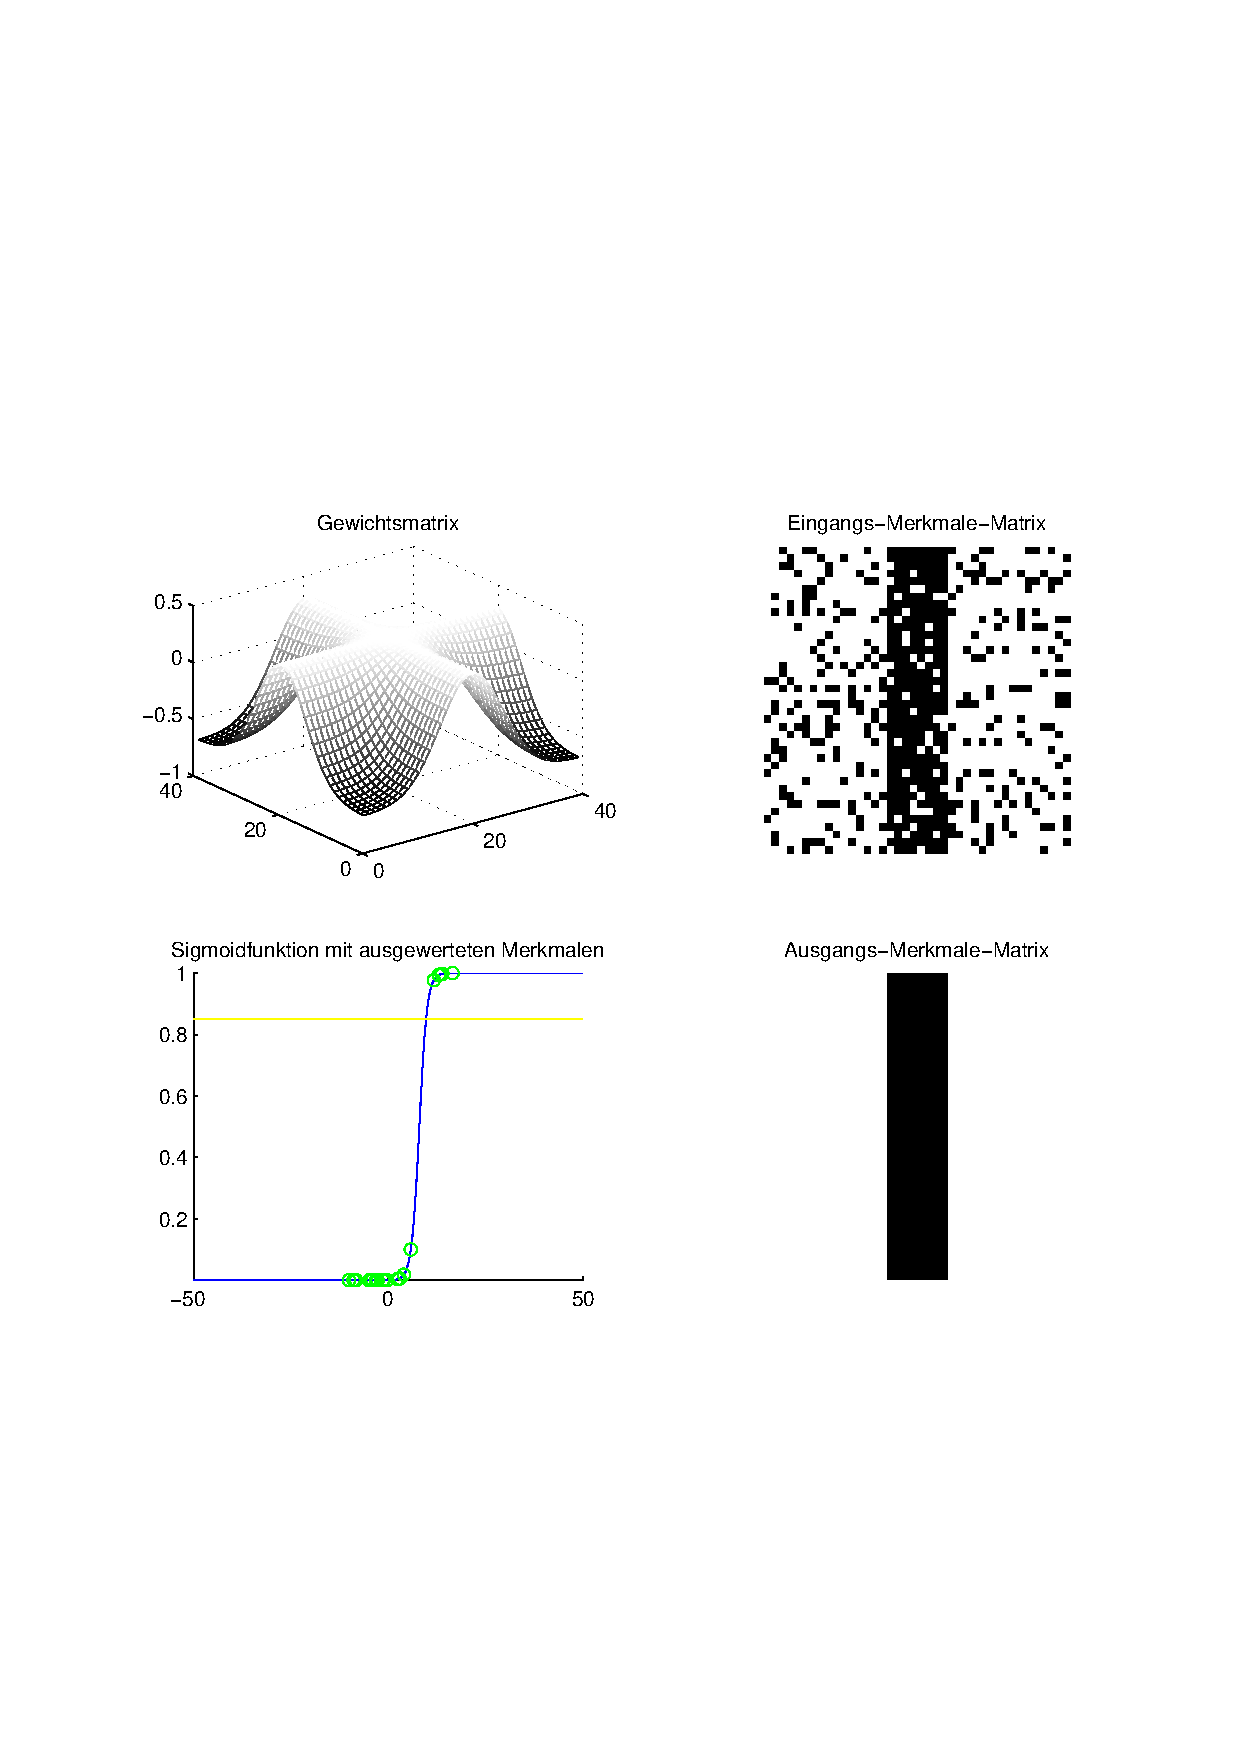
\includegraphics[width=\textwidth]{./Bilder/Auswertung/Endergebnis/TypeAddMul_Rauschen40_V_Line_Layer1}
		\caption{AddMul, V-Balken, 40\% Rauschen, 1. Neuronen Ebene}
		\label{AddMul_V_40_1}
	\end{minipage}
	\vfill
	\begin{minipage}{0.8 \textwidth}
		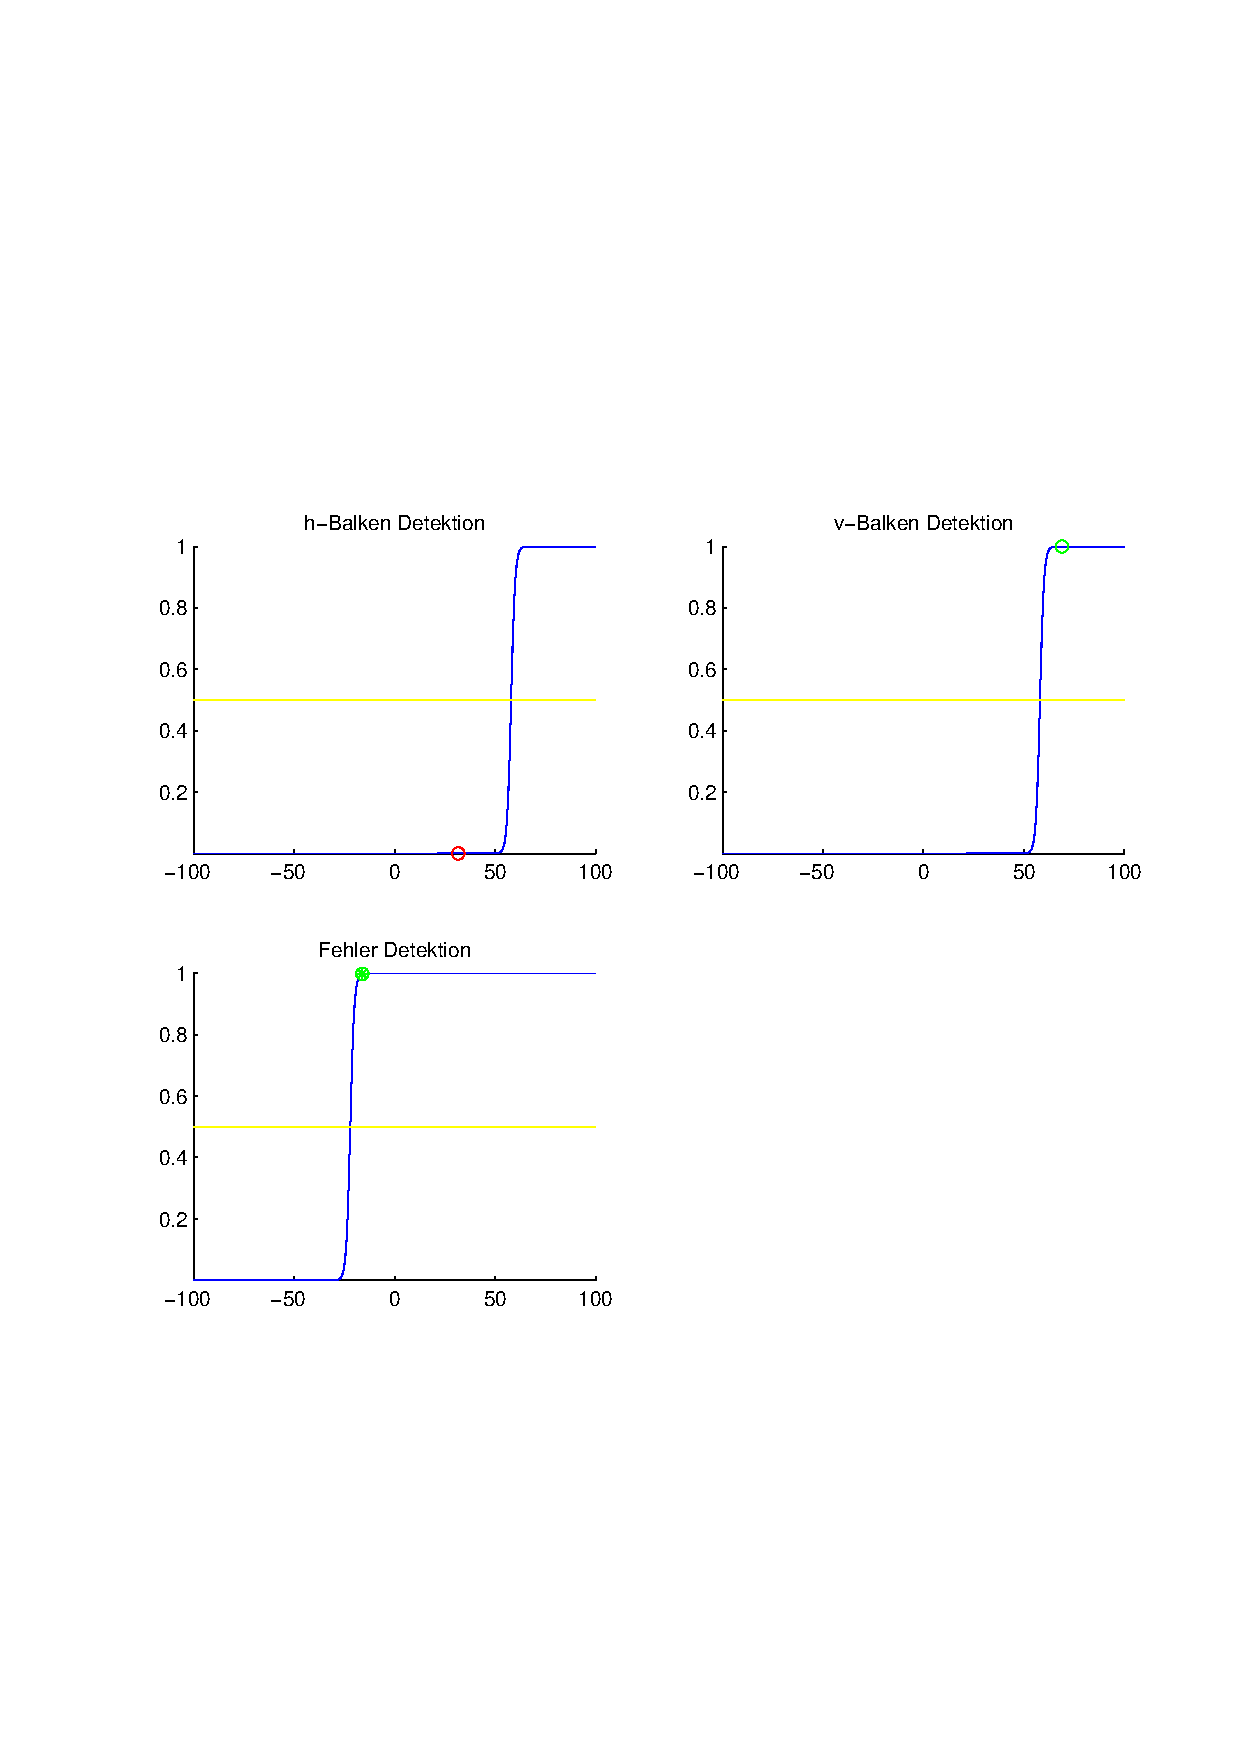
\includegraphics[width=\textwidth]{./Bilder/Auswertung/Endergebnis/TypeAddMul_Rauschen40_V_Line_Layer2}
		\caption{AddMul, V-Balken, 40\% Rauschen, 2. Neuronen Ebene}
		\label{AddMul_V_40_2}
	\end{minipage}
\end{figure}

\begin{figure}[hbt]
	\begin{minipage}{0.8 \textwidth}
		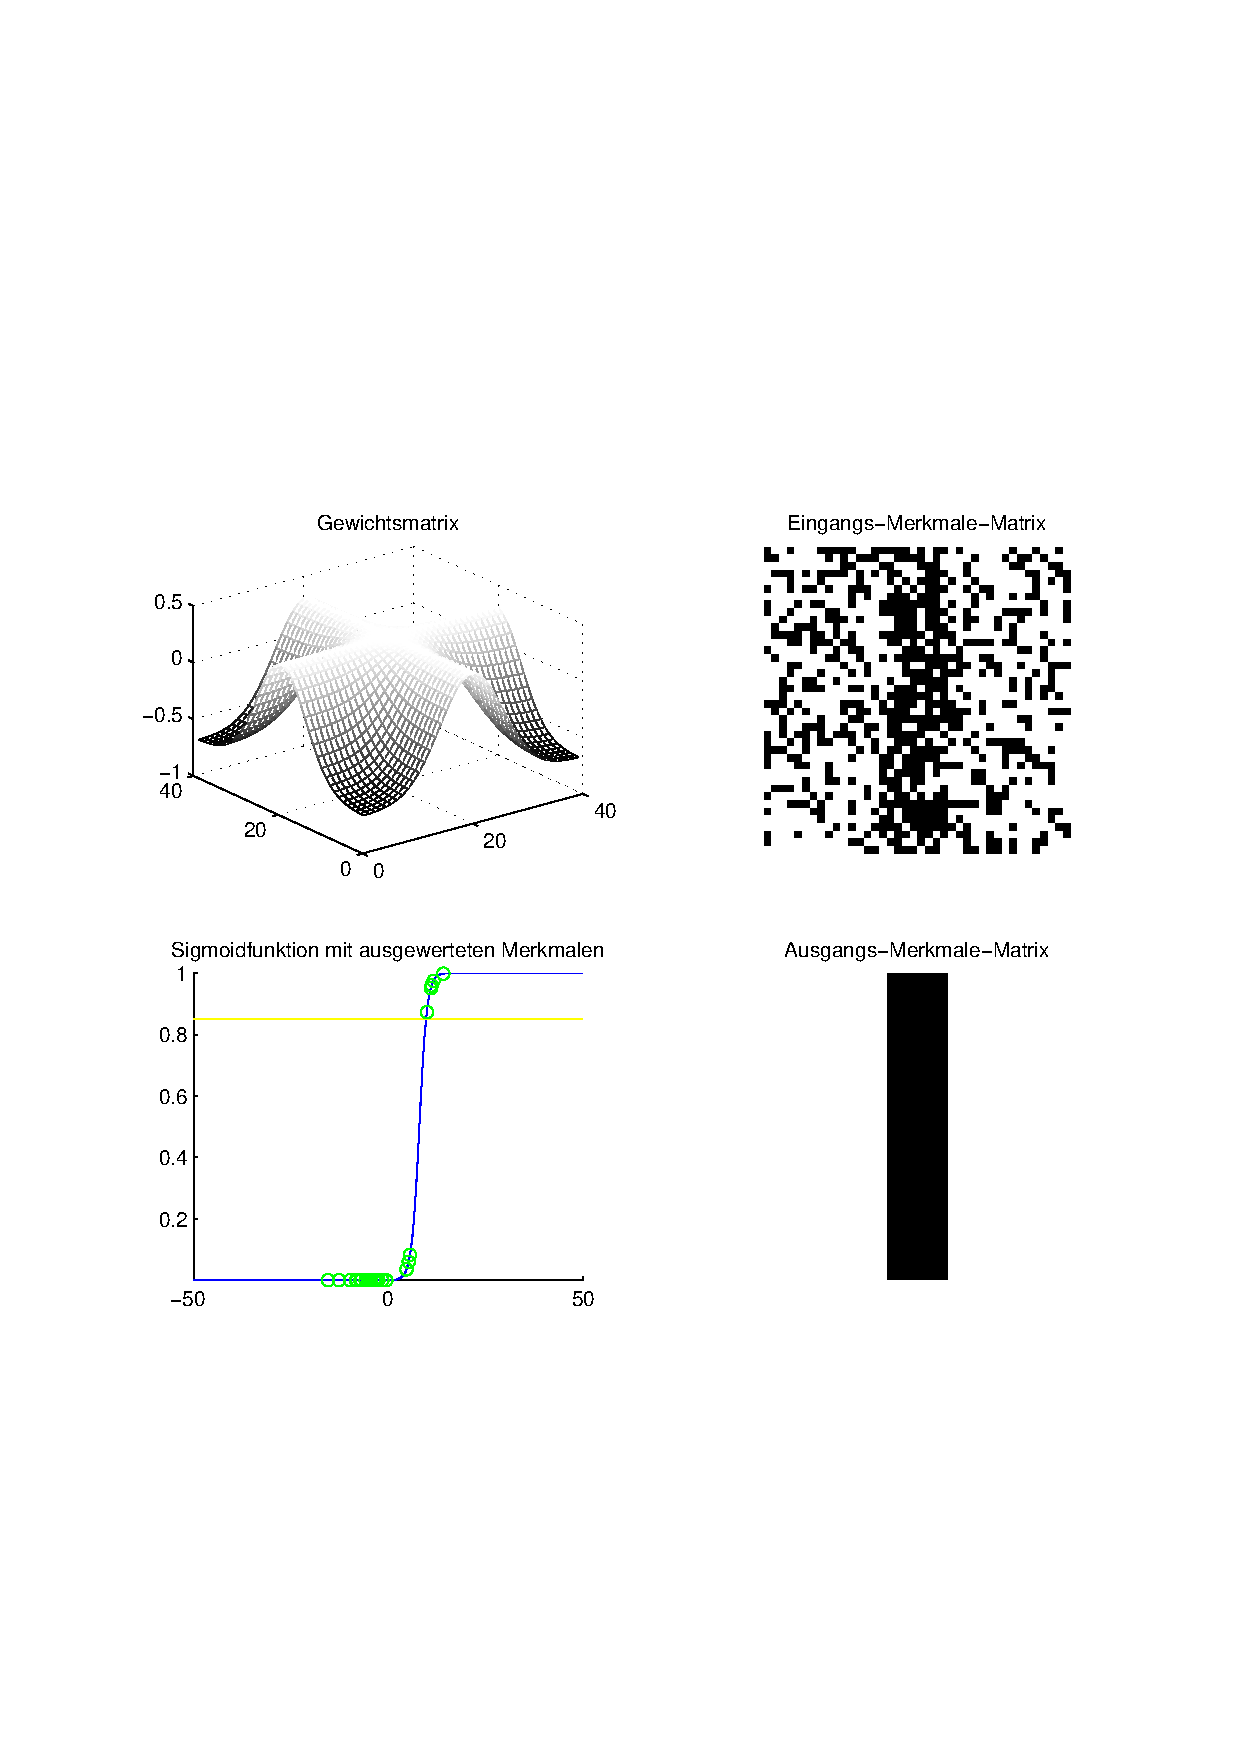
\includegraphics[width=\textwidth]{./Bilder/Auswertung/Endergebnis/TypeAddMul_Rauschen60_V_Line_Layer1}
		\caption{AddMul, V-Balken, 60\% Rauschen, 1. Neuronen Ebene}
		\label{AddMul_V_60_1}
	\end{minipage}
	\vfill
	\begin{minipage}{0.8 \textwidth}
		\includegraphics[width=\textwidth]{./Bilder/Auswertung/Endergebnis/TypeAddMul_Rauschen60_V_Line_Layer2}
		\caption{AddMul, V-Balken, 60\% Rauschen, 2. Neuronen Ebene}
		\label{AddMul_V_60_2}
	\end{minipage}
\end{figure}

\begin{figure}[hbt]
	\begin{minipage}{0.8 \textwidth}
		\includegraphics[width=\textwidth]{./Bilder/Auswertung/Endergebnis/TypeAddMul_Rauschen80_V_Line_Layer1}
		\caption{AddMul, V-Balken, 80\% Rauschen, 1. Neuronen Ebene}
		\label{AddMul_V_80_1}
	\end{minipage}
	\vfill
	\begin{minipage}{0.8 \textwidth}
		\includegraphics[width=\textwidth]{./Bilder/Auswertung/Endergebnis/TypeAddMul_Rauschen80_V_Line_Layer2}
		\caption{AddMul, V-Balken, 80\% Rauschen, 2. Neuronen Ebene}
		\label{AddMul_V_80_2}
	\end{minipage}
\end{figure}
\clearpage

\subsubsection{Kreuz}
\begin{figure}[hbt]
	\begin{minipage}{0.8 \textwidth}
		\includegraphics[width=\textwidth]{./Bilder/Auswertung/Endergebnis/TypeAddMul_Rauschen40_Cross_Layer1}
		\caption{AddMul, Kreuz, 40\% Rauschen, 1. Neuronen Ebene}
		\label{AddMul_Kreuz_40_1}
	\end{minipage}
	\vfill
	\begin{minipage}{0.8 \textwidth}
		\includegraphics[width=\textwidth]{./Bilder/Auswertung/Endergebnis/TypeAddMul_Rauschen40_Cross_Layer2}
		\caption{AddMul, Kreuz, 40\% Rauschen, 2. Neuronen Ebene}
		\label{AddMul_Kreuz_40_2}
	\end{minipage}
\end{figure}

\begin{figure}[hbt]
	\begin{minipage}{0.8 \textwidth}
		\includegraphics[width=\textwidth]{./Bilder/Auswertung/Endergebnis/TypeAddMul_Rauschen60_Cross_Layer1}
		\caption{AddMul, Kreuz, 60\% Rauschen, 1. Neuronen Ebene}
		\label{AddMul_Kreuz_60_1}
	\end{minipage}
	\vfill
	\begin{minipage}{0.8 \textwidth}
		\includegraphics[width=\textwidth]{./Bilder/Auswertung/Endergebnis/TypeAddMul_Rauschen60_Cross_Layer2}
		\caption{AddMul, Kreuz, 60\% Rauschen, 2. Neuronen Ebene}
		\label{AddMul_Kreuz_60_2}
	\end{minipage}
\end{figure}

\begin{figure}[hbt]
	\begin{minipage}{0.8 \textwidth}
		\includegraphics[width=\textwidth]{./Bilder/Auswertung/Endergebnis/TypeAddMul_Rauschen80_Cross_Layer1}
		\caption{AddMul, Kreuz, 80\% Rauschen, 1. Neuronen Ebene}
		\label{AddMul_Kreuz_80_1}
	\end{minipage}
	\vfill
	\begin{minipage}{0.8 \textwidth}
		\includegraphics[width=\textwidth]{./Bilder/Auswertung/Endergebnis/TypeAddMul_Rauschen80_Cross_Layer2}
		\caption{AddMul, Kreuz, 80\% Rauschen, 2. Neuronen Ebene}
		\label{AddMul_Kreuz_80_2}
	\end{minipage}
\end{figure}
\clearpage

\subsection{Special Gewichtsmatrix}
\subsubsection{H-Balken}
\begin{figure}[hbt]
	\begin{minipage}{0.8 \textwidth}
		\includegraphics[width=\textwidth]{./Bilder/Auswertung/Endergebnis/TypeSpecial_Rauschen40_H_Line_Layer1}
		\caption{Special, H-Balken, 40\% Rauschen, 1. Neuronen Ebene}
		\label{Special_H_40_1}
	\end{minipage}
	\vfill
	\begin{minipage}{0.8 \textwidth}
		\includegraphics[width=\textwidth]{./Bilder/Auswertung/Endergebnis/TypeSpecial_Rauschen40_H_Line_Layer2}
		\caption{Special, H-Balken, 40\% Rauschen, 2. Neuronen Ebene}
		\label{Special_H_40_2}
	\end{minipage}
\end{figure}

\begin{figure}[hbt]
	\begin{minipage}{0.8 \textwidth}
		\includegraphics[width=\textwidth]{./Bilder/Auswertung/Endergebnis/TypeSpecial_Rauschen60_H_Line_Layer1}
		\caption{Special, H-Balken, 60\% Rauschen, 1. Neuronen Ebene}
		\label{Special_H_60_1}
	\end{minipage}
	\vfill
	\begin{minipage}{0.8 \textwidth}
		\includegraphics[width=\textwidth]{./Bilder/Auswertung/Endergebnis/TypeSpecial_Rauschen60_H_Line_Layer2}
		\caption{Special, H-Balken, 60\% Rauschen, 2. Neuronen Ebene}
		\label{Special_H_60_2}
	\end{minipage}
\end{figure}

\begin{figure}[hbt]
	\begin{minipage}{0.8 \textwidth}
		\includegraphics[width=\textwidth]{./Bilder/Auswertung/Endergebnis/TypeSpecial_Rauschen80_H_Line_Layer1}
		\caption{Special, H-Balken, 80\% Rauschen, 1. Neuronen Ebene}
		\label{Special_H_80_1}
	\end{minipage}
	\vfill
	\begin{minipage}{0.8 \textwidth}
		\includegraphics[width=\textwidth]{./Bilder/Auswertung/Endergebnis/TypeSpecial_Rauschen80_H_Line_Layer2}
		\caption{Special, H-Balken, 80\% Rauschen, 2. Neuronen Ebene}
		\label{Special_H_80_2}
	\end{minipage}
\end{figure}
\clearpage

\subsubsection{V-Balken}
\begin{figure}[hbt]
	\begin{minipage}{0.8 \textwidth}
		\includegraphics[width=\textwidth]{./Bilder/Auswertung/Endergebnis/TypeSpecial_Rauschen40_V_Line_Layer1}
		\caption{Special, V-Balken, 40\% Rauschen, 1. Neuronen Ebene}
		\label{Special_V_40_1}
	\end{minipage}
	\vfill
	\begin{minipage}{0.8 \textwidth}
		\includegraphics[width=\textwidth]{./Bilder/Auswertung/Endergebnis/TypeSpecial_Rauschen40_v_Line_Layer2}
		\caption{Special, V-Balken, 40\% Rauschen, 2. Neuronen Ebene}
		\label{Special_V_40_2}
	\end{minipage}
\end{figure}

\begin{figure}[hbt]
	\begin{minipage}{0.8 \textwidth}
		\includegraphics[width=\textwidth]{./Bilder/Auswertung/Endergebnis/TypeSpecial_Rauschen60_V_Line_Layer1}
		\caption{Special, V-Balken, 60\% Rauschen, 1. Neuronen Ebene}
		\label{Special_V_60_1}
	\end{minipage}
	\vfill
	\begin{minipage}{0.8 \textwidth}
		\includegraphics[width=\textwidth]{./Bilder/Auswertung/Endergebnis/TypeSpecial_Rauschen60_V_Line_Layer2}
		\caption{Special, V-Balken, 60\% Rauschen, 2. Neuronen Ebene}
		\label{Special_V_60_2}
	\end{minipage}
\end{figure}

\begin{figure}[hbt]
	\begin{minipage}{0.8 \textwidth}
		\includegraphics[width=\textwidth]{./Bilder/Auswertung/Endergebnis/TypeSpecial_Rauschen80_V_Line_Layer1}
		\caption{Special, V-Balken, 80\% Rauschen, 1. Neuronen Ebene}
		\label{Special_V_80_1}
	\end{minipage}
	\vfill
	\begin{minipage}{0.8 \textwidth}
		\includegraphics[width=\textwidth]{./Bilder/Auswertung/Endergebnis/TypeSpecial_Rauschen80_V_Line_Layer2}
		\caption{Special, V-Balken, 80\% Rauschen, 2. Neuronen Ebene}
		\label{Special_V_80_2}
	\end{minipage}
\end{figure}
\clearpage

\subsubsection{Kreuz}
\begin{figure}[hbt]
	\begin{minipage}{0.8 \textwidth}
		\includegraphics[width=\textwidth]{./Bilder/Auswertung/Endergebnis/TypeSpecial_Rauschen40_Cross_Layer1}
		\caption{Special, Kreuz, 40\% Rauschen, 1. Neuronen Ebene}
		\label{Special_Kreuz_40_1}
	\end{minipage}
	\vfill
	\begin{minipage}{0.8 \textwidth}
		\includegraphics[width=\textwidth]{./Bilder/Auswertung/Endergebnis/TypeSpecial_Rauschen40_Cross_Layer2}
		\caption{Special, Kreuz, 40\% Rauschen, 2. Neuronen Ebene}
		\label{Special_Kreuz_40_2}
	\end{minipage}
\end{figure}

\begin{figure}[hbt]
	\begin{minipage}{0.8 \textwidth}
		\includegraphics[width=\textwidth]{./Bilder/Auswertung/Endergebnis/TypeSpecial_Rauschen60_Cross_Layer1}
		\caption{Special, Kreuz, 60\% Rauschen, 1. Neuronen Ebene}
		\label{Special_Kreuz_60_1}
	\end{minipage}
	\vfill
	\begin{minipage}{0.8 \textwidth}
		\includegraphics[width=\textwidth]{./Bilder/Auswertung/Endergebnis/TypeSpecial_Rauschen60_Cross_Layer2}
		\caption{Special, Kreuz, 60\% Rauschen, 2. Neuronen Ebene}
		\label{Special_Kreuz_60_2}
	\end{minipage}
\end{figure}

\begin{figure}[hbt]
	\begin{minipage}{0.8 \textwidth}
		\includegraphics[width=\textwidth]{./Bilder/Auswertung/Endergebnis/TypeSpecial_Rauschen80_Cross_Layer1}
		\caption{Special, Kreuz, 80\% Rauschen, 1. Neuronen Ebene}
		\label{Special_Kreuz_80_1}
	\end{minipage}
	\vfill
	\begin{minipage}{0.8 \textwidth}
		\includegraphics[width=\textwidth]{./Bilder/Auswertung/Endergebnis/TypeSpecial_Rauschen80_Cross_Layer2}
		\caption{Special, Kreuz, 80\% Rauschen, 2. Neuronen Ebene}
		\label{Special_Kreuz_80_2}
	\end{minipage}
\end{figure}
\clearpage


\newpage
\section{Fazit}

In diesem Projekt haben wir ein neuronales Netz zur Detektion von horizontalen und vertikalen Balken entwickelt. Das neuronale Netz besteht dabei aus zwei Neuronen Schichten. Die Anzahl der benötigten Neuronen hängt dabei von der Anzahl der Merkmale ab. Die Anzahl der Neuronen wächst Linear mit der Anzahl der Merkmalen. Die erste Neuronen Ebene fasst dabei alle Pixel zu den jeweiligen Merkmalen zusammen. Jedes Pixel wird dabei über die Gewichts-Matrix bewertet. In der zweiten Neuronen Ebene findet eine Verfeinerung des Ergebnisses statt. Erst die zweite Neuronen Ebene wertet die Informationen aus den Merkmalen aus.

Entwickelt haben wir verschiedene Möglichkeiten von Gewichts-Matrizen. Untersucht haben wir am Ende die zwei erfolgversprechendsten Gewichts-Matrizen 'AddMul' und 'Special'. 'AddMul' hatte dabei die maximale Möglichkeit Parameter einzustellen. Dies ist bei der Special-Gewichtsmatrix nicht möglich. Vergleicht man beide Typen von Gewichts-Matrizen fällt kaum ein Unterschied im Ergebnis auf. Aus diesem Grund ist für uns die AddMul-Gewichts-Matrix besser geeignet, weil sie einfacher aufgebaut und besser einstellbar ist. Bei der Special-Gewichts-Matrix konnte sich ein Vorteil der erhöhten Randbereiche nicht bestätigen. Durch die Erhöhung haben sich lediglich die Schwellen der Detektion verändert.

Um die richtige Konfiguration der verschiedenen Parameter zu finden, haben wir länger gebraucht als erwartet. Es hat sich teilweise als sehr schwierig erwiesen vernünftige Werte zu finden. Die Ergebnisse hängen sehr stark davon ab, wie viel Rauschen man in den Bildern hat. Erste Einstellungen des neuronalen Netzes haben in komplett verrauschten Bildern ein Kreuz detektiert. Durch sukzessive Anpassung der Schwellen haben wir diesen Problem in den Griff bekommen. 

\begin{figure}[hbt]
	\centering
	\includegraphics[width=0.6\linewidth]{./Bilder/Auswertung/MerkmalGruppen}
	\caption{Merkmale-Gruppen}
	\label{mGrup}
\end{figure}

Ein weiteres Problem war es, die Merkmale der ersten Neuronen Ebene in zwei Gruppen zu unterteilen und damit separierbar zu machen. Jede Gruppe soll dabei möglichst zusammenhängend sein. Für das bessere Verständnis siehe Abbildung \ref{mGrup}. In diesem Fall muss die Flanke der Sigmoid-Funktion zwischen den beiden Gruppen liegen. Die Verschiebung der Sigmoid-Funktion wird über den jeweiligen Bias-Parameter erreicht. Mit dem Threshold-Parameter wird die Schwelle festgelegt, ab wann ein aktives Merkmal detektiert werden soll. Werden die Parameter 'pixelCnt', 'featureCnt', 'lowerBound', 'upperBound' oder 'slope' geändert, dann müssen auch die Parameter 'bias', 'threshold' und 'domainOfDefinition' neu eingestellt werden.

Im Gegensatz zur ersten Ebene sind die richtigen Einstellungen für die zweite Ebene deutlich leichter zu finden, weil mal statt einer Sigmoid-Funktion drei Sigmoid-Funktionen zum Einstellen hat. Zur Erinnerung die zweite Neuronen Ebene erhält von der ersten Neuronen Ebene nicht die Werte der Sigmoid-Funktion, sondern die addierten Pixel-Gewichte ohne weitere Verarbeitung. Bei der zweiten Ebene können die Einstellungen für die Detektion des 'H-Balken', 'V-Balken' und des 'Fehlers' unabhängig voneinander eingestellt werden.

Mit dieser Arbeit haben wir einen Meilenstein gelegt, um ein Neuronales Netz in Hardware zu implementieren. Wir haben Erfahrungen gesammelt, wie ein selbst lernendes neuronales Netz die Gewichte findet und wie es aufgebaut sein muss, um vernünftige Ergebnisse zu liefern. Im Weiteren werden wir uns damit befassen unsere Ergebnisse in Hardware zu implementieren.



%------------------------------------------------------------
% Anhang
%------------------------------------------------------------
\newpage
\bibliographystyle{plain}
\bibliography{bibliography}
%\clearpage
%\section{Anhang}
\end{document}